\section{Identification and Estimation of Life-Cycle Treatment Effects} \label{appendix:methodology}

This appendix presents our approach to identify and estimate life-cycle treatment effects. Differences in the approach for each outcome are based on different scenarios of data availability. We proceed as follows. Appendix~\ref{app:method_fullobs} focuses on outcomes that are essentially fully observed over the course of the experiment with little attrition. Appendix~\ref{app:method_partialobs} focuses on outcomes that are partially observed over the course of the experiment with a substantial rate of attrition. Appendix~\ref{app:method_noobs}  focuses on outcomes that we do not observe, and thus need to forecast out of sample. Appendices~\ref{app:method_irr} and ~\ref{app:method_cbratio} provide some technical details on the computations of the internal rate of return and the benefit/cost ratios, respectively. Appendix~\ref{appendix:gmm} frames our data combination problem in the Generalized Method of Moments framework. Finally, Appendix~\ref{appendix:bootstrap} provides the precise steps for constructing our statistical inference.

\subsection{Complete Data}\label{app:method_fullobs}

We classify a variable as having essentially complete data when we observe the data for at least 90\% of the individuals in the sample \textbf{[JJH: Which is it 85\% as in this page or 90\% as on next page?] [JLG: 90\%. That was definitely a mistake.]} Table~\ref{table:nonipw} lists the variables that are completely observed. For these outcomes, we estimate the standard errors of our estimates by resampling the ABC/CARE data with replacement. We estimate non-parametric $p$-values based on the bootstrap distribution.

\begin{table}[H]
\begin{threeparttable}
\caption{Variables Estimated without IPW Adjustment}
\label{table:nonipw}
\centering
% CONTENT CREATED ON SPREADSHEET, TREAT AS A .CSV (TAB DELIMITED)
% CAN BE COPIED INTO A SPREADSHEET PROGRAM (EXCEL, LIBRECALC) FOR EDITING
\begin{tabular}{l l}
\toprule
Variable	&	Age	\\
\midrule			
IQ Standard Score	&	2, 3, 4, 5, 6, 7, 8, 12, 15, 21	\\
PIAT Math Standard Score	&	7	\\
Home Total Score	&	0.5, 1.5, 2.5, 3.5, 4.5, 8	\\
Mother Works	&	2, 3, 4, 5	\\
Biological Mother's Education Level	&	2, 3, 4, 5, 9	\\
Father is Home	&	2, 3, 4, 5	\\
Ever Adopted	&		NA \\
Graduated High School	&	NA	\\
Attended Vocation/Tech/Community College	&	NA	\\
Earned Degree from 4-year College	&	NA	\\
Years of Education	&	30	\\
Works a Job	&	30	\\
Total Felony Arrests	&	Mid-30s	\\
Total Misdemeanor Arrests	&	Mid-30s	\\
Total Years Incarcerated	&	30	\\
Self-reported Health	&	30	\\
Number of Cigarettes Smoked Per Day Last Month	&	30	\\
Number of Days Drank Alcohol Last Month	&	30	\\
Number of Days Binge Drank Alcohol Last Month	&	30	\\
Program Costs	&	0--26	\\
Control Contamination Costs	&	0--26	\\
Education Costs	&	0--26	\\
Medical Expenditure &	8--30	\\
Justice System Costs	&	0--50	\\
Prison Costs	&	0--50	\\
Victimization Costs	&	0--50	\\
\bottomrule			
\end{tabular}
\begin{tablenotes}
\footnotesize
\item Note: The table above lists the variables which we observe completely for the full sample.
\end{tablenotes}
\end{threeparttable}
\end{table}

\subsection{Partially Complete Data}
\label{app:method_partialobs}

When we do not observe data on an outcome for more than 10\% of the individuals in the sample, we consider the outcome to be partially complete. These outcomes include: parental labor income at ages 1.5, 2.5, 3.5, 8, 12, 15, and 21, for which we observe no more than 112 subjects at any given age; and items in the health survey at age 34, for which we observe no more than 93 subjects. Table~\ref{table:attpooled} lists the variables that we classify as partially complete.

\noindent For partially complete outcomes, we correct for attrition using an inverse probability weighting scheme (IPW) as in  \citet{Horvitz_Thompson_1952_JASA}. For each partially observed outcome, we construct an IPW scheme. The weights are based on a set of pre-treatment variables that we observe for the complete sample. We use a set of baseline variables to estimate the propensity of observing the value of a partially complete outcome.  These probabilities are estimated using a logistic regression. The set of baseline variables is chosen among many possible control sets,  as documented in Appendix~\ref{appendix:bvariables}. For each partially observed outcome, we list the variables that we use to produce the IPW scheme in Table~\ref{table:attpooled}. To estimate the standard errors of our estimates, we resample the ABC/CARE data with replacement as in Appendix~\ref{app:method_fullobs}. Each time we resample, we reestimate the IPW weights to account for estimation error. Our standard errors thus account for sampling uncertainty and for estimation error in the computation of the IPW scheme. We estimate non-parametric $p$-values based on the bootstrap distribution.

\noindent \textbf{[JJH: Jorge - The attrition analysis table should go through age 34.] [JLG: An attrition chronology with a corresponding table was added to Appendix~\ref{appendix:background}.]} 

\newgeometry{top=.1in, bottom=.1in, left=.1in, right=.1in}
\begin{sidewaystable}[H]
\begin{threeparttable}
\caption{Variables Used to Create IPW Scheme}
\label{table:attpooled}
\centering
% CONTENT CREATED ON SPREADSHEET, TREAT AS A .CSV (TAB DELIMITED)
% CAN BE COPIED INTO A SPREADSHEET PROGRAM (EXCEL, LIBRECALC) FOR EDITING
\scriptsize
\begin{tabular}{l r r l l l}
\toprule											
Partially Observed Outcomes	&	Age	&	N	&	\multicolumn{3}{c}{Variables Used to Produce IPW}	\\
\midrule	
IQ Score 				& 6.5 	& 126   & High Risk Index (HRI)	& APGAR 1 min.	&  Cohort \\
IQ Score 				& 7 	& 118   & High Risk Index (HRI)	& APGAR 5 min.	&  Cohort \\
IQ Score 				& 8 	& 125   & High Risk Index (HRI)	& APGAR 1 min.	&  Cohort \\
\\										
Achievement Score 		& 5.5	& 105 	& High Risk Index (HRI)	& APGAR 1 min.	&  Cohort \\ 
Achievement Score 		& 6		& 124 	& High Risk Index (HRI)	& APGAR 1 min.	&  Cohort \\ 
Achievement Score 		& 6.5	& 89 	& High Risk Index (HRI)	& APGAR 1 min.	&  Cohort \\ 
Achievement Score 		& 7		& 90 	& High Risk Index (HRI)	& APGAR 1 min.	&  Cohort \\ 
Achievement Score 		& 7.5	& 121 	& High Risk Index (HRI)	& APGAR 1 min.	&  Cohort \\ 
Achievement Score 		& 8		& 123 	& High Risk Index (HRI)	& APGAR 1 min.	&  Cohort \\ 
Achievement Score 		& 8.5	& 122 	& High Risk Index (HRI)	& APGAR 5 min.	&  Cohort \\ 
\\
Parental Labor Income	&	1.5	&	112	& Mother's Age at Baseline	& APGAR 1 min.	&  Cohort \\
 Parental Labor Income	&	2.5	&	112	&	Mother's Age at Baseline	& APGAR 1 min.	&  Cohort \\
 Parental Labor Income	&	3.5	&	110	&	Mother's Age at Baseline	& APGAR 1 min.	&  Cohort \\
 Parental Labor Income	&	8	&	87	&	High Risk Index (HRI)	& APGAR 1 min.	&  Cohort \\
 Parental Labor Income	&	12	&	108	&	High Risk Index (HRI)	& APGAR 1 min.	&  Cohort \\
 Parental Labor Income	&	15	&	92	&	APGAR 5 min. & 	Premature at Birth & Number of Siblings, Baseline \\
 Parental Labor Income	&	21	&	73	&	High Risk Index (HRI)	& APGAR 1 min.	&  Cohort \\
\\
HOME Score				& 8		& 	100 & 	High Risk Index (HRI)	& APGAR 1 min.	&  Cohort \\
\\
Father at Home			& 8		& 	116 & 	High Risk Index (HRI)	& APGAR 1 min.	&  Cohort \\
\\
Subject Public Transfer Income	&	21	&	105	& High Risk Index (HRI) & APGAR 1 min. & Cohort \\
 \\
Total Felony Arrests		& Mid-30s	& 115 &	APGAR 1 min. & APGAR 5 min. & Cohort	\\
Total Misdemeanor Arrests	& Mid-30s	& 115 &	APGAR 1 min. & APGAR 5 min. & Cohort	\\
 \\
 Self-reported Health	&	Mid-30s	&	92	&	APGAR 1 min. & APGAR 5 min. & Premature at Birth	\\
 Self-reported Drug User	&	Mid-30s	&	89	&	APGAR 1 min. & APGAR 5 min. & Premature at Birth	\\
 Systolic Blood Pressure (mm Hg)	&	Mid-30s	&	90	&	APGAR 1 min. & Premature at Birth & Number of Siblings, Baseline	\\
 Diastolic Blood Pressure (mm Hg)	&	Mid-30s	 &	90	&	APGAR 1 min. & Premature at Birth & Number of Siblings, Baseline	\\
 Prehypertension, Sys. B.P. $>$ 120 or Dys. B.P. $>$ 80	&	Mid-30s	&	90	&	APGAR 1 min. & Premature at Birth & Number of Siblings, Baseline	\\
 Hypertension, Sys. B.P. $>$ 140 or Dys. B.P. $>$ 90	&	Mid-30s	&	90	&	APGAR 1 min. & Premature at Birth & Number of Siblings, Baseline	\\
 High-Density Lipoprotein (HDL) Cholesterol (mg/dL)	&	Mid-30s	&	93	&	APGAR 1 min. & Premature at Birth & Number of Siblings, Baseline	\\
 Dyslipidemia (HDL $<$ 40 mg/dL)	&	Mid-30s	&	93	&	APGAR 1 min. & Premature at Birth & Number of Siblings, Baseline	\\
 Hemoglobin Level (\%)	&	Mid-30s	&	92	&	APGAR 1 min. & Premature at Birth & Number of Siblings, Baseline	\\
 Prediabetes, Hemoglobin $>$ 5.7\%	&	Mid-30s	&	92	&	APGAR 1 min. & Premature at Birth & Number of Siblings, Baseline	\\
 Diabetes, Hemoglobin $>$ 6.5\%	&	Mid-30s	&	92	&	APGAR 1 min. & Premature at Birth & Number of Siblings, Baseline	\\
 Vitamin D Deficiency ($<$ 20 ng/mL)	&	Mid-30s	&	93	&	APGAR 1 min. & Premature at Birth & Number of Siblings, Baseline	\\
 Measured BMI	&	Mid-30s	&	88	&	APGAR 1 min. & APGAR 5 min. & Premature at Birth \\
 Obesity (BMI $>$ 30)	&	Mid-30s	&	90	&	APGAR 1 min. & APGAR 5 min. & Premature at Birth \\
 Severe Obesity (BMI $>$ 35)	&	Mid-30s	&	91	&	APGAR 1 min. & APGAR 5 min. & Premature at Birth \\
 Waist-hip Ratio	&	Mid-30s	&	84	& APGAR 1 min. & Premature at Birth & Number of Siblings, Baseline \\
 Abdominal Obesity	&	Mid-30s	&	84	& APGAR 1 min. & Premature at Birth & Number of Siblings, Baseline \\
 Framingham Risk Score	&	Mid-30s	&	88	& APGAR 1 min. & Premature at Birth & Number of Siblings, Baseline \\
 Brief Symptom Survey (BSI) Score & Mid-30s & 92 &	APGAR 1 min. & APGAR 5 min. & Premature at Birth	\\
\bottomrule											
\end{tabular}
\begin{tablenotes}
\footnotesize
\item Note: This table lists the partially observed variables and the variables that we use to construct the IPW scheme to account for attrition when calculating treatment effects. The procedure to select these variables is described in Appendix~\ref{appendix:bvariables}. We construct the IPW scheme using a common model across males and females.
\end{tablenotes}
\end{threeparttable}
\end{sidewaystable}
\restoregeometry
\doublespacing

\noindent Partially observed outcomes can occur at any age $a \leq a^*$.\footnote{After $a^*$, we have incomplete data and do not observe any outcome. We explain the details for constructing predictions in Appendix~\ref{appendix:incomplete}.} We construct the IPW scheme using pre-treatment variables, within the age period  $a \leq a^*$.

\noindent We construct the IPW scheme using the same algorithm, independent of the age $a$ for $a \leq a^*$ in which an outcome is partially complete. For notational simplicity, we derive the IPW scheme without indexing the outcomes by age or treatment status (we estimate IPW using a common logistic regression across treatment regimes to avoid instability in the estimates that could be a problem in our small experimental sample). We restore the notation used throughout the text in the next appendix. \\

\noindent We use a standard inverse probability weighting (IPW) scheme.\footnote{\citet{Horvitz_Thompson_1952_JASA}.} Formally, recall that $R = 1$ if the child is randomized into treatment, and $R = 0$ otherwise.\footnote{We are able to use $R$ (randomization into treatment) and $D$ (participation in treatment) exchangeably as we argue in Section~\ref{section:cbamethodology}.} Similarly, let $A = 1$ denote the case where we observe a generic scalar outcome $Y$ (which is a generic entry in the vector of outcomes that we use in the paper), and $A = 0$ otherwise. As in the main text, $\bm{B}$ represents background (pre-treatment) variables.

\noindent We assume $A$ is independent of $Y$ conditional on $\bm{B}$. More formally, we invoke

\begin{assumption} \label{ass:attr}
	\begin{align*}
		A \independent Y | \bm{B}, R.
	\end{align*}
\end{assumption}

\noindent Let $Y^{r}$ represent outcome $Y$ when $R$ is fixed to take the value $r$. Based on Assumption~\ref{ass:attr}, we use IPW to identify $\mathbb{E}[Y^r]$ as follows:

\begin{align} \label{eq:case2}
\mathbb{E}[Y^r] & = \int \int y f_{ Y^{r}| \bm{B} } (y) f_{\bm{B}} (b) dydb \\ \nonumber
	           & = \int \int y f_{Y| \bm{B}, R=r}(y) f_{\bm{B}} (b) dydb \\ \nonumber
		& = \int \int y f_{Y|\bm{B},R=r, A=1} (y) f_{\bm{B}} (b) dydb
\end{align}

\noindent where each component of the last expression in \eqref{eq:case2} is straightforward to recover from the data. Using Bayes' Theorem, we can write an equivalent expression to make the IPW scheme explicit. That is, we apply Bayes' Theorem to $f_{\bm{B}} (b)$ to obtain

\begin{equation*}
	f_{\bm{B}} (b) = \frac{f_{\bm{B}|R=r,A=1} (b) P(R=r,A=1)}{P(R=r,A=1|\bm{B})}.
\end{equation*}
\noindent Substituting these expressions into \eqref{eq:case2}, we obtain

\begin{align*} \label{eq:case2ipw}
\mathbb{E}[Y^r] & = \int \int y f_{Y,\bm{B}|R=r,A=1}(y,b) \frac{P(R=r,A=1) P(A=1|R=r,\bm{B})}{P(R=r,A=1|\bm{B}) P(A=1|R=r,\bm{B})} dydb \\
	            & = \int \int  y f_{Y,\bm{B}|R=r,A=1}(y,b) \frac{P(R=r,A=1)}{P(R=r|\bm{B}) P(A=1|R=r,\bm{B})} dydb. \\
\end{align*}

\noindent Assumption \ref{ass:attr} generalizes \textbf{[AZ: Without $\bm{X}$, is this still true?]} the matching assumption of \citet{Campbell_Conti_etal_2014_EarlyChildhoodInvestments}. The corresponding sample estimator for $\mathbb{E}[Y^r]$ is

\begin{align*}
\sum_{i \in \mathcal{I}} y_i \beta_{i} \bm{\mathit{1}}(r_i = r) \bm{\mathit{1}}(a_i = 1)
\end{align*}
\noindent where $\mathcal{I}$ indexes the individuals in the sample. As in the paper that lowercase variables $r$, $y$, and $b$ denote realizations of the random variables $R$, $Y$, and $\bm{B}$, respectively.

\begin{align*}
	\beta_{i} = \frac{1}{\pi_r(b_i) \alpha(r_i,b_i)} \frac{1}{\sum_{k \in \mathcal{I}}{\frac{ \bm{\mathit{1}}(r_i = r)  \bm{\mathit{1}}(a_i = 1)}{\pi_r(b_k)\alpha(r_k,b_k)}}},
\end{align*}
\noindent with $\pi_r(b) := P(R=r|\bm{B}=b)$ and $\alpha(r,b) := P(A=1|R=r,\bm{B}=b)$. The weight $\pi_r$ corrects for selection into treatment based on pre-treatment variables $\bm{B}$. The weight $\alpha$ corrects for item non-response based on $R, \bm{B}$.

\noindent In Tables~\ref{table:bcsens} and \ref{table:irrsens}, we present estimates of the internal rate of return and the benefit cost-ratio with and without adjusting for IPW. There is little sensitivity of our estimates to these adjustments.

\subsection{Incomplete Data: Forecasting and Monetizing Life-Cycle and Costs and Benefits} \label{appendix:incomplete}
\label{app:method_noobs}

\noindent We do not observe certain post-$a^*$ life-cycle profiles for outcomes that are important for estimating the lifetime benefits of ABC/CARE. Examples include parental labor income, subject labor income, public-transfer income, and health-related outcome variables. In Section~\ref{section:cbamethodology} to identify and estimate these profiles and forecast post-$a^\ast$ outcomes.This appendix documents how we implement this strategy and provides complementary evidence supporting it, cited throughout the main text. We devote separate appendices to the discussion of crime and health forecasts in Appendix~\ref{appendix:crime} and Appendix~\ref{appendix:health}, respectively.\footnote{In this section, attrition or partial observations is not an issue: the predictors that we use to construct out-of-sample forecasts are classified as complete data (see Appendices~\ref{app:method_fullobs} and \ref{app:method_partialobs}).} 

\subsubsection{Conditions for Valid Out-of-Sample Forecasts}

Forecasting does not require that we take a position on the exogeneity of $\bm{X}^d_{k,a}$ for $k \in \{e,n\}$ and $a \in \{ a, \ldots \bar{A} \}$ with respect to labor income. Estimated structural models with biased parameters can still give reliable forecasts if relationships between observed and unobserved variables are the same within sample and in the forecast sample. Conditions~\ref{cond:cond1} to~\ref{cond:cond3} spell out these requirements, dropping age indexing for simplicity. In the paper, we rely on Assumptions~\ref{ass:summary} and~\ref{ass:exog} because it facilitates the use of economic theory to interpret treatment effects, to forecast outcomes in samples where inputs are manipulated differently than in the experimental sample, and to test the validity of the construction of our synthetic cohort. 

\noindent A strong sufficient condition for identifying the distribution of life-cycle profiles of individuals in the experimental sample using individuals in the auxiliary samples is Condition~\ref{cond:cond1}:

\onehalfspacing
\begin{condition} \textbf{Equality of Distributions Across the Experimental and Auxiliary Samples \label{cond:cond1}}
\begin{equation}
F_{\bm{Y}_e^d, \bm{X}_e^d | \bm{B}_e = \bm{b}} \left( \cdot, \cdot \right) = F_{\bm{Y}_n^d, \bm{X}_n^d | \bm{B}_n = \bm{b}} \left( \cdot, \cdot \right), \quad d \in \{0,1\}
\end{equation}
\noindent for $\bm{Y}_e^d, \bm{X}^d_e | \bm{B}_e = \bm{b}$ and $\bm{Y}_n^d, \bm{X}^d_n | \bm{B}_n = \bm{b}$ contained in the support of the experimental sample $supp\left(\bm{Y}^d_{e}, \bm{X}^d_{e}, \bm{B}_{e} \right)$.
\end{condition}
\doublespacing

\noindent  Since we are only interested in means for benefit/cost analysis, we can get by with a weaker requirement for conditional means:

\onehalfspacing
\begin{condition} \textbf{Equality in Conditional Expectations Across the Experimental and Auxiliary Samples \label{cond:cond2}}
\begin{equation}
\mathbb{E} \left[ \bm{Y}_e^d |  \bm{X}_e^d = \bm{x}, \bm{B}_e = \bm{b} \right] = \mathbb{E} \left[ \bm{Y}_n^d |  \bm{X}_n^d = \bm{x}, \bm{B}_n = \bm{b} \right], \quad d \in \{0,1\}
\end{equation}
for $d \in \{0, 1 \}$ over $supp\left(\bm{Y}^d_{e,a}, \bm{X}^d_{e,a}, \bm{B}_e\right)$.
\end{condition}
\doublespacing

\noindent Since we are primarily interested in treatment effects, we can get by with an even weaker condition:

\onehalfspacing
\begin{condition} \textbf{Equality in Mean Treatment Effects Across the Experimental and Auxiliary Samples \label{cond:cond3}}
\begin{equation}
\mathbb{E} \left[ \bm{Y}_e^1 - \bm{Y}_e^0 | \bm{B}_e = \bm{b} \right] = \mathbb{E} \left[ \bm{Y}_n^1 - \bm{Y}_n^0 | \bm{B}_n = \bm{b} \right]
\end{equation}
over $supp\left(\bm{Y}^d_{e,a}, \bm{B}_e\right)$.\footnotemark
\end{condition}
\footnotetext{We test the difference between the observed and forecasted treatment effect, because as we describe above, an equal difference (as opposed to equal levels) is sufficient. Even though the point estimate of the difference is 2,037.08 ($-$2,256.09) for males (females, we find that this difference is not statistically different than 0 for both genders).}
\doublespacing
We could simply invoke these conditions and be done. Our approach is to examine and test (when possible) assumptions that justify the treatment effects, and that is why we develop the theory in Section~\ref{section:cbamethodology} instead of simply invoking these assumptions.

\subsubsection{Auxiliary Datasets} \label{app:datasets}

\noindent We rely on the following datasets to estimate life-cycle transfer and labor income profiles.\footnote{At age 21, public-transfer income includes Aid to Families with Dependent Children (AFDC) subsidies, food stamps, survivor benefits, disability benefits, social security, rent subsidies, and fuel subsidies. At age 30, public-transfer income includes food stamps, welfare, housing assistance, workman's compensation, disability, social security, supplemental security income, unemployment benefits, worker's compensation insurance, fuel subsidies, educational and aid grants, and other forms of welfare. For all other ages, we produce a forecast. We explain and justify the variables we use to forecast below.} We use some of these same and other complementary sources to forecast the rest of the outcomes, as we explain below.

\noindent\textbf{The National Longitudinal Survey of Youth (NLSY79)} is a longitudinal survey beginning in 1979 that follows individuals born between 1957 and 1964. The initial interview included 12,686 respondents aged 14 to 22. The survey was designed to include 6,111 individuals representing the non-institutionalized civilian population, a supplemental sample of 5,295 civilian Hispanics, Latinos, Blacks, non-Blacks/non-Hispanics, and economically disadvantaged youth, and a sample of 1,280 who served in the military as of September 30, 1978. When appropriately weighted, the NLSY79 is nationally representative of the youth living in the U.S. on January 1, 1979. We include individuals from all three subsamples in our analysis.

\noindent The NLSY79 collected data on labor market participation, education, family background, family life, health, assets and income, government program participation, and measures of cognitive skills.

\noindent We restrict the NLSY79 sample to Blacks with labor incomes less than \$300,000 (2014 USD) at any given year to avoid estimating our forecasts with outliers in the auxiliary sample.\footnote{For details on how we match the individuals in the experimental sample to the individuals in the non-experimental sample, see Appendix~\ref{appendix:match}.} With the mean labor income (2014 USD) in the ABC/CARE sample being \$32,782 at age 30, and the maximum reported being \$189,938, the cut-off we impose on the auxiliary data is high enough so that the labor income support at age 30 in ABC/CARE is contained in the support of labor income at age 30 in the NLSY79.\footnote{For labor income at age 21, we use the CNLSY.}\\

\noindent We do not impose a restriction on the birth year for the NLSY79 as all respondents are between 47 and 55 years of age at the time of the last interview (conducted in 2012). This age range is within the 31--67 range for which we extrapolate the income of the ABC/CARE subjects.

\noindent Given the biennial nature of the NLSY79, we only observe each subject at either odd or even ages. Not only does this reduce the size of the sample on which we fit our forecasting model at each age, but it can introduce biases associated with the odd-aged and even-aged cohorts. To address this issue, we linearly interpolate the variables in the NLSY79 data that are used in our forecasting model. This allows us to estimate our model on all subjects of the NLSY79 satisfying the eligibility conditions $\bm{B}_n \in\mathcal{B}_0$ at every age.

\noindent\textbf{The Children of the National Longitudinal Survey of Youth (CNLSY)} is a survey of the children of the mothers from the NLSY79, beginning in 1986. At the time of the initial interview, the ages of the children surveyed ranged from 0 to 23. As of 2010, the CNLSY sample includes 11,504 children born to NLSY79 mothers. With appropriate weights, the CNLSY may be considered nationally representative of children born to women who were age 14 to 22 in 1979. Interviews were conducted annually between 1986 and 1994, and biennially thereafter.

\noindent Similar to the NLSY79, the CNLSY collected data on cognitive ability, motor and social development, home environment, health information, education, attitudes, employment, income, family decisions, and more.

\noindent As we did with the NLSY79 and for the same reasons, we restrict the CNLSY sample to Black individuals with labor income less than \$300,000 (2014 USD) at any given year. In addition to this, we limit the sample to subjects born between 1978 and 1983. Because the CNLSY data extends to 2012, we use the most recent data from the CNLSY in which individuals are aged 29 to 34. Finally, given the biennial nature of the survey, we perform a linear interpolation on the variables that enter into our forecasting model. This allows us to use as much of the CNLSY data as possible at every age when interpolating subject income.

\noindent\textbf{The Panel Survey of Income Dynamics (PSID)} is a longitudinal household survey containing between 5,000 and 8,500 families in each wave. It began as a yearly survey in 1968 and has been fielded biennially since 1996. When appropriately weighted, the PSID is designed to be representative of U.S. households. The PSID provides extensive information concerning demographics, economic outcomes, health outcomes, marriage and fertility, and more.

\noindent We restrict the PSID to Blacks born between 1945 and 1981. Because the data extend to 2013, we use the most recent subsample of individuals aged 30 to 67. We also exclude all individuals with labor income exceeding \$300,000 (2014 USD) in any given year for the same reasons. Finally, given the biennial nature of the survey, we perform a linear interpolation on the variables that enter into our forecasting model. This allows us to use as much of the PSID data as possible at every age to interpolate subject income.

\noindent Before summarizing, note that in general: (i) \textbf{we use the CNLSY to predict from ages 21 to 29}; and (ii) we use the NLSY79 and PSID to forecast from ages 29 to 79. Whenever using the NLSY79 and PSID together, we combine them and use them as a joint sample. Put differently, we use the three data sets to obtain information across our time span of interest \textit{without placing specific weights in any particular samples}. This allows us to satisfy support conditions (see Appendix~\ref{app:containsupport}) over the forecasted variables and the predictors that we use. An alternative to this is to to weight each of the observations in these samples according to the inverse of their variance in a set of observed characteristics. We do not do this, and instead use the unweighted observations to then construct synthetic treatment and controls groups as we explain in Appendix~\ref{appendix:match}.

\noindent \textbf{Summary: Initial Restrictions Placed on the Auxiliary Samples}\\
When constructing the samples used to forecast transfer and labor income, we place the following restrictions on the admissible samples \textit{for all ages}. Additional restrictions are placed when forecasting the other outcomes, as we explain below.
\begin{enumerate}
\item \textbf{NLSY79:} Black, labor income less than \$300,000 (2014 USD) at any given year; subjects born between 1957 and 1965.
\item \textbf{PSID:} Black;  labor income less than \$300,000 (2014 USD) at any given year; birth year between 1945 and 1981.
\item \textbf{CNLSY:} Black, labor income less than \$300,000 (2014 USD) at any given year; subjects born between 1978 and 1983.
\end{enumerate}

\noindent \textbf{Summary: Auxiliary Samples Used to Forecast by Age}\\
We use the following samples to forecast labor and transfer income. Different samples are used to forecast the rest of the outcomes, as we explain below.
\begin{enumerate}
\item \textbf{Labor Income:}
\begin{enumerate}
\item \textbf{Ages 21 to 29:} CNLSY.
\item \textbf{Ages 29 to 67 (assumed age of retirement):} NLSY79 and PSID.
\end{enumerate}
\item \textbf{Transfer Income:}
\begin{enumerate}
\item \textbf{Ages 21 to 29:} CNLSY.
\item \textbf{Ages 29 to 79 (we assume no transfers other than health-related after age 79):} NLSY79 and PSID.
\end{enumerate}
\end{enumerate}

\subsubsection{Constructing Synthetic Cohorts}\label{appendix:match}

\noindent Once the initial restrictions are placed on the auxiliary samples, we weight the observations in the non-experimental sample using the following algorithm: 

\onehalfspacing
\begin{algorithm} \label{alg:match}
For individual $i$ in experimental sample ($k=e$), an individual $l(i)$ in the auxiliary sample ($k=n$) is a potential counterpart if

\begin{equation}\label{eq:ingrownnail}
\sqrt{(\bm{B}_{i,e} - \bm{B}_{i,l(i),n})^\prime (\bm{\Sigma}_e)^{-1} (\bm{B}_{i,e} - \bm{B}_{i,l(i),n})} \leq \epsilon
\end{equation}

\noindent where $\bm{B}_{i,l(i),n}$ represents the observed characteristics of the matched potential counterpart in the non-experimental sample and $\bm{\Sigma}_e$ is the covariance matrix in the experimental sample. As explained in the paper, this procedure is done based on baseline variables that do not change over the life cycle and are not affected by treatment. Thus, this procedure is \textit{not} done age by age. One synthetic cohort is constructed in each of the non-experimental samples by weighting the potential counterparts according to the inverse value of the left-hand-side of Equation~\eqref{eq:ingrownnail}.\footnote{In practice, we set $\epsilon = 1$, but we try a range of values between 0.5 and 3 finding little sensitivity. The full set of the results we produce in the paper for multiple values in the interval [0.5,3] is available on request.}
\end{algorithm}
\doublespacing

\noindent We estimate dynamic relationships between outcomes and predictors in the auxiliary samples and use the estimated relationships to generate forecasts in the non-experimental samples. When producing these estimates, we use our synthetic cohort (i.e.,\ our weighted the auxiliary samples).

\noindent \textbf{Summary: Variables Used to Match to Construct Synthetic Cohorts}\\
When constructing synthetic cohorts using each of the following variables, \textit{for all the outcomes}: year of birth, gender, number of siblings at baseline. The criterion for selecting these variables is availability across all auxiliary sources. We construct one synthetic cohort in each auxiliary sample.

\subsubsection{Variables Used to Forecast Out-of-Sample Outcomes} \label{appendix:pred}

\noindent \textbf{Criteria for Candidate Predictor Variables}\\
\noindent To be considered a predictor variable, a variable must satisfy three conditions: (i) it has to be available in the experimental and non-experimental samples; (ii) it has to have predictive power for the predicted outcome. Our criterion for inclusion is that all the coefficients of a regression of the predicted variable on \textit{all} the prediction variables are chosen to be statistically significant at the 1\% level.\footnote{In a few cases, we decide to keep some variables nearly above this threshold because we consider them economically relevant.}; and (iii) it needs to satisfy Assumption~\ref{ass:contain}, which we document below in Appendix~\ref{app:containsupport}.\footnote{A more logical way to proceed would be to use a sub-sample of predictors satisfying this criteria and also being affected by treatment, so that we are able to predict treatment effects. This is impossible due to data limitations. Most of the post-treatment predictors we use, however, display sizable treatment effects. See Appendix~\ref{appendix:results}.}\\

\noindent For a variable to satisfy restrictions (i) and (ii), it needs to be the case not only that the variable is available in the non-experimental sample but also that the survey question for it was introduced far enough back in time for us to observe it in a range that is common to the range in which we observe the variables in the experimental sample. To illustrate this, consider the case of body-mass index in the PSID. Survey questions for this variable were introduced in the late 1990s. The sample for which the question was introduced, however, does not span enough observations for its support to cover the support of the experimental sample. To lessen this problem we pool the auxiliary datasets to maximize the available predictor variables.

\noindent We present evidence on the predictive power of the predictor variables in the synthetic cohorts that we constructed in the PSID, NLSY79, and CNLSY. Tables~\ref{table:predlaborincome} and \ref{table:predtransferincome} show that, in each of the auxiliary samples that we use, the prediction variables $\bm{X}_{n,a}^d, \bm{B}_n$ are strong predictors of labor and transfer income at age 30. We present this evidence at age 30 both for brevity.

\noindent \textbf{Summary: Predictor Variables}\\
\noindent We use the following variables to forecast labor and transfer income. Different variables are used to forecast the rest of the outcomes, as we explain below.
\begin{enumerate}
\item \textbf{Labor Income:}
\begin{enumerate}
\item \textbf{Ages 22 to 30:} male, mother's education at birth, average PIAT Mathematics score from ages 5 to 7, years of education at age 30, one-year lagged labor income.
\item \textbf{Ages 31 to 67 (assumed age of retirement):} male, years of education at age 30, labor income at age 30, one-year lagged labor income.
\end{enumerate}
\item \textbf{Transfer Income}
\begin{enumerate}
\item \textbf{Ages 21 to 30:} male, mother's education at birth, average PIAT Mathematics score from ages 5 to 7, years of education at age 30, transfer income at age 21, one-year lagged transfer income.
\item \textbf{Ages 31 to 67 (we assume no transfers other than health-related after age 79):} male, years of education at age 30, labor income at age 30, one-year lagged transfer income.
\end{enumerate}
\end{enumerate}

\begin{sidewaystable}[H]
\begin{threeparttable}
\caption{Predictors of Labor Income at Age 30, Auxiliary Sources}
\label{table:predlaborincome}
\centering
\footnotesize
\begin{tabular}{lcccccc} \toprule
 & (1) & (2) & (3) & (4) & (5) & (6) \\
Group Matched   & Control & Treatment & Control & Treatment  & Control & Treatment \\ 
Auxiliary Sample & \multicolumn{2}{c}{CNLSY} & \multicolumn{2}{c}{NLSY79}  & \multicolumn{2}{c}{PSID} \\  \midrule 
Male & 3,999.07*** & 3,911.59*** & 2,633.17*** & 2,616.23*** & 7,087.28*** & 7,096.48*** \\
 & (1,264.39) & (1,211.81) & (401.89) & (378.45) & (888.77) & (891.09) \\
Black & -3,366.02*** & -3,175.47*** & -1,236.27*** & -1,236.89*** & -1,900.33*** & -1,926.12*** \\
 & (1,149.44) & (1,128.24) & (330.86) & (307.09) & (489.68) & (493.72) \\
PIAT (5-7) & 83.87 & 79.94 &  &  &  &  \\
 & (60.09) & (57.83) &  &  &  &  \\
Education (30) & 2,274.99*** & 2,224.96*** & 845.98*** & 833.57*** & 1,813.90*** & 1,824.82*** \\
 & (410.42) & (394.57) & (132.05) & (121.78) & (195.01) & (196.46) \\
Labor Income (21) & 0.13** & 0.13** & 0.13** & 0.13** & 0.06* & 0.06* \\
 & (0.06) & (0.06) & (0.07) & (0.06) & (0.03) & (0.03) \\
Lagged Labor Income  & 0.53*** & 0.55*** & 0.87*** & 0.88*** & 0.72*** & 0.72*** \\
 & (0.07) & (0.07) & (0.06) & (0.06) & (0.05) & (0.05) \\
Constant & -25,579.06*** & -25,100.97*** & -8,339.73*** & -8,190.57*** & -16,127.27*** & -16,235.51*** \\
 & (6,453.86) & (6,262.12) & (1,354.43) & (1,249.59) & (1,968.18) & (1,982.72) \\ \\ \midrule
Observations & 1,215 & 1,215 & 7,036 & 8,219 & 5,544 & 5,544 \\
$R^2$  & 0.51 & 0.52 & 0.65 & 0.65 & 0.61 & 0.61 \\ \bottomrule
\end{tabular}

\begin{tablenotes}
\footnotesize
\item Note: All columns display regressions of labor income at age 30 on the different variables listed in the rows. If the space for the coefficient appears empty, it was not included in the regression. All money figures are in 2014 USD. The number in parentheses next to the variable indicates the age of measurement. Education is measured as years of education. Robust standard errors are in parentheses below the estimates. We weigh the individuals in the auxiliary samples to match them on observed individual characteristics using the procedure in Appendix~\ref{appendix:match}. $^{***}$: $p$-value $< .01$. $^{**}$: $p$-value $< .05$. $^{*}$: $p$-value $< .10$.
\end{tablenotes}
\end{threeparttable}
\end{sidewaystable}

\begin{table}[H]
\begin{threeparttable}
\caption{Predictors of Transfer Income at Age 30, Auxiliary Sources}
\label{table:predtransferincome}
\centering
\footnotesize
\begin{tabular}{lcccc} \toprule
 & (1) & (2) & (3) & (4)  \\
Group Matched   & Control & Treatment & Control & Treatment \\ 
Auxiliary Sample & \multicolumn{2}{c}{NLSY79} & \multicolumn{2}{c}{PSID}  \\  \midrule 
Male & -167.28*** & -166.06*** & -515.30*** & -515.46*** \\
 & (36.72) & (35.08) & (155.70) & (155.49) \\
Black & 116.95*** & 123.03*** & 136.30 & 135.77 \\
 & (44.04) & (42.49) & (143.46) & (143.13) \\
Education (30) & -44.70*** & -43.84*** & -103.94** & -103.93** \\
 & (6.38) & (6.15) & (42.35) & (42.23) \\
Transfer Income (21)& 0.11*** & 0.11*** & 0.11*** & 0.11*** \\
 & (0.03) & (0.03) & (0.03) & (0.03) \\
Lagged Transfer Income & 0.63*** & 0.64*** & 0.64*** & 0.64*** \\
 & (0.03) & (0.03) & (0.04) & (0.04) \\
Constant & 871.56*** & 855.82*** & 1,950.42*** & 1,950.78*** \\
 & (101.41) & (97.62) & (600.85) & (599.32) \\ \\ \midrule
Observations & 7,127 & 8,306 & 1,539 & 1,539 \\
$R^2$  & 0.48 & 0.48 & 0.58 & 0.57 \\ \bottomrule
\end{tabular}

\begin{tablenotes}
\footnotesize
\item Note: All columns display regressions of labor income at age 30 on the different variables listed in the rows. If the space for the coefficient appears empty, it was not included in the regression. All money figures are in 2014 USD. The number in parentheses next to the variable indicates the age of measurement. Education is measured as years of education. Robust standard errors are in parentheses below the estimates. We weigh the individuals in the auxiliary samples to match them on observed individual characteristics using the procedure in Appendix~\ref{appendix:match}. $^{***}$: $p$-value $< .01$. $^{**}$: $p$-value $< .05$. $^{*}$: $p$-value $< .10$.
\end{tablenotes}
\end{threeparttable}
\end{table}

\paragraph{Non-Parametric Forecasts} \label{appendix:nonpar}

\noindent An alternative to the forecasting strategy that we use throughout the main text and the preceding appendix, is the following. For each individual ($i$) in the experimental sample ($e$), we can: (i) find a match or a set of matches in the auxiliary sample ($n$) using a modified version of Algorithm~\ref{alg:match} that includes both baseline variables and variables affected by treatment. Dropping age indices, the modified algorithm is: 

\begin{algorithm} \label{alg:match}
For individual $i$ in experimental sample ($k=e$), an individual $l(i)$ in the auxiliary sample ($k=n$) is a potential counterpart if

\begin{equation}\label{eq:ingrownnail}
\sqrt{(\bm{Z}_{i,e}^d - \bm{Z}_{i,l(i),n}^d)^\prime (\bm{\Sigma}_e)^{-1} (\bm{Z}_{i,e}^d - \bm{Z}_{i,l(i),n}^d)} \leq \epsilon
\end{equation}

\noindent where $\bm{Z}_{i,k}^d:= \left[ \bm{X}_{i,k}^d , \bm{B}_{i,k} \right]$ and $\bm{Z}_{i,l(i),k}^d: =  \left[ \bm{X}_{i,l(i), k}^d , \bm{B}_{i,l(i)k} \right]$ with $k \in \{e, k \}$ $d \in \{0, 1 \}$, and $\bm{\Sigma}_e$ is the covariance matrix in the experimental sample. We weigh the potential counterparts according to the inverse value of the left-hand-side of Equation~\eqref{eq:ingrownnail} and produce our non-parametric conditional mean functions.\footnote{In practice, we set $\epsilon = 1$, but we try a range of values between 0.5 and 3 finding little sensitivity. The full set of the results we produce in the paper for multiple values in the interval [0.5,3] is available on request.}
\end{algorithm}
\doublespacing

\noindent (ii) Use the profiles of the individual(s) in the auxiliary samples as the profiles of the individual $i$ in the experimental sample. This is a non-parametric strategy: instead of fitting a dynamic relationship in the non-experimental sample and using it to form out-of-sample forecasts, we construct a synthetic cohort and estimate dynamic relationships in a single, non-parametric procedure to impute labor income profiles.

\noindent Table~\ref{table:nvpli} compares the results from the approach we use throughout the main text and the non-parametric approach that we introduce in this section. We present results for labor income. We use pre- and post-treatment variables to match (using the same variables as the main approach of Appendix~\ref{appendix:match}). We present the discounted net present value (treatment - control) for labor income in 2014 dollars. The approaches are in close agreement.\\

\begin{table}[H]
\begin{threeparttable}
\caption{Net Present Value of Labor Income: Parametric and Non-Parametric Approaches}
\label{table:nvpli}
\centering
\begin{tabular}{ccc} \toprule
\multicolumn{3}{c}{Labor Income} \\
Pooled & Male & Female \\ \midrule
\multicolumn{3}{c}{\textbf{a. Parametric (Main Paper)}} \\
133,032 & 238,105 & 41,908 \\
(76,634) & (185,375) & (24,606) \\
\multicolumn{3}{c}{\textbf{b. Non-Parametric (This Section)}} \\
132,924 & 195,530 & 69,317 \\
(11,253) & (20,210) & (4,350) \\ \bottomrule
\end{tabular}
\begin{tablenotes}
\footnotesize
\item Note: this table compares the net-present value of labor income (treatment - control) using the parametric approach of the main text and the approach that we use in this section. All values are discounted to birth and reported in 2014 dollars.
\end{tablenotes}
\end{threeparttable}
\end{table}

\subsubsection{Testing Assumption~\ref{ass:contain}: Support Conditions}\label{app:containsupport}

Assumption~\ref{ass:contain} requires that the support of the auxiliary data contain the support of the experimental data. This can be checked for $a \leq a^\ast$. Figure~\ref{fig:support} validates this assumption by displaying the overlapping support sets of ABC/CARE and our auxiliary data (which we restrict as we explain in Appendix~\ref{app:datasets}) for the variables used to interpolate and extrapolate labor income.\footnote{For the male and Black indicators, we do not provide evidence of containing support. All three non-experimental samples have vast numbers of males, females, and Blacks to cover the support in the experimental samples.}


\begin{figure}[H]
		\caption{Support of ABC/CARE and Auxiliary Data} \label{fig:support}
	\begin{subfigure}[h]{0.8\textwidth}
	\centering
	\caption{Average PIAT Math Scores, Ages 5--7} \label{fig:support_math}
	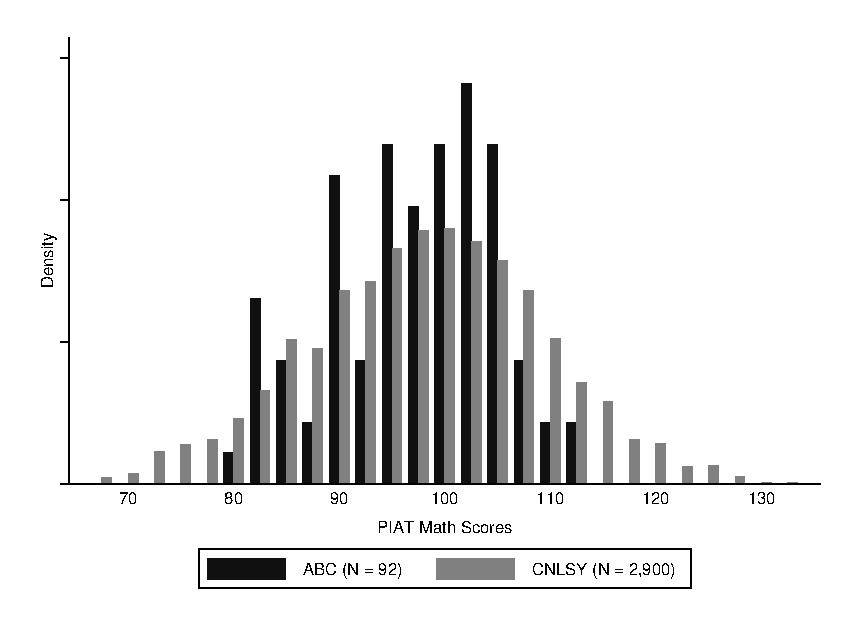
\includegraphics[width=\textwidth]{AppOutput/Methodology/support_math.eps}
	\end{subfigure}
	
	\begin{subfigure}[h]{0.8\textwidth}
	\centering
	\caption{Mother's Years of Education} \label{fig:support_meduc}
	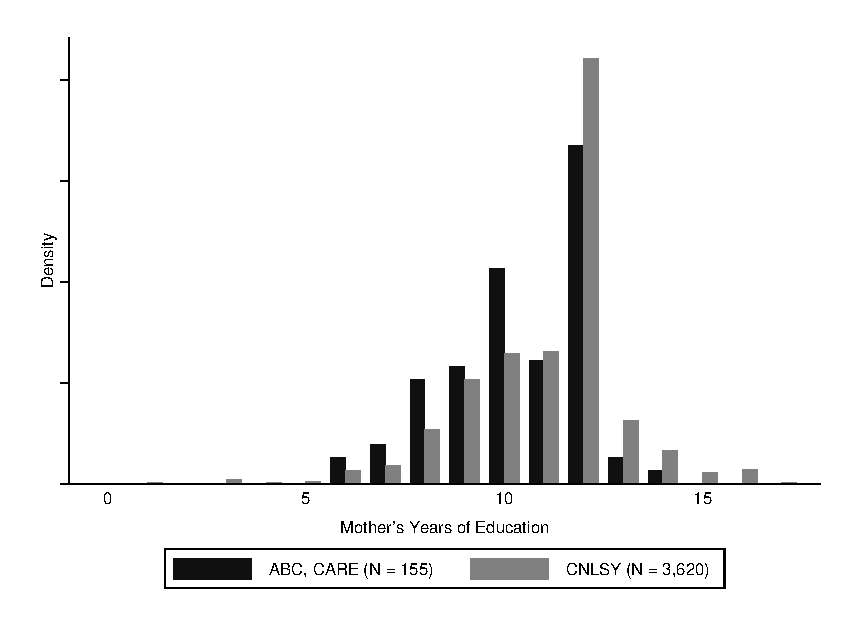
\includegraphics[width=\textwidth]{AppOutput/Methodology/support_momed.eps}
	\end{subfigure}
	
	\floatfoot{
	\footnotesize
	\noindent Note: These graphs display the support of ABC, PSID, NLSY79, and CNLSY
	for variables we use to forecast future labor income. PIAT math
	scores are averaged over ages 5--7.
	}
\end{figure}

\begin{figure}[H]
		\ContinuedFloat
	\begin{subfigure}[h]{0.8\textwidth}
	\centering
	\caption{Subject's Years of Education} \label{fig:support_educ}
	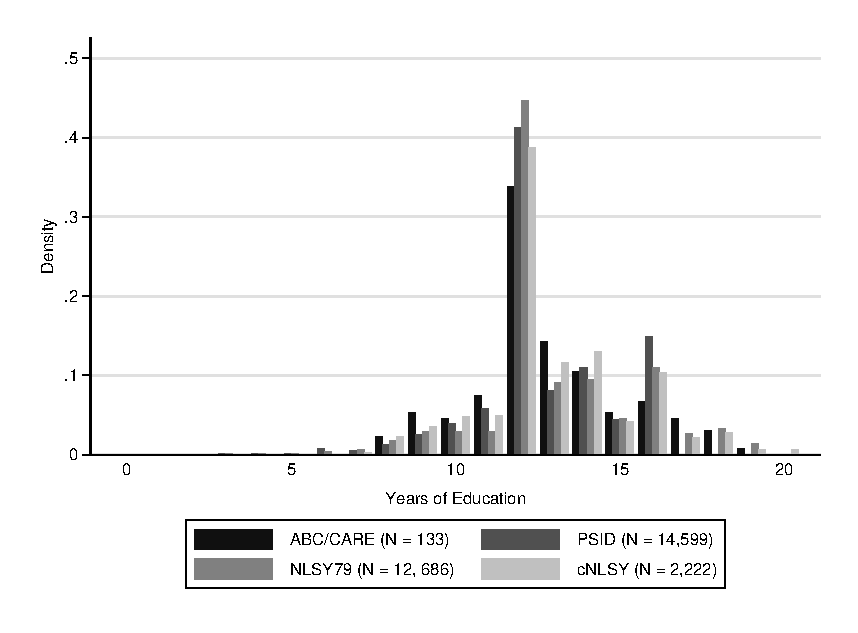
\includegraphics[width=\textwidth]{AppOutput/Methodology/support_educ.eps}
	\end{subfigure}
	
	\begin{subfigure}[h]{0.8\textwidth}
	\centering
	\caption{Income at Age 21} \label{fig:support_inc21}
	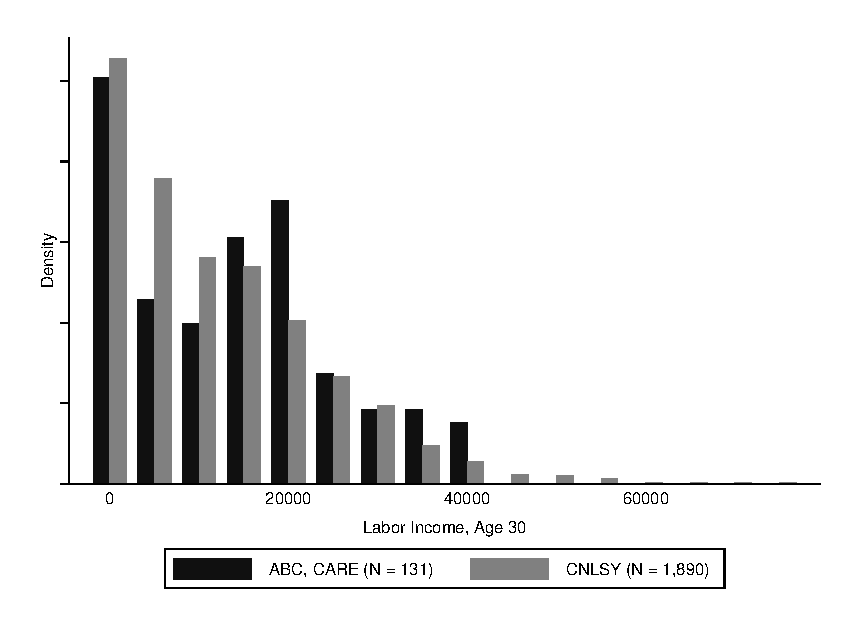
\includegraphics[width=\textwidth]{AppOutput/Methodology/support_inc21.eps}
	\end{subfigure}
	
\end{figure}

\begin{figure}[H]
	\ContinuedFloat
	
	\begin{subfigure}[h]{0.8\textwidth}
	\centering
	\caption{Income at Age 30} \label{fig:support_inc30}
	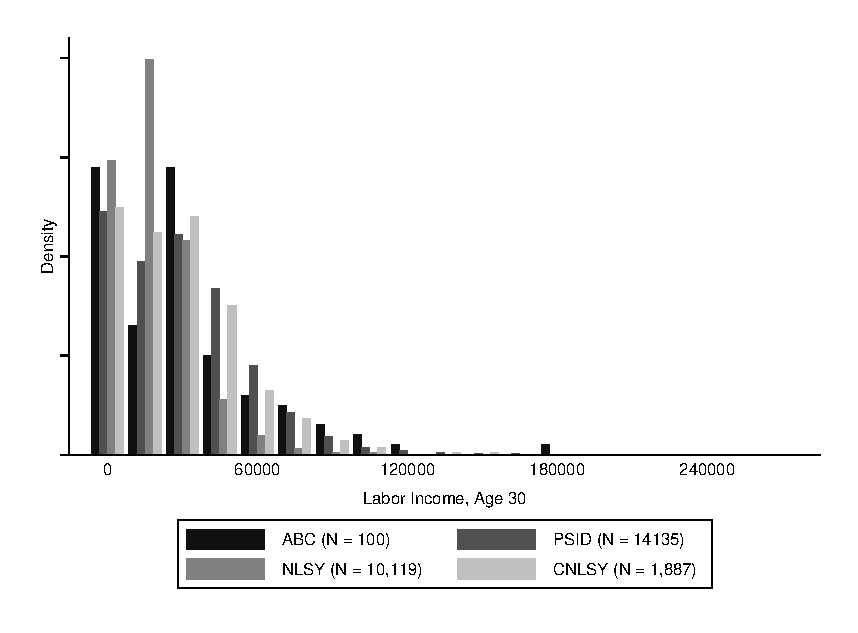
\includegraphics[width=\textwidth]{AppOutput/Methodology/support_inc30.eps}
	\end{subfigure}

	
	\begin{subfigure}[h]{0.8\textwidth}
	\centering
	\caption{Body Mass Index, Age 34} \label{fig:support_bmi}
	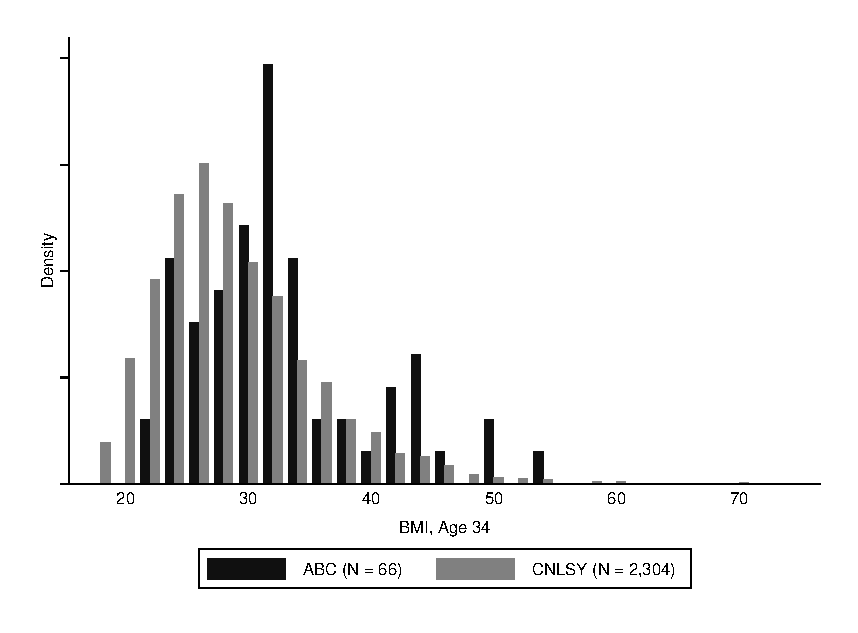
\includegraphics[width=\textwidth]{AppOutput/Methodology/support_bmi.eps}
	\end{subfigure}
	
\end{figure}

\subsubsection{Testing Assumption~\ref{ass:exog}: Exogeneity} \label{app:endogeneity}

\noindent The following framework helps us to test both Assumptions~\ref{ass:exog} and \ref{ass:summary}. We discuss this framework and test Assumption~\ref{ass:exog} in this section of the appendix. We test Assumption~\ref{ass:summary} in the next section.

\noindent Define an outcome vector for treatment status $d$, in sample $k$ at age $a$ as

\begin{align}
\bm{Y}^d_{k,a} &= \bm{X}^d_{k,a} \bm{\gamma} + \mathcal{E}^d_a  &(a) \nonumber
\end{align}

\noindent with an associated measurement system

\begin{align}  \label{eq:sa-msystemmain}
\mathcal{E}_{a}^d &=\bm{\beta}^d \bm{\theta}_{a}^d + \bm{\omega}_{a}^d  &(b) \nonumber \\
\bm{M}_{a}^d &= \bm{\lambda}^d \bm{\theta}_{a}^d + \bm{\upsilon}_a^d,  &(c)
\end{align}


\noindent where $\bm{\theta}^d \independent \bm{\upsilon}_{a}^d, \bm{\omega}_{a}^d$ and $\bm{\upsilon}_{a}^d \independent \bm{\omega}_{a}^d$. We use additional conditioning variables in these equations. To simplify the notation, we keep them implicit.

\noindent When the auxiliary measurement system $\bm{M}_{a}^d $ consists of at least three measures, we are able to identify the vectors of coefficients characterizing this system, $\bm{\lambda}^d, \bm{\beta}^d$, as well as the respective covariance matrices, $\bm{\Sigma}_{\bm{\theta}_{a}^d}, \bm{\Sigma}_{\bm{\upsilon}_{a}^d}, \bm{\Sigma}_{\bm{\omega}_{a}^d}$, we use the method from \citet{Bartlett_1938_Nature} to obtain an estimate of $\bm{\theta}_{a}^d$ \citep{Heckman_Pinto_etal_2013_PerryFactor}. Identifying and estimating the elements in system \eqref{eq:sa-msystemmain} serves two purposes: (i) it facilitates a test of Assumption~\ref{ass:exog}; and (ii) it enables us to use estimates of $\bm{\theta}_{a}^d$ as control functions when testing Assumption~\ref{ass:summary} in the next appendix, i.e. to use these estimates to control for endogeneity.

\noindent We first describe the estimates for the elements in System~\eqref{eq:sa-msystemmain} in the experimental sample. We assume that $\bm{\theta}_{a}^d$ has two dimensions (one representing cognitive skill, $c$, and another representing non-cognitive skill, $nc$). We assume dedicated measures for these skills at one time period. Put simply, we have two independent systems, one to measure $\bm{\theta}_{c}^d$ and one to measure $\bm{\theta}_{nc}^d$, where $\bm{\theta}_{a}^d: = \left[ \bm{\theta}_{c}^d, \bm{\theta}_{nc}^d \right]$. Further, we assume a common measurement system for the treatment and control groups (this is a sensible assumption shown to be true in the Perry data; see \citealp{Heckman_Pinto_etal_2013_PerryFactor}). This assumption implies that $\bm{\lambda}^d, \bm{\beta}^d$, as well as $\bm{\Sigma}_{\bm{\theta}_{a}^d}, \bm{\Sigma}_{\bm{\upsilon}_{a}^d}$ are the same whether $d = 0$ or $d = 1$.

\noindent We use a set of IQ measures from ages 2 to 8 to obtain an estimate of $\bm{\theta}_{c}^d$ and a set of measures of somatization, hostility, depression, and mental health all at age 21 to measure to estimate $\bm{\theta}_{nc}^d$.\footnote{For definitions and treatment effects on these variables see Appendix~\ref{appendix:results}.} Figure~\ref{figure:factorsm} shows our estimates by treatment status.

\begin{figure}[!htbp]
\centering
\caption{Estimates of Cognitive ($\theta_{c}^d$) and Non-cognitive Skills ($\theta_{nc}^d$)}\label{figure:factorsm}
\begin{subfigure}[h]{0.5\textwidth}
		\centering
		\caption{Cognitive} \label{fig:c}
		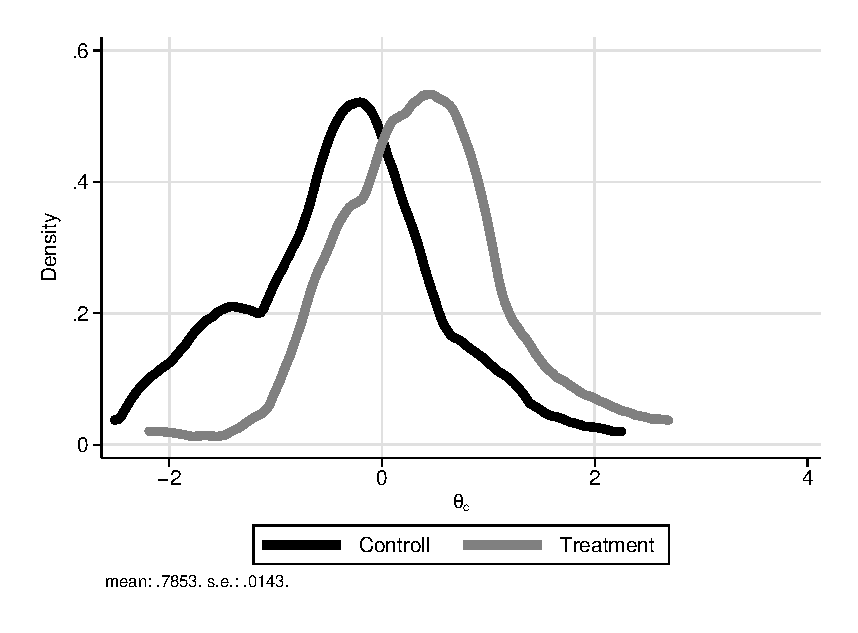
\includegraphics[width=\textwidth]{output/abccare_cfactor.eps}
\end{subfigure}%
\begin{subfigure}[h]{0.5\textwidth}
	\centering
	\caption{Non-cognitive} \label{fig:n}
		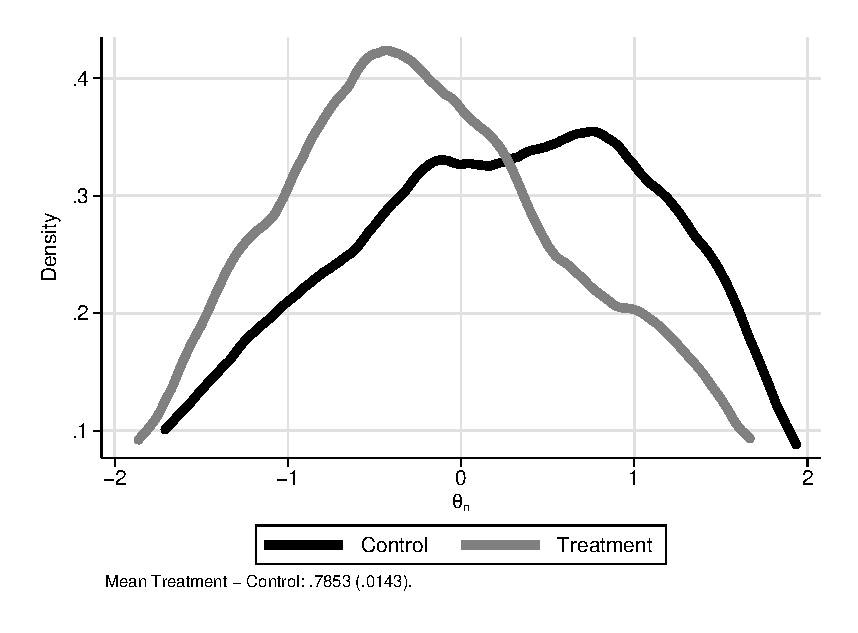
\includegraphics[width=\textwidth]{output/abccare_nfactor.eps}
\end{subfigure}
\footnotesize \justify
Note: Panel (a) displays a factor score estimated based on the measurement system in \eqref{eq:sa-msystemmain} and measures of IQ at ages 2, 3, 4, 5, 7, and 8 (cognitive skill). Panel (b) displays an analogous set of graphs for measures of somatization, hostility, depression, and mental health at age 21 (non-cognitive skill). Both measures of skills are standardized to a mean of $0$ and a standard deviation of $1$. ``Less'' in the factor measuring non-cognitive skills is ``positive'' given the measures we rely on to construct it. The mean difference between treatment and control is displayed below each panel, with standard error in parentheses. Standard errors are based on the empirical bootstrap distribution.
\end{figure}

\noindent We can also estimate $\bm{\theta}_{a}^d$ in the auxiliary sample. For want of data to approximate $\bm{\theta}_{c}, \bm{\theta}_{nc}$ in PSID and NLSY79, we use the CNLSY in this appendix. Our measurement system for $\bm{\theta}_{c}$ consists of reading and comprehension PIAT scores as well as by the Peabody Picture Vocabulary Test (PPVT). Our measurement system for $\bm{\theta}_{nc}$ is based on six scales of the Behavior Problems Index (e.g., anxiety, dependency, social behavior).

\noindent Once these estimates are available, we can test Assumption~\ref{ass:exog} in the experimental and auxiliary samples. The test consists of the following. Let $\bm{\gamma}^E$ be the parameter associated to $\bm{X}^d_{k,a}$ in Equation (a) in System~\eqref{eq:sa-msystemmain} when not accounting for $\bm{\theta}_{a}^d$. Similarly, let $\bm{\gamma}^I$ be the parameter associated with $\bm{X}^d_{k,a}$ in Equation (a) in System~\eqref{eq:sa-msystemmain} when accounting for $\bm{\theta}_{a}^d$. Under the null hypotheses, Assumption~\ref{ass:exog} holds and $\bm{\theta}_{a}^d$ is an irrelevant predictor in Equation (a) in System~\eqref{eq:sa-msystemmain}. This makes the OLS estimate of $\bm{\gamma}^E$ inconsistent. If the null hypotheses are false, $\bm{X}^d_{k,a}$ and $\varepsilon_{a}^d$ are not independent, $\bm{\gamma}^I$ is consistent and $\bm{\gamma}^E$ is not. We test the null hypothesis by asking if the elements in $\bm{\theta}_{a}^d$ are relevant predictors of a set of outcomes at age 30, so that we can perform the tests on both the experimental and the auxiliary samples. We contrast specifications with and without including estimates of $\bm{\theta}_{a}^d$, and report the $F$-statistic corresponding to this comparison. This is a version of a Durbin-Wu-Hausman test \citep[see][]{Durbin_1954_RISI,Wu_1973_Econometrica,Hausman_1978_Econometrica}. Tables~\ref{table:endoginc} to \ref{table:trincome} present the results. In most cases, we are not able to reject the null hypothesis that Assumption~\ref{ass:exog} holds.


\begin{sidewaystable}[H]
\begin{threeparttable}
\caption{Forecast of Labor Income at Age 30 Accounting for $\bm{B}_k$ and $\bm{\theta}, \bm{X}_{k,a}$, ABC/CARE Control Group}
\label{table:endoginc}
\centering
\footnotesize
\begin{tabular}{lcccccccc} \toprule
 & (1) & (2) & (3) & (4) & (5) & (6) & (7) & (8) \\
 & Estimate & $p$-value & Estimate & $p$-value  & Estimate & $p$-value  & Estimate & $p$-value  \\ \midrule 
Mother's Education &     1,599.57 &         0.17 &       867.41 &         0.34 &      -769.20 &         0.68 &      -580.88 &         0.62 \\  
PIAT (5-7) &            . &            . &            . &            . &        45.98 &         0.41 &       423.44 &         0.20 \\  
Education (30) &            . &            . &            . &            . &     3,415.53 &         0.03 &     4,505.94 &         0.04 \\  
Labor Income (21) &            . &            . &            . &            . &         0.69 &         0.02 &         0.97 &         0.03 \\  
Cognitive &            . &            . &       758.28 &         0.43 &            . &            . &    -8,009.28 &         0.93 \\  
Non Cognitive &            . &            . &      -342.62 &         0.52 &            . &            . &     7,275.49 &         0.09 \\  
Constant &    10,239.82 &         0.28 &    16,530.50 &         0.22 &   -23,140.28 &         0.80 &   -80,679.09 &         0.96 \\  \\ \midrule
R2 &         \multicolumn{2}{c}{0.03} &              \multicolumn{2}{c}{0.07} &             \multicolumn{2}{c}{0.30} &               \multicolumn{2}{c}{0.40}  \\  
Observations &         \multicolumn{2}{c}{66} &          \multicolumn{2}{c}{51} &              \multicolumn{2}{c}{65} &             \multicolumn{2}{c}{63}  \\  \\ \midrule
$F$-stat: exclude Cognitive, Non-Cognitive &              \multicolumn{4}{c}{1.70} &               \multicolumn{4}{c}{4.14}  \\  
$p$-value  &         \multicolumn{4}{c}{0.45} &                   \multicolumn{4}{c}{0.09} \\      \bottomrule \end{tabular}


\begin{tablenotes}
\footnotesize
\item $F$-stat: exclude Cognitive and Non-Cognitive: $F$-statistic contrasting the specifications in columns (1) and (3) and (5) and (7), respectively.\\
\item Note: Forecast of labor income at age 30 is based on the variable listed in the row. Empty cells indicate that the variable was not used in the prediction. For each coefficient we provide the point estimate and $p$-value for the treatment and control groups as well as a test for the treatment-control difference. $\hat{\bm{\theta}}_{c}$: factor score estimated based on the measurement system in \eqref{eq:sa-msystemmain} and measures of IQ at ages 2, 3, 4, 5, 7, and 8 (cognitive skill). $\hat{\bm{\theta}}_{n}$: factor score estimated based on the measurement system in \eqref{eq:sa-msystemmain} and measures of somatization, hostility, depression, and a global mental health index at age 21 (non-cognitive skill). Both measures of skills are standardized to a mean of $0$ and a standard deviation of $1$. Inference is based on the empirical bootstrap distribution. If the estimates for the constant terms are in the ten or hundred thousands, we report a figure that has been rounded to the thousands.
\end{tablenotes}
\end{threeparttable}
\end{sidewaystable}

\begin{sidewaystable}[H]
\begin{threeparttable}
\caption{Forecast of Labor Income at Age 30 Accounting for $\bm{B}_k$ and $\bm{\theta}, \bm{X}_{k,a}$, ABC/CARE Treatment Group}
\centering
\footnotesize
\begin{tabular}{lcccccccc} \toprule
 & (1) & (2) & (3) & (4) & (5) & (6) & (7) & (8) \\
 & Estimate & $p$-value & Estimate & $p$-value  & Estimate & $p$-value  & Estimate & $p$-value  \\ \midrule 
Mother's Education &     3,134.16 &         0.23 &     2,600.34 &         0.35 &     2,913.44 &         0.28 &     5,835.67 &         0.22 \\  
PIAT (5-7) &            . &            . &            . &            . &      -263.29 &         0.66 &      -871.06 &         0.76 \\  
Education (30) &            . &            . &            . &            . &    11,600.24 &         0.00 &    13,069.48 &         0.00 \\  
Labor Income (21) &            . &            . &            . &            . &        -0.18 &         0.64 &        -0.62 &         0.75 \\  
Cognitive &            . &            . &     2,766.35 &         0.40 &            . &            . &     4,828.93 &         0.34 \\  
Non Cognitive &            . &            . &     7,600.33 &         0.18 &            . &            . &     6,223.32 &         0.19 \\  
Constant &     3,900.73 &         0.47 &    10,553.93 &         0.42 &  -122,709.85 &         0.91 &  -109,410.81 &         0.76 \\  \\ \midrule
$R^2$ &         \multicolumn{2}{c}{0.02} &          \multicolumn{2}{c}{0.10} &          \multicolumn{2}{c}{0.26} &             \multicolumn{2}{c}{0.33} \\ 
Observations &         \multicolumn{2}{c}{64} &         \multicolumn{2}{c}{49} &                \multicolumn{2}{c}{65} &       \multicolumn{2}{c}{63}  \\   \\ \midrule
$F$-stat: exclude Cognitive, Non-Cognitive &             \multicolumn{4}{c}{3.13} &              \multicolumn{4}{c}{2.14}  \\  
$p$-value &                 \multicolumn{4}{c}{0.27} &                   \multicolumn{4}{c}{0.27}  \\    \bottomrule \end{tabular}


\begin{tablenotes}
\footnotesize
\item $F$-stat: exclude Cognitive and Non-Cognitive: $F$-statistic contrasting the specifications in columns (1) and (3) and (5) and (7), respectively.\\
\item Note: Forecast of labor income at age 30 is based on the variable listed in the row. Empty cells indicate that the variable was not used in the prediction. For each coefficient we provide the point estimate and $p$-value for the treatment and control groups as well as a test for the treatment-control difference. $\hat{\bm{\theta}}_{c}$: factor score estimated based on the measurement system in \eqref{eq:sa-msystemmain} and measures of IQ at ages 2, 3, 4, 5, 7, and 8 (cognitive skill). $\hat{\bm{\theta}}_{n}$: factor score estimated based on the measurement system in \eqref{eq:sa-msystemmain} and measures of somatization, hostility, depression, and a global mental health index at age 21 (non-cognitive skill). Both measures of skills are standardized to a mean of $0$ and a standard deviation of $1$. Inference is based on the empirical bootstrap distribution. If the estimates for the constant terms are in the ten or hundred thousands, we report a figure that has been rounded to the thousands.
\end{tablenotes}
\end{threeparttable}
\end{sidewaystable}

\begin{sidewaystable}[H]
\begin{threeparttable}
\caption{Forecast of Labor Income at Age 30 Accounting for $\bm{B}_k$ and $\bm{\theta}, \bm{X}_{k,a}$, ABC/CARE Control and Treatment Groups}
\centering
\footnotesize
\begin{tabular}{lcccccccc} \toprule
 & (1) & (2) & (3) & (4) & (5) & (6) & (7) & (8) \\
 & Estimate & $p$-value & Estimate & $p$-value  & Estimate & $p$-value  & Estimate & $p$-value  \\ \midrule 
Mother's Education &     2,668.48 &         0.12 &     2,200.35 &         0.25 &       794.11 &         0.36 &     1,724.88 &         0.31 \\  
PIAT (5-7) &            . &            . &            . &            . &      -126.19 &         0.67 &      -400.57 &         0.72 \\  
Education (30) &            . &            . &            . &            . &     8,601.33 &         0.00 &     9,706.02 &         0.00 \\  
Labor Income (21) &            . &            . &            . &            . &         0.14 &         0.37 &         0.21 &         0.37 \\  
Cognitive &            . &            . &     4,260.39 &         0.16 &            . &            . &     1,427.18 &         0.44 \\  
Non Cognitive &            . &            . &     2,899.66 &         0.25 &            . &            . &     7,557.01 &         0.05 \\  
Constant &     4,443.37 &         0.41 &     9,166.30 &         0.38 &   -78,053.28 &         0.95 &   -75,621.84 &         0.87 \\  \\ \midrule
$R^2$ &         \multicolumn{2}{c}{0.02} &          \multicolumn{2}{c}{0.04} &             \multicolumn{2}{c}{0.20} &                 \multicolumn{2}{c}{0.25}  \\  
Observations &        \multicolumn{2}{c}{132} &        \multicolumn{2}{c}{100} &     \multicolumn{2}{c}{130} &         \multicolumn{2}{c}{133}  \\  \\ \midrule
$F$-stat: exclude Cognitive, Non-Cognitive  &             \multicolumn{4}{c}{2.07} &               \multicolumn{4}{c}{2.92}  \\  
$p$-value &                \multicolumn{4}{c}{0.31} &               \multicolumn{4}{c}{0.19}   \\  \bottomrule \end{tabular}
\begin{tablenotes}
\footnotesize
\item $F$-stat: exclude Cognitive and Non-Cognitive: $F$-statistic contrasting the specifications in columns (1) and (3) and (5) and (7), respectively.\\
\item Note: Forecast of labor income at age 30 is based on the variable listed in the row. Empty cells indicate that the variable was not used in the prediction. For each coefficient we provide the point estimate and $p$-value for the treatment and control groups as well as a test for the treatment-control difference.  $\hat{\bm{\theta}}_{c}$: factor score estimated based on the measurement system in \eqref{eq:sa-msystemmain} and measures of IQ at ages 2, 3, 4, 5, 7, and 8 (cognitive skill). $\hat{\bm{\theta}}_{n}$: factor score estimated based on the measurement system in \eqref{eq:sa-msystemmain} and measures of somatization, hostility, depression, and a global mental health index at age 21 (non-cognitive skill). Both measures of skills are standardized to a mean of $0$ and a standard deviation of $1$. Inference is based on the empirical bootstrap distribution. If the estimates for the constant terms are in the ten or hundred thousands, we report a figure that has been rounded to the thousands.
\end{tablenotes}
\end{threeparttable}
\end{sidewaystable}

\begin{sidewaystable}[H]
\begin{threeparttable}
\caption{Forecast of Labor Income at Age 30 Accounting for $\bm{B}_k$ and $\bm{\theta}, \bm{X}_{k,a}$, CNLSY}
\centering
\footnotesize
\begin{tabular}{lcccccccc} \toprule
 & (1) & (2) & (3) & (4) & (5) & (6) & (7) & (8) \\
 & Estimate & $p$-value & Estimate & $p$-value  & Estimate & $p$-value  & Estimate & $p$-value  \\ \midrule 
Mother's Education &     2,317.52 &         0.00 &     2,262.79 &         0.00 &       316.78 &         0.23 &       379.54 &         0.32 \\  
PIAT (5-7) &            . &            . &            . &            . &       263.98 &         0.00 &       471.53 &         0.00 \\  
Education (30) &            . &            . &            . &            . &     3,647.75 &         0.00 &     4,351.32 &         0.00 \\  
Labor Income (21) &            . &            . &            . &            . &         0.68 &         0.00 &         0.79 &         0.00 \\  
Cognitive &            . &            . &     2,680.61 &         0.13 &            . &            . &    -4,541.18 &         0.95 \\  
Non Cognitive &            . &            . &    -3,584.83 &         0.99 &            . &            . &    -1,352.32 &         0.79 \\  
Constant &     2,523.10 &         0.25 &     3,699.61 &         0.37 &   -56,008.30 &         1.00 &   -86,767.50 &         1.00 \\ \\ \midrule
$R^2$ &         \multicolumn{2}{c}{0.03} &              \multicolumn{2}{c}{0.06} &               \multicolumn{2}{c}{0.21} &                \multicolumn{2}{c}{0.34}  \\  
Observations &       \multicolumn{2}{c}{1,885} &            \multicolumn{2}{c}{370} &           \multicolumn{2}{c}{1,885} &          \multicolumn{2}{c}{1,883}   \\  \\ \midrule
$F$-stat: exclude Cognitive, Non-Cognitive &                      \multicolumn{4}{c}{1.28} &                      \multicolumn{4}{c}{4.93}   \\  
$p$-value &             \multicolumn{4}{c}{0.44} &                  \multicolumn{4}{c}{0.44}  \\    \bottomrule \end{tabular}

\begin{tablenotes}
\footnotesize
\item $F$-stat: exclude Cognitive and Non-Cognitive: $F$-statistic contrasting the specifications in columns (1) and (3) and (5) and (7), respectively.\\
\item Note: Forecast of labor income at age 30 is based on the variable listed in the row. Empty cells indicate that the variable was not used in the prediction. For each coefficient we provide the point estimate and $p$-value for the treatment and control groups as well as a test for the treatment-control difference. $\hat{\bm{\theta}}_{c}$: factor score estimated based on the measurement system in \eqref{eq:sa-msystemmain} and measures of reading and comprehension of the PIAT, as weel as the Peabody Picture Vocabulary Test (PPVT) (cognitive skill). $\hat{\bm{\theta}}_{n}$: factor score estimated based on the measurement system in \eqref{eq:sa-msystemmain} and six scales of the Behavior Problems Index (e.g., anxiety, dependency, social behavior) (non-cognitive skill). Both measures of skills are standardized to a mean of $0$ and a standard deviation of $1$. Inference is based on the empirical bootstrap distribution. If the estimates for the constant terms are in the ten or hundred thousands, we report a figure that has been rounded to the thousands.
\end{tablenotes}
\end{threeparttable}
\end{sidewaystable}

\begin{sidewaystable}[H]
\begin{threeparttable}
\caption{Forecast of Transfer Income at Age 30 Accounting for $\bm{B}_k$ and $\bm{\theta}, \bm{X}_{k,a}$, ABC/CARE Control Group}
\label{table:endoginc}
\centering
\footnotesize
\begin{tabular}{lcccccccc} \toprule
 & (1) & (2) & (3) & (4) & (5) & (6) & (7) & (8) \\
 & Estimate & $p$-value & Estimate & $p$-value  & Estimate & $p$-value  & Estimate & $p$-value  \\ \midrule 
Mother's Education &      -413.76 &         0.78 &      -406.14 &         0.69 &        48.75 &         0.49 &        51.97 &         0.47 \\  
PIAT (5-7) &            . &            . &            . &            . &        27.10 &         0.29 &      -101.93 &         0.77 \\  
Education (30) &            . &            . &            . &            . &      -684.75 &         0.99 &      -693.44 &         0.91 \\  
Labor Income (21) &            . &            . &            . &            . &        -0.14 &         0.99 &        -0.15 &         0.93 \\  
Cognitive &            . &            . &      -348.53 &         0.69 &            . &            . &     1,696.96 &         0.13 \\  
Non Cognitive &            . &            . &     1,622.92 &         0.05 &            . &            . &       887.17 &         0.19 \\  
Constant &     6,664.39 &         0.11 &     6,614.39 &         0.18 &     9,942.56 &         0.18 &    22,736.59 &         0.10 \\  \\ \midrule 
$F$-stat &          \multicolumn{2}{c}{1.93} &             \multicolumn{2}{c}{2.96} &            \multicolumn{2}{c}{3.53} &              \multicolumn{2}{c}{2.68}   \\  
$p$-value &          \multicolumn{2}{c}{0.34} &             \multicolumn{2}{c}{0.15} &            \multicolumn{2}{c}{0.21} &              \multicolumn{2}{c}{0.27}   \\  
$R^2$ &          \multicolumn{2}{c}{0.04} &             \multicolumn{2}{c}{0.15} &            \multicolumn{2}{c}{0.21} &              \multicolumn{2}{c}{0.27}   \\  
Observations &         \multicolumn{2}{c}{68} &                 \multicolumn{2}{c}{52} &               \multicolumn{2}{c}{70}  &                \multicolumn{2}{c}{70}   \\  \\ \midrule
$F$-stat: exclude Cognitive, Non-Cognitive  &                 \multicolumn{4}{c}{3.38} &              \multicolumn{4}{c}{2.42}  \\  
$p$-value &                \multicolumn{4}{c}{0.19} &               \multicolumn{4}{c}{0.27}  \\      \bottomrule \end{tabular}
\begin{tablenotes}
\footnotesize
\item $F$-stat: exclude Cognitive and Non-Cognitive: $F$-statistic contrasting the specifications in columns (1) and (3) and (5) and (7), respectively.\\
\item Note: Forecast of labor income at age 30 is based on the variable listed in the row. Empty cells indicate that the variable was not used in the prediction. For each coefficient we provide the point estimate and $p$-value for the treatment and control groups as well as a test for the treatment-control difference. $\hat{\bm{\theta}}_{c}$: factor score estimated based on the measurement system in \eqref{eq:sa-msystemmain} and measures of IQ at ages 2, 3, 4, 5, 7, and 8 (cognitive skill). $\hat{\bm{\theta}}_{n}$: factor score estimated based on the measurement system in \eqref{eq:sa-msystemmain} and measures of somatization, hostility, depression, and a global mental health index at age 21 (non-cognitive skill). Both measures of skills are standardized to a mean of $0$ and a standard deviation of $1$. Inference is based on the empirical bootstrap distribution. If the estimates for the constant terms are in the ten or hundred thousands, we report a figure that has been rounded to the thousands.
\end{tablenotes}
\end{threeparttable}
\end{sidewaystable}

\begin{sidewaystable}[H]
\begin{threeparttable}
\caption{Forecast of Transfer Income at Age 30 Accounting for $\bm{B}_k$ and $\bm{\theta}, \bm{X}_{k,a}$, ABC/CARE Treatment Group}
\centering
\footnotesize
\begin{tabular}{lcccccccc} \toprule
 & (1) & (2) & (3) & (4) & (5) & (6) & (7) & (8) \\
 & Estimate & $p$-value & Estimate & $p$-value  & Estimate & $p$-value  & Estimate & $p$-value  \\ \midrule 
Mother'sEducation &      -212.39 &         0.75 &      -336.44 &         0.81 &      -199.39 &         0.74 &      -302.60 &         0.79 \\  
PIAT(5-7) &            . &            . &            . &            . &       -46.36 &         0.86 &       -22.41 &         0.65 \\  
Education(30) &            . &            . &            . &            . &       -35.62 &         0.56 &       -72.66 &         0.59 \\  
LaborIncome(21) &            . &            . &            . &            . &        -0.05 &         0.94 &        -0.05 &         0.90 \\  
Cognitive &            . &            . &      -421.59 &         0.75 &            . &            . &      -273.48 &         0.62 \\  
Non Cognitive &            . &            . &      -825.26 &         0.95 &            . &            . &      -987.11 &         0.98 \\  
Constant &     3,348.22 &         0.16 &     4,937.75 &         0.14 &     9,041.98 &         0.09 &     8,432.47 &         0.18 \\  \\ \midrule
$R^2$  &          \multicolumn{2}{c}{0.03} &            \multicolumn{2}{c}{0.15} &                  \multicolumn{2}{c}{0.13} &               \multicolumn{2}{c}{0.25}  \\  
Observations &        \multicolumn{2}{c}{63} &               \multicolumn{2}{c}{49}  &             \multicolumn{2}{c}{65}  &         \multicolumn{2}{c}{63}  \\   \\ \midrule
$F$-stat: exclude Cognitive, Non-Cognitive &                    \multicolumn{4}{c}{4.15} &                   \multicolumn{4}{c}{2.90}  \\  
$p$-value &              \multicolumn{4}{c}{0.28} &                    \multicolumn{4}{c}{0.28}  \\      \bottomrule \end{tabular}
\begin{tablenotes}
\footnotesize
\item $F$-stat: exclude Cognitive and Non-Cognitive: $F$-statistic contrasting the specifications in columns (1) and (3) and (5) and (7), respectively.\\
\item Note: Forecast of labor income at age 30 is based on the variable listed in the row. Empty cells indicate that the variable was not used in the prediction. For each coefficient we provide the point estimate and $p$-value for the treatment and control groups as well as a test for the treatment-control difference. $\hat{\bm{\theta}}_{c}$: factor score estimated based on the measurement system in \eqref{eq:sa-msystemmain} and measures of IQ at ages 2, 3, 4, 5, 7, and 8 (cognitive skill). $\hat{\bm{\theta}}_{n}$: factor score estimated based on the measurement system in \eqref{eq:sa-msystemmain} and measures of somatization, hostility, depression, and a global mental health index at age 21 (non-cognitive skill). Both measures of skills are standardized to a mean of $0$ and a standard deviation of $1$. Inference is based on the empirical bootstrap distribution. If the estimates for the constant terms are in the ten or hundred thousands, we report a figure that has been rounded to the thousands.
\end{tablenotes}
\end{threeparttable}
\end{sidewaystable}

\begin{sidewaystable}[H]
\begin{threeparttable}
\caption{Forecast of Transfer Income at Age 30 Accounting for $\bm{B}_k$ and $\bm{\theta}, \bm{X}_{k,a}$, ABC/CARE Control and Treatment Groups}
\centering
\footnotesize
\begin{tabular}{lcccccccc} \toprule
 & (1) & (2) & (3) & (4) & (5) & (6) & (7) & (8) \\
 & Estimate & $p$-value & Estimate & $p$-value  & Estimate & $p$-value  & Estimate & $p$-value  \\ \midrule 
Mother's Education &      -299.72 &         0.81 &      -411.12 &         0.85 &      -135.23 &         0.62 &      -211.76 &         0.68 \\  
PIAT (5-7) &            . &            . &            . &            . &       -34.90 &         0.81 &       -66.99 &         0.80 \\  
Education (30) &            . &            . &            . &            . &      -430.88 &         0.96 &      -453.82 &         0.96 \\  
Labor Income (21) &            . &            . &            . &            . &        -0.09 &         1.00 &        -0.08 &         0.96 \\  
Cognitive &            . &            . &      -753.98 &         0.93 &            . &            . &       153.54 &         0.42 \\  
Non Cognitive &            . &            . &       631.74 &         0.17 &            . &            . &       264.49 &         0.34 \\  
Constant &     5,135.83 &         0.06 &     6,460.15 &         0.07 &    13,548.68 &         0.03 &    17,791.02 &         0.05 \\   \\ \midrule
$F$-stat &         \multicolumn{2}{c}{1.78} &         \multicolumn{2}{c}{3.04} &               \multicolumn{2}{c}{3.86} &            \multicolumn{2}{c}{2.75}  \\  
$p$-value &         \multicolumn{2}{c}{0.35} &         \multicolumn{2}{c}{0.12} &               \multicolumn{2}{c}{0.35} &            \multicolumn{2}{c}{0.09}  \\  
$R^2$ &         \multicolumn{2}{c}{0.02} &         \multicolumn{2}{c}{0.10} &               \multicolumn{2}{c}{0.15} &            \multicolumn{2}{c}{0.18}  \\  
Observations &       \multicolumn{2}{c}{133} &           \multicolumn{2}{c}{101} &         \multicolumn{2}{c}{135} &            \multicolumn{2}{c}{133}  \\  \\ \midrule
$F$-stat: exclude Cognitive, Non-Cognitive &              \multicolumn{4}{c}{3.38} &             \multicolumn{4}{c}{1.23}  \\  
$p$-value &            \multicolumn{4}{c}{0.17} &               \multicolumn{4}{c}{0.44}  \\   \bottomrule \end{tabular}


\begin{tablenotes}
\footnotesize
\item $F$-stat: exclude Cognitive and Non-Cognitive: $F$-statistic contrasting the specifications in columns (1) and (3) and (5) and (7), respectively.\\
\item Note: Forecast of labor income at age 30 is based on the variable listed in the row. Empty cells indicate that the variable was not used in the prediction. For each coefficient we provide the point estimate and $p$-value for the treatment and control groups as well as a test for the treatment-control difference. $\hat{\bm{\theta}}_{c}$: factor score estimated based on the measurement system in \eqref{eq:sa-msystemmain} and measures of IQ at ages 2, 3, 4, 5, 7, and 8 (cognitive skill). $\hat{\bm{\theta}}_{n}$: factor score estimated based on the measurement system in \eqref{eq:sa-msystemmain} and measures of somatization, hostility, depression, and a global mental health index at age 21 (non-cognitive skill). Both measures of skills are standardized to a mean of $0$ and a standard deviation of $1$. Inference is based on the empirical bootstrap distribution. If the estimates for the constant terms are in the ten or hundred thousands, we report a figure that has been rounded to the thousands.
\end{tablenotes}
\end{threeparttable}
\end{sidewaystable}

\begin{sidewaystable}[H]
\begin{threeparttable}
\caption{Forecast of Transfer Income at Age 30 Accounting for $\bm{B}_k$ and $\bm{\theta}, \bm{X}_{k,a}$, CNLSY} \label{table:trincome}
\centering
\footnotesize
\begin{tabular}{lcccccccc} \toprule
 & (1) & (2) & (3) & (4) & (5) & (6) & (7) & (8) \\
 & Estimate & $p$-value & Estimate & $p$-value  & Estimate & $p$-value  & Estimate & $p$-value  \\ \midrule 
Mother'sEducation &      -457.46 &         0.56 &     8,259.13 &         0.04 &       985.13 &         0.41 &     9,344.69 &         0.02 \\  
PIAT(5-7) &            . &            . &            . &            . &      -273.46 &         0.64 &      -506.25 &         0.70 \\  
Education(30) &            . &            . &            . &            . &    -7,235.35 &         0.96 &    -5,622.52 &         0.84 \\  
LaborIncome(21) &            . &            . &            . &            . &         0.17 &         0.40 &        -0.96 &         0.98 \\  
Cognitive &            . &            . &    -8,525.66 &         0.83 &            . &            . &      -473.24 &         0.52 \\  
NonCognitive &            . &            . &    18,373.65 &         0.03 &            . &            . &     6,585.57 &         0.22 \\  
Constant &    34,777.07 &         0.14 &   -58,507.25 &         0.91 &   137,947.14 &         0.14 &    57,813.64 &         0.35 \\  \\ \midrule
$R^2$ &         \multicolumn{2}{c}{0.00} &               \multicolumn{2}{c}{0.02} &                \multicolumn{2}{c}{0.01} &             \multicolumn{2}{c}{0.05}   \\  
Observations &       \multicolumn{2}{c}{1,145} &              \multicolumn{2}{c}{244}  &       \multicolumn{2}{c}{1,145} &      \multicolumn{2}{c}{1,148}   \\  \\ \midrule
$F$-stat: exclude Cognitive, Non-Cognitive &                \multicolumn{4}{c}{1.86} &                 \multicolumn{4}{c}{1.03}   \\  
$p$-value  &                \multicolumn{4}{c}{0.23} &                \multicolumn{4}{c}{0.45}    \\  \bottomrule \end{tabular}


\begin{tablenotes}
\footnotesize
\item $F$-stat: exclude Cognitive and Non-Cognitive: $F$-statistic contrasting the specifications in columns (1) and (3) and (5) and (7), respectively.\\
\item Note: Forecast of labor income at age 30 is based on the variable listed in the row. Empty cells indicate that the variable was not used in the prediction. For each coefficient we provide the point estimate and $p$-value for the treatment and control groups as well as a test for the treatment-control difference. $\hat{\bm{\theta}}_{c}$: factor score estimated based on the measurement system in \eqref{eq:sa-msystemmain} and measures of reading and comprehension of the PIAT, as well as the Peabody Picture Vocabulary Test (PPVT) (cognitive skill). $\hat{\bm{\theta}}_{n}$: factor score estimated based on the measurement system in \eqref{eq:sa-msystemmain} and six scales of the Behavior Problems Index (e.g., anxiety, dependency, social behavior) (non-cognitive skill).  Both measures of skills are standardized to a mean of $0$ and a standard deviation of $1$. Inference is based on the empirical bootstrap distribution. If the estimates for the constant terms are in the ten or hundred thousands, we report a figure that has been rounded to the thousands.
\end{tablenotes}
\end{threeparttable}
\end{sidewaystable}

\subsubsection{Parental Labor Income}\label{app:parentalincome}

\noindent A substantial fraction of the ABC/CARE benefits come from parental labor income. The program operated as a childcare center, as well as a child development center. The parents were usually mothers: only $27\%$ of the mothers lived with a partner at baseline and there is little change in this status after enrollment. ABC/CARE relaxed the time constraint of the mothers, enabling them to educate themselves more and/or work more. The program had treatment effects on (i) maternal education; (ii) maternal labor supply; and (iii) maternal income.\footnote{See Appendix~\ref{appendix:results}.} Quantifying the effect of ABC/CARE on parental labor income requires quantifying its effects beyond age 5, after the subjects entered school. The program could have shifted the labor income profile through education or work experience. To test this, we need to quantify the effect that the program had from when it started until the mothers retired.

\noindent There are three options for monetizing parental labor income. (i) A conservative approach that we follow in the main text uses the available information and calculates the treatment effect of the program on labor income from ages 0 to 21. We observe parental labor income at ages 0, 1.5, 3.5, 4.5, 8, 12, 15, and 21. We interpolate between the ages that we observe and stop at age 21. The average age of the mothers at baseline was 21. On average, then, we omit 19 years of labor income if the mothers decide to retire at 60, 24 if they retire at 67, etc. (ii) A second approach is to use the available data together with an auxiliary sample to parameterize parental labor income when the subjects are older than 21. (iii) A third approach is to follow a similar methodology as the one we use for the subjects' labor and transfer income, making some adaptations given data limitations. Option (i) is straightforward. We explain options (ii) and (iii) next.

\noindent We note that the childcare feature of the program likely benefits parents who, at baseline, did not have any other children. If they did have other children, parents would still have to take care of the other children, weakening the childcare-driven effect on labor income (especially if there are younger siblings present). Figure~\ref{figure:pincome} shows that the net increase (treatment minus control) in discounted parental labor income is much higher in the absence of siblings (of the participant children) at baseline, using the ``conservative approach'' described above. The effect also weakens when comparing the outcomes of mothers whose children have siblings younger than 5 years old to the outcomes of mothers of children who have siblings 5 years old or younger.\footnote{These patterns persist when splitting the ABC/CARE sample by gender, but the estimates are not precise because the samples become too small.}

\begin{figure}[!htbp]
\centering
\caption{Discounted Net Present Value of Parental Labor Income by Participant's Number and Age of Siblings at Baseline}\label{figure:pincome}
\begin{subfigure}[h]{0.5\textwidth}
		\centering
		\caption{No Siblings vs. $>0$ Siblings}
		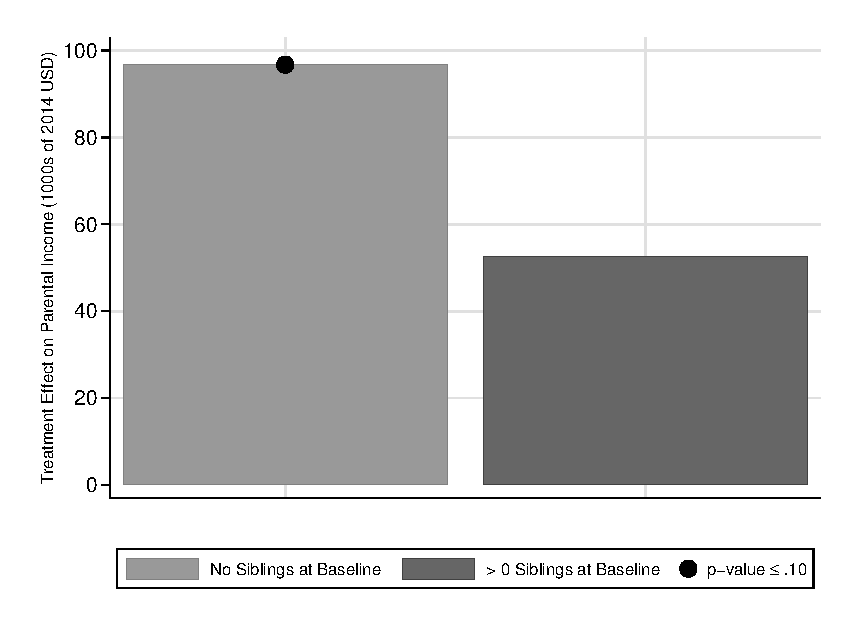
\includegraphics[width=\textwidth]{output/abccare_pincomesum_spooled.eps}
\end{subfigure}%
\begin{subfigure}[h]{0.5\textwidth}
		\centering
		\caption{Siblings Younger than 5 vs. Siblings 5 or Older}
		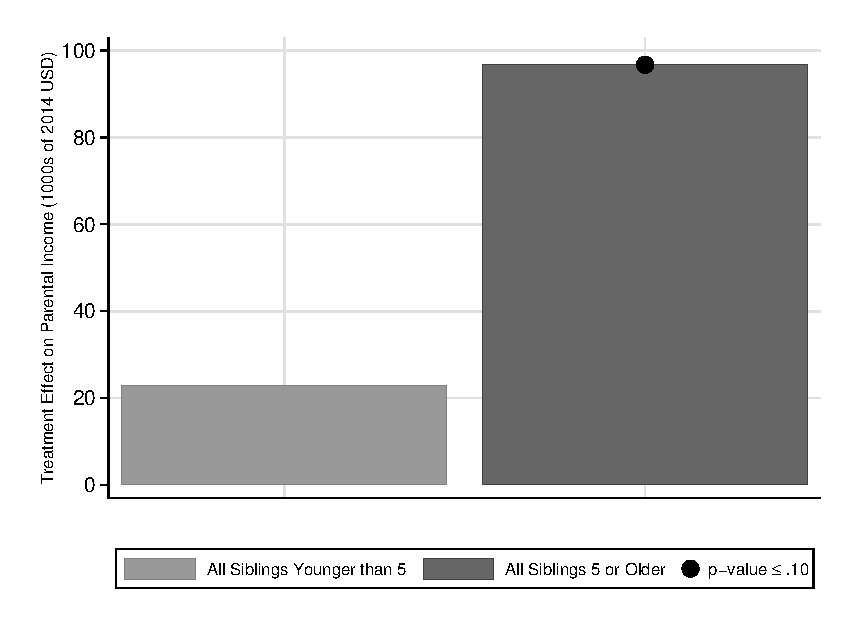
\includegraphics[width=\textwidth]{output/abccare_pincomesumsibage_spooled.eps}
\end{subfigure}
\footnotesize \justify
Note: Panel (a) displays the net-present value (treatment less control) of parental labor income of parents of children with and without siblings at baseline. Panel (b) displays the average parental labor income of parents of children with young siblings (younger than 5 years old) and children with older siblings (5 years old or older) at baseline. Panel (b) drops children without siblings at baseline. Parental income is in 2014 USD discounted to child's participant age 0 using a 3\% rate. We use the baseline ``conservative'' measure of parental labor income in Section~\ref{section:pincome}. Results using our alternative parental labor income measures are similar (see Appendix~\ref{app:parentalincome}).
\end{figure}

\paragraph{Using Mincer Equations to Forecast Parental Labor Income} \label{appendix:mincerpar}

\noindent This approach fits Mincer regressions for parental labor income.\footnote{See \citet{Mincer_1974_schooling} for the original source and \citet{Heckman_Lochner_ea_2006_HEE} for a extended discussion of the Mincer equation.} We specify how we deal with the presence of a spouse below. The parameterization used is as follows:

\begin{equation}
\ln Y_{a} = \alpha + \beta \cdot \text{school}_{a} + \gamma_{1}  \cdot \text{experience}_{a} + \gamma_{2} \cdot {\text{experience}_{a}}^2 + \bm{\psi} \mathbf{X}_{a} + \eta_{a}, \label{eq:mincer}
\end{equation}

\noindent where variables are indexed by mother's age, $\ln Y_a$ is log-labor income at age $a$, experience and schooling are measured in years, $ \mathbf{X}_{a}$ are observed characteristics, and $\eta_{a}$ is an unobserved component. $\alpha, \beta, \gamma_{1}, \gamma_{2}, \bm{\psi}$ are parameters of the labor income equation. \\

\noindent The parameters characterizing the profile do not differ across the treatment and control groups in ABC/CARE. This assumption is analogous to Assumption~\ref{ass:summary}.

\noindent We estimate the coefficients in \eqref{eq:mincer} using the sample of mothers in ABC/CARE. We pool the longitudinal information and estimate the coefficients using ordinary least squares. We use a standard Mincer measure of experience (age $-$ education $-$ 6). We assign one dollar to mothers with no labor income. For mothers living with a working partner, we allocate $1/2$ of total parental labor income as $Y_{a}$. To validate our estimates within ABC/CARE, we estimate the coefficients \eqref{eq:mincer} using a sub-sample of disadvantaged mothers in the PSID.\footnote{We define disadvantaged as follows: Black, not married, labor income, education (at age 5 of child's participant), age and number of children (at age 5 of child's participant) in the same ranges as the ABC/CARE mothers, labor income below the 75th percentile in the PSID sample.} The coefficients characterizing \eqref{eq:mincer} in ABC/CARE and PSID for different combinations of control sets are in close agreement. We display them in Table~\ref{table:mincerpsid}.

\begin{table}[H]
\begin{threeparttable}
\caption{Mincer Equation Estimates for Mothers in ABC/CARE and the PSID}
\label{table:mincerpsid}
\centering
\footnotesize
\begin{tabular}{lcccccc} \toprule 
           & PSID & ABC/CARE & PSID & ABC/CARE & PSID \\ \midrule
Education & 0.08*** & 0.06*** & 0.12*** & 0.10*** & 0.11*** & 0.09*** \\
 & (0.01) & (0.02) & (0.01) & (0.02) & (0.01) & (0.02) \\
 Experience &  &  & 0.04*** & 0.09*** & 0.04*** & 0.09*** \\
 &  &  & (0.00) & (0.01) & (0.00) & (0.01) \\
Experience &  &  & -0.00*** & -0.00*** & -0.00*** & -0.00*** \\
 &  &  & (0.00) & (0.00) & (0.00) & (0.00) \\
 Birth Year &  &  &  &  & -0.00*** & 0.01 \\
 &  &  &  &  & (0.00) & (0.01) \\
 Children &  &  &  &  & -0.08*** & -0.05 \\
 &  &  &  &  & (0.01) & (0.04) \\
Constant & 8.28*** & 8.89*** & 7.36*** & 7.82*** & 15.64*** & -12.35 \\
 & (0.06) & (0.19) & (0.08) & (0.19) & (1.55) & (16.60) \\ \\ \midrule
Observations & 15,506 & 705 & 15,506 & 705 & 15,506 & 664 \\
 & 0.01 & 0.02 & 0.04 & 0.22 & 0.05 & 0.20 \\ \bottomrule
\end{tabular}

\begin{tablenotes}
\footnotesize
\item Note: This table presents estimates of \eqref{eq:mincer} for ABC/CARE mothers and a subsample of disadvantaged mothers in the PSID. We define disadvantaged as follows: Black, not married, labor income, education (at age 5 of child's participant), age and number of children (at age 5 of child's participant) in the same ranges as the ABC/CARE mothers, labor income below the 75th percentile. Robust standard errors are in parentheses. $p$-value $< .01$. $^{**}$: $p$-value $< .05$. $^{*}$: $p$-value $< .10$.
\end{tablenotes}
\end{threeparttable}
\end{table}

\noindent Based on the estimates in Table~\ref{table:mincerpsid}, we can ask two questions: (i) what is the predicted net present value of parental labor income (treatment - control) using a forecast based on the estimate of \eqref{eq:mincer} and how does it differ from the method that linearly interpolates income from child's age 0 to 21?; and (ii) what would be the predicted net present value of parental labor income if we go beyond the child's age 21 data and forecast all the way up to 40 years of experience?\\

\noindent Table~\ref{table:psens} display results that answer these two questions. Precise estimates for \eqref{eq:mincer} are obtained. From it we can measure (treatment - control) when the subjects are 21 years old. When using these same equations to forecast parental labor income such that mothers work for 40 years in their life times, we find that we add $\$30,000$ (2014 USD) to the estimate reported in the main paper.

\begin{table}[H]
\begin{threeparttable}
\caption{Parental Labor Income, Interpolations and Prediction}
\label{table:psens}
\centering
\begin{tabular}{lccc} \toprule
 & Males and Females  & Male  & Female  \\  \midrule
 Interpolated up to Age 21 & 82,287 & 65,477 & 96,251 \\
 & (22,981.46) & (26,603.57) & (32,000.64) \\
Mincer-based up to Age 21 &  75,114 &  72,030 &  78,198 \\  
 & (428.340) & (647.017) & (557.716) \\  
Mincer-based up to Retirement &  106,957 &  102,556 &  111,338 \\  
 & (609.870) & (921.222) & (794.076) \\  
\bottomrule \end{tabular} 

\begin{tablenotes}
\footnotesize
\item Note:  Interpolated up to Age 21: linearly interpolated parental labor income from (child's) age 0 to 21. Mincer-based up to Age 21: prediction from (child's) age 0 to 21 based on estimates coefficients of \eqref{eq:mincer} (full control set). Mincer-based up to Retirement: forecast from (child's) age 0 to mother's retirement (40 years of labor force participation assumed) based on estimates coefficients of \eqref{eq:mincer} (full control set). All values are in 2014 USD discounted to child's age 0. Standard errors in parentheses are based on the empirical bootstrap distribution.
\end{tablenotes}
\end{threeparttable}
\end{table}

\paragraph{Life-cycle Forecasts of Parental Labor Income} \label{appendix:lcyclepincome}

\noindent A third approach assumes that all parental labor income is earned by the mother and limits the non-experimental samples to Black females whose labor income at each age is below the in-sample 90th percentile (we calculate this for the PSID and NLSY79 separately before using them jointly as one sample). As for the labor incomes of program participants after age 30, we pool data from the PSID and NLSY79. For lack of data on other relevant predictors, we use only one predictor: lagged parental labor income. We initialize the forecast with the last observed measure of maternal income in the experiment and extrapolate until the mother is 67 years old. Figure~\ref{figure:pincomeapp} displays our estimate of parental labor income in a format similar to that of Figure~\ref{figure:pincome}.


\begin{figure}[!htbp]
\centering
\caption{Discounted Net-present Value of Parental Labor Income by Participant's Number and Age of Siblings at Baseline}\label{figure:pincomeapp}
\begin{subfigure}[h]{0.5\textwidth}
		\centering
		\caption{No Siblings vs. $>0$ Siblings}
		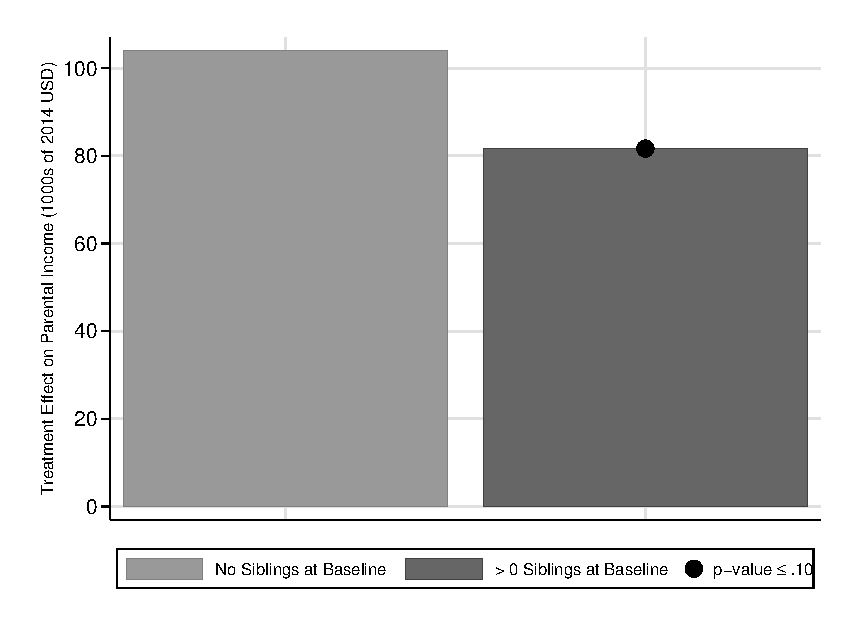
\includegraphics[width=\textwidth]{output/abccare_pinc_npv_pooled.eps}
\end{subfigure}%
\begin{subfigure}[h]{0.5\textwidth}
		\centering
		\caption{Siblings Younger than 5 vs. Siblings 5 or Older}
		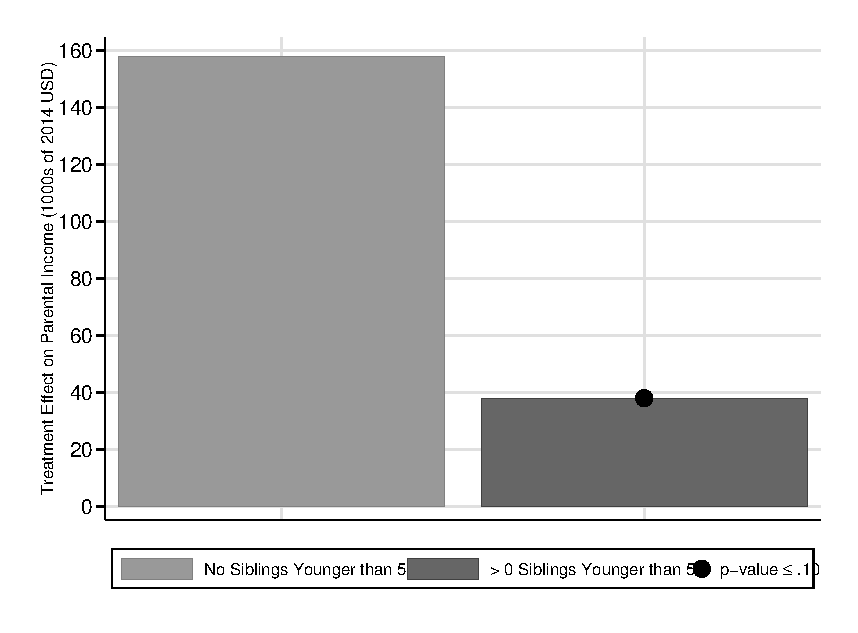
\includegraphics[width=\textwidth]{output/abccare_pinc_npv_sibs5_pooled.eps}
\end{subfigure}
\footnotesize \justify
Note: Panel (a) displays the net-present value (treatment less control) of parental labor income of parents of children with and without siblings at baseline. Panel (b) displays the average parental labor income of parents of children with young siblings (younger than 5 years old) and children with older siblings (5 years old or older) at baseline. Panel (b) drops children without siblings at baseline. Parental income is in 2014 USD discounted to child's participant age 0 using a 3\% rate.  We use the measure of parental labor income in Section~\ref{section:pincome}.
\end{figure}

\noindent \textbf{Summary: Forecasts of Parental Labor Income}\\
\noindent Any forecast of parental labor income starts at the last observation of parental labor income, which varies by individual due to sample attrition. We assume that parental labor income is equal to maternal income (only 27\% of mothers in ABC/CARE report living in a two-parent home).
\begin{enumerate}
\item \textbf{Mincer Model}
\begin{enumerate}
\item \textbf{Auxiliary Sample Used to Forecast:} PSID.
\item \textbf{Initial Restrictions Placed on the Auxiliary Sample:} Black; female; unmarried; education and number of children at ages 5 in the ranges of ABC/CARE participants. Labor income at each age is below the 75th percentile.
\item \textbf{Variables Used to Construct Synthetic Control and Treatment Groups:} we pool PSID/NLSY79 restricted samples.
\item \textbf{Variables Used to Forecast:} education, second order polynomial in experience, birth year, number of children.
\item \textbf{Assumed Retirement:} after 40 years of labor force participation.
\end{enumerate}
\item \textbf{Life-cycle Forecast}
\begin{enumerate}
\item \textbf{Auxiliary Sample Used to Forecast:} PSID and NLSY79.
\item \textbf{Initial Restrictions Placed on the Auxilliary Sample:} Black; female; labor income at each age is below the 90th percentile.
\item \textbf{Variables Used to Construct Synthetic Control and Treatment Groups:} we pool the PSID restricted sample, and do not construct synthetic experimental groups due to lack of data on the treatment effect predictors.
\item \textbf{Variables Used to Forecast:} lagged labor income.
\item \textbf{Assumed Retirement:} 67 years old.
\end{enumerate}
\end{enumerate}

\subsection{Internal Rate of Return}
\label{app:method_irr}

\noindent To estimate the internal rate of return, we solve for $\rho$ in the following equation:
\begin{align}
\sum_{a=0}^A \frac{ \mathbb{E} (B_a - C_a)}{(1+\rho)^a} = 0,
\end{align}
where we let $A = 79$, define $B_a$ and $C_a$ to be the (discounted) total benefits and costs of the program at age $a$, and define $\mathbb{E}(.)$ to be the sample mean.\footnote{This is an abuse of notation given that $B_a$ and $C_a$ are not discounted in Appendix~\ref{app:method_irr}.} That is, we estimate the internal rate of return for the \textit{average subject} of ABC/CARE. \\

\noindent All outcomes of the parents and subjects affected by the program are treated as benefits. For this to make sense, we reverse the sign of the monetized effect of the program on specific outcomes. Costs of ABC/CARE consist only of the initial program costs from ages 0 to 5. Table \ref{table:bc_comp} provides a full list of the benefits and costs of ABC. \\

\noindent We take the sum of the treatment effects on each component of the benefits to be the total benefit, $B_a$, of the ABC/CARE program. This includes parental labor income, subject labor income, and QALYs (quality-adjusted life years). Treatment effects on costs borne by the subject or society have their signs reversed and are included as benefits. We do this for subject public-transfer income, education costs, crime costs, control substitution costs, and health costs. To account for deadweight loss, we impose a marginal welfare cost of 50\% by multiplying public costs by a factor of $0.5$ when they are a direct transfer from the government to the individuals.\footnote{There is no clear consensus on the marginal welfare cost of tax revenue. However, most researchers estimate the welfare cost per tax dollar to be between \$0.30 and \$0.50. See \citet{Feldstein_1999_REStat}, \citet{Heckman_Smith_1998_evaluating}, and \citet{Browning_1987_AER}.} When the public costs are not a direct transfer from the government to the individuals, we multiply them by a factor of $1.5$.

\noindent The principle for multiplying the public costs is the following. We evaluate the social benefits of ABC/CARE and do not place a value on who receives the money. The only social cost from a direct transfer is the dead-weight loss that it generates: $50\%$ of its total value. We do not consider education and criminal costs to be a direct transfer. Thus, we multiply them by a factor of $1.5$: the value of their cost plus $50\%$ of the value of their cost (the dead-weight loss implied in raising the public revenue to fund them). Table \ref{table:bc_comp} lists the factor we use to multiply each cost to account for its implied dead-weight loss.

\noindent Having constructed our cash flow, $\mathbb{E} (B_a - C_a)$, solving for $\rho$ reduces to an algebraic exercise. The expected life-cycle profile of net benefits need to satisfy a ``single crossing property'' in order to obtain a unique solution for the internal rate of return.\footnote{See \citet{Arrow-Levhari_1969_EJ} for a formal discussion, although the discussion on multiplicity, sign, and real or complex nature of the roots of a polynomial traces back to Descartes' Rule.} The single crossing property holds when the benefits do not go from positive to negative across the life cycle. When the single crossing property is not satisfied, the internal rate of return is not a valid summary for the efficiency of an investment. To calculate the internal rate of return, we estimate the treatment effect on each component of the benefits and costs at age $a$ for the pooled, male, and female samples. We do this for 100 bootstrap resamples of the original ABC/CARE data. In the case of health costs and subject income, for which we employ auxiliary datasets to estimate the treatment effects, we also obtain 100 bootstrap estimates from the auxiliary data for every ABC/CARE bootstrap resample, resulting in a total of 100,000 estimates. By reusing each bootstrap estimate of the treatment effect on outcomes that do not require any auxiliary data set 100 times, we obtain a total of 100,000 estimates of the cash flow. We estimate the internal rate of return on each of those cash flows, and discard those for which we find a negative internal rate of return. The remaining estimates form our empirical bootstrap distribution of the internal rate of return for the pooled, male, and female samples. We take the mean of the distributions to be the point estimates, and we take the sample standard deviations to be the standard errors. To construct the 80\% confidence intervals, we take the 10\textsuperscript{th} and 90\textsuperscript{th} percentiles of each bootstrap distribution.

\noindent Figure~\ref{figure:irrdist} reports the distributions of the internal rates of return, by gender and for each of the three parameters that we consider (treatment vs. next best, treatment staying at home, treatment vs. alternative preschool). For some parameters and genders, we discard a high percentage of the internal rate of return of the outcomes. We next discuss how we calculate the benefit/cost ratios, noting that this statistic is not subject the same caveat as the internal rate of return: we can summarize the efficiency of the investment even in the absence of the single-crossing property.

\newgeometry{top=.6in, bottom=.8in, left=.6in, right=.6in}
\begin{sidewaysfigure}[!htbp]
\centering
\caption{Internal Rate of Return, by Gender and by Parameter}\label{figure:irrdist}
\begin{subfigure}[h]{0.25\textwidth}
		\centering
		\caption{Treatment vs. Next Best, Pooled}
		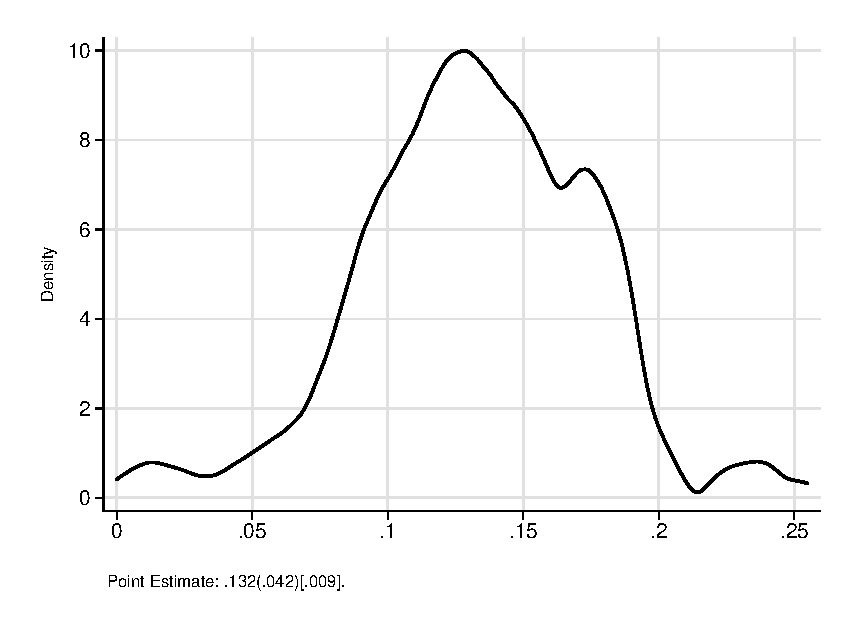
\includegraphics[width=\textwidth]{output/irr_2_sexp.eps}
\end{subfigure}%
\begin{subfigure}[h]{0.25\textwidth}
	\centering
	\caption{Treatment vs. Next Best,\\ Females}
		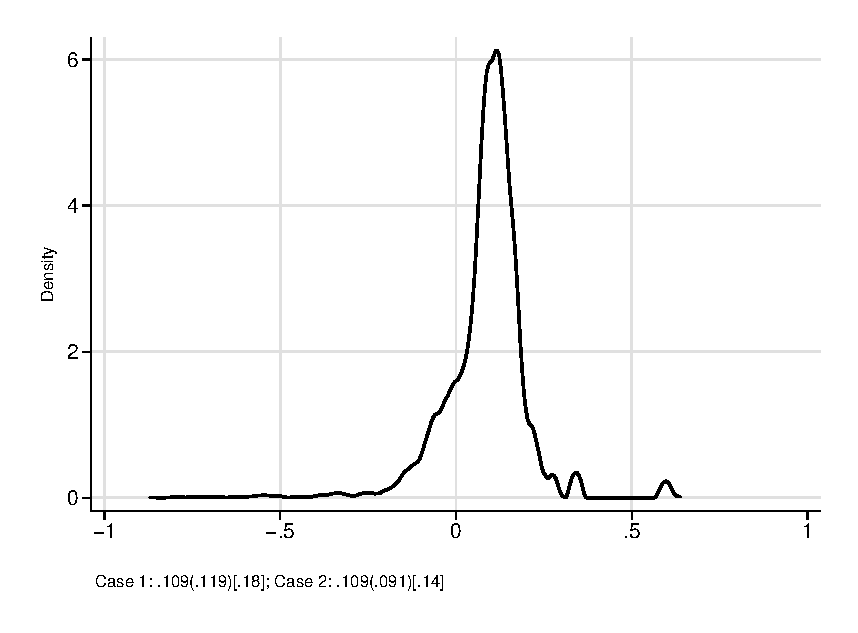
\includegraphics[width=\textwidth]{output/irr_2_sexf.eps}
\end{subfigure}%
\begin{subfigure}[h]{0.25\textwidth}
		\centering
		\caption{Treatment vs. Next Best, Males}
		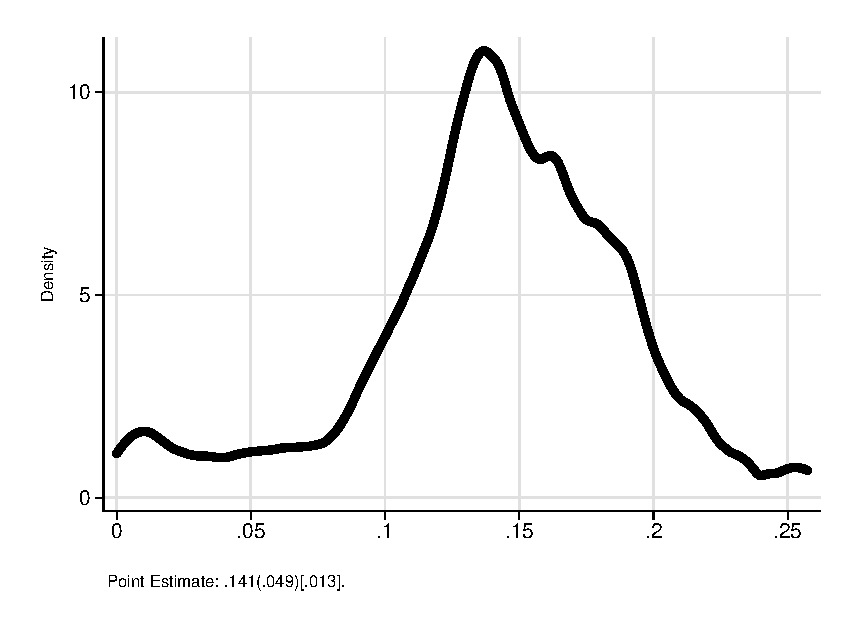
\includegraphics[width=\textwidth]{output/irr_2_sexm.eps}
\end{subfigure}
\begin{subfigure}[h]{0.25\textwidth}
	\centering
	\caption{Treatment vs. Staying at Home, Pooled}
		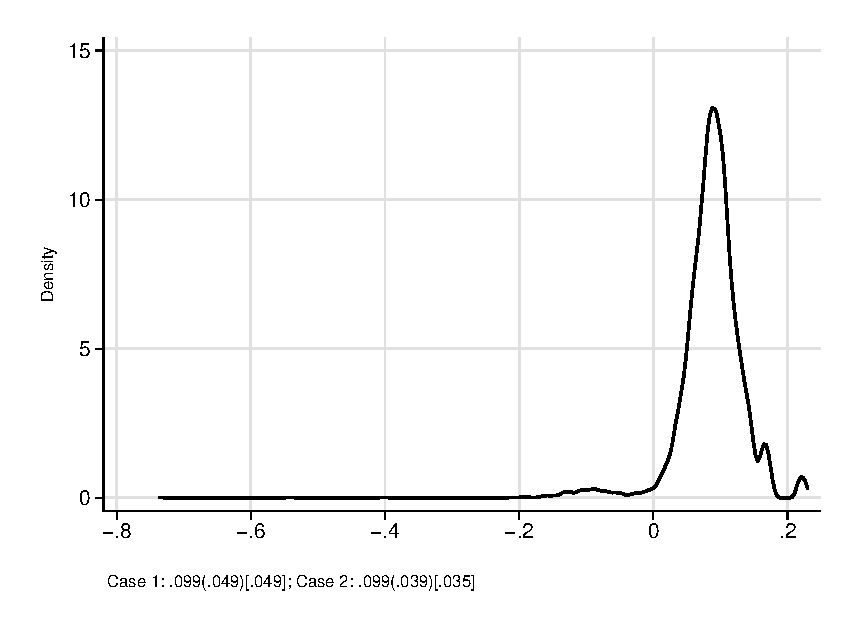
\includegraphics[width=\textwidth]{output/irr_5_sexp.eps}
\end{subfigure}%
\begin{subfigure}[h]{0.25\textwidth}
	\centering
	\caption{Treatment vs. Staying at Home, Females}
		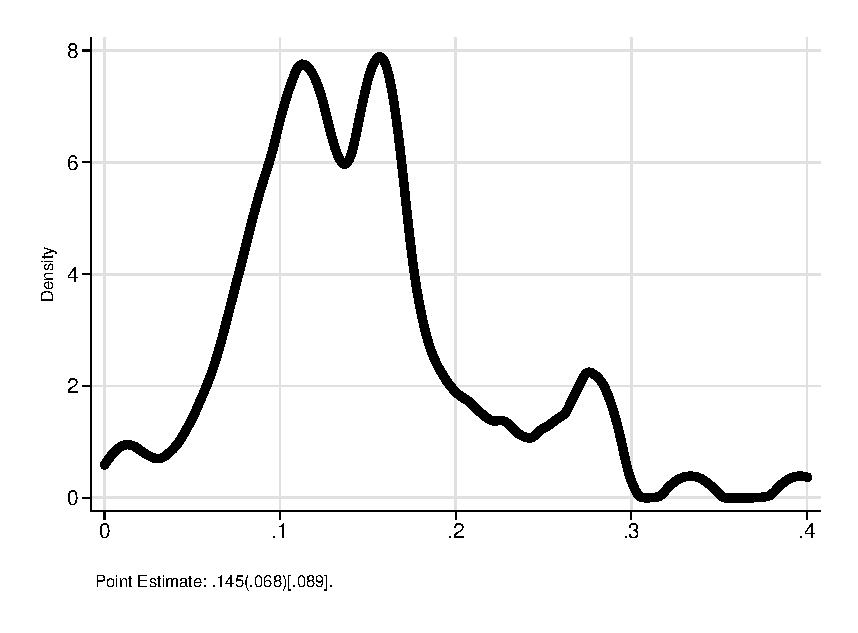
\includegraphics[width=\textwidth]{output/irr_5_sexf.eps}
\end{subfigure}%
\begin{subfigure}[h]{0.25\textwidth}
	\centering
	\caption{Treatment vs. Staying at Home, Males}
		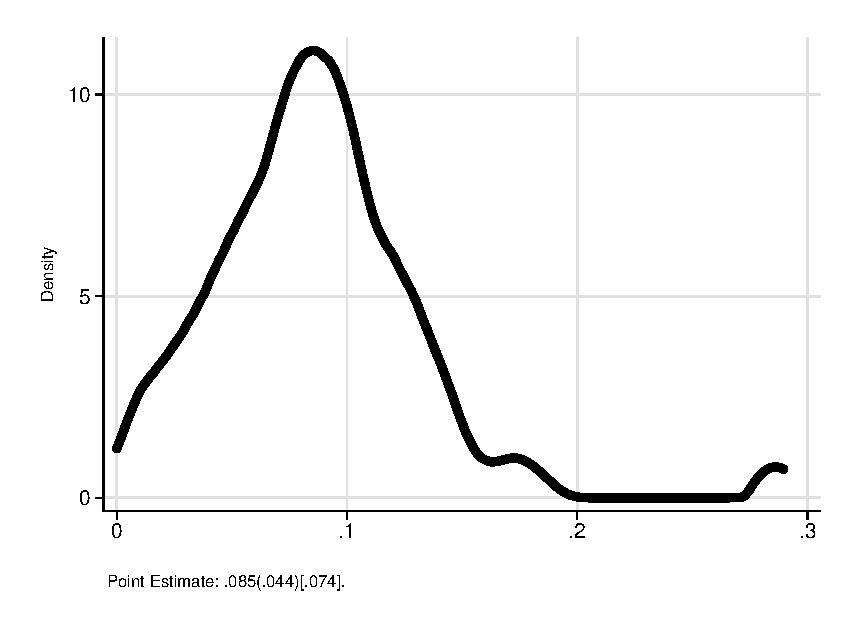
\includegraphics[width=\textwidth]{output/irr_5_sexm.eps}
\end{subfigure}
\begin{subfigure}[h]{0.25\textwidth}
	\centering
	\caption{Treatment vs. Alternative Preschool, Pooled}
		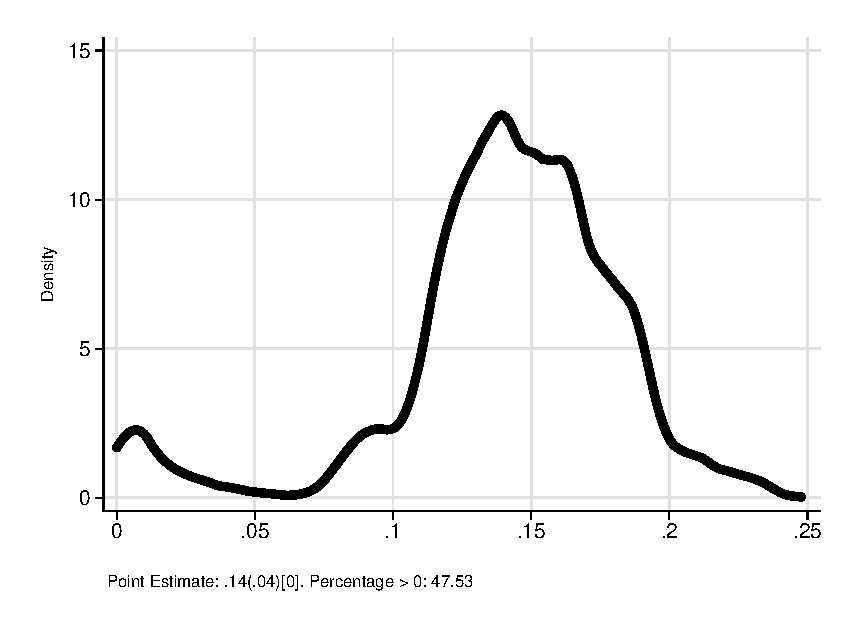
\includegraphics[width=\textwidth]{output/irr_8_sexp.eps}
\end{subfigure}%
\begin{subfigure}[h]{0.25\textwidth}
	\centering
	\caption{Treatment vs. Alternative Preschool, Females}
		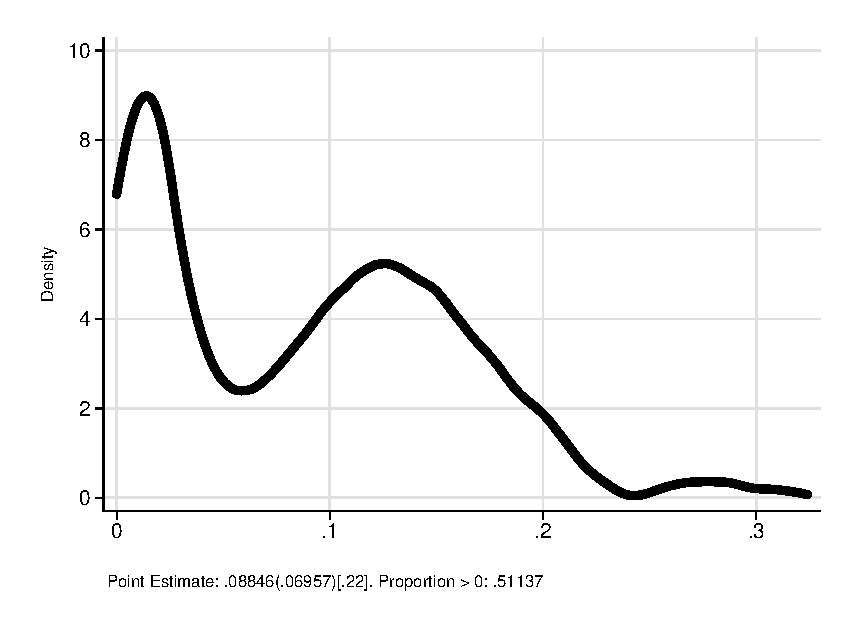
\includegraphics[width=\textwidth]{output/irr_8_sexf.eps}
\end{subfigure}%
\begin{subfigure}[h]{0.25\textwidth}
	\centering
	\caption{Treatment vs. Alternative Preschool, Males}
		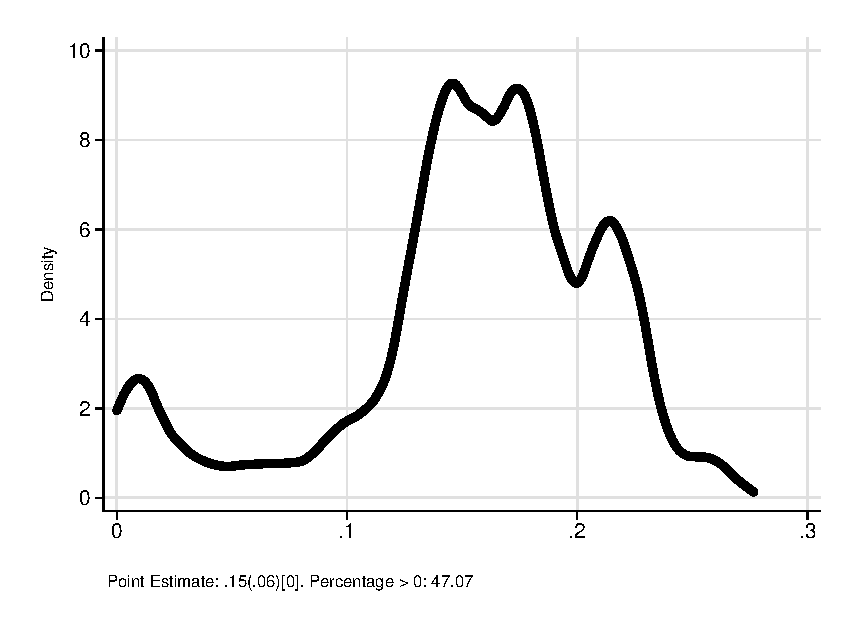
\includegraphics[width=\textwidth]{output/irr_8_sexm.eps}
\end{subfigure}
\footnotesize \justify
Note: Panel (a) displays the empirical bootstrap distribution for the estimate of the treatment vs. next parameter in the pooled sample. The remaining panels show an analogous distribution when varying the parameter and the gender. See Appendix~\ref{appendix:cbaresultscont} for the definition of the parameters. We discard negative internal rates of returns. Each panel displays the point estimate with the standard error in parentheses, the $p$-value in brackets, and the percentage of positive internal rates of return out of the initial set of bootstrap resamples.
\end{sidewaysfigure}
\restoregeometry
\doublespacing




% We let $T = 79$. In Appendix \ref{app:method_identify}
% we explain how we can estimate the summand of the numerator at every period $t$, which
% can be expressed as $\mathbf{E}(B_t) -  \mathbf{E}(C_t)$. Thus, solving for $\rho$
% reduces to an algebraic exercise.



% To construct our cash flow, we subtract the costs from benefits to create a single stream.
% We define `cost' to include only the program costs of ABC, and define
% `benefits' to include all treatment effects of the program. This includes
% the treatment effects on parent income, subject labor income, and QALY
% (quality adjusted life years).\footnote{QALYs are measured on a scale of 0 to 1, with 1 being a
% year of perfect health. We follow \textbf{[CITATION]} and value a QALY of 1 to be
% \$150,000, and a QALY of 0 to be \$0. The dollar value of that year relates linearly to the QALY.}
% Treatment effects on costs borne by the subject or society have their signs
% reversed and are included as benefits. We do this for subject transfer income,
% education costs, jail costs, justice system costs, victimization costs,
% control contamination costs, and medical costs. To account for deadweight loss, we
% impose a marginal welfare cost of 50\% by multiplying public costs by a factor of
% $1.5$.\footnote{There is no clear consensus on the marginal welfare cost of tax revenue. However,
% most researchers estimate the welfare cost per tax dollar is between \$0.30--0.50. See
% \citet{feldstein1999tax, heckman1998evaluating, browning1987marginal}.} This
% includes education cost up until age 17, jail costs, justice system costs, Medicare costs,
% and Medicaid costs. For the same reason, we multiply transfer income by a factor of 0.5.

% For each period $t \in \{1, 2, \dots, 79\}$, we sum our estimates of the benefits, and
% subtract our estimates of the costs from that sum. This provides us an estimate of
% $\mathbf{E}(B_t) -  \mathbf{E}(C_t) = \mathbf{E} (B_t - C_t)$. We then solve for
% $\rho$ using numerical analysis.

% In your methodlogy you describe costs and benefits differnetly....
% To construct our cash flow, we sum the costs and benefits from the program into a single stream.
% We define `cost' to include only the cost of implementing ABC. On the other hand,
% we broadly define `benefits' to include all treatment effects of the program. This includes
% the treatment effects on parent income, subject labor income, and QALY
% (quality adjusted life years).\footnote{QALYs are measured on a scale of 0 to 1, with 1 being a
% year of perfect health. We follow \textbf{[CITATION]} and value a QALY of 1 to be
% \$150,000, and a QALY of 0 to be \$0. The dollar value of that year relates linearly to the QALY.}
% Treatment effects on outcomes generally considered to be costs have their signs reversed in
% order to convert them into benefits. We do this for subject transfer income,
% education costs, jail costs, justice system costs, victimization costs,
% control contamination costs, and medical costs. To account for deadweight loss, we
% impose a marginal welfare cost of 50\% by multiplying public costs by a factor of
% $1.5$.\footnote{There is no clear consensus on the marginal welfare cost of tax revenue. However,
% most researchers estimate the welfare cost per tax dollar is between \$0.30--0.50. See
% \citet{feldstein1999tax, heckman1998evaluating, browning1987marginal}.} This
% includes education cost up until age 17, jail costs, justice system costs, Medicare costs,
% and Medicaid costs. For the same reason, we multiply transfer income by a factor of 0.5.


\subsection{Computing the Benefit/Cost Ratio}\label{app:method_cbratio}

\noindent The benefit/cost ratio is
\begin{align}
\mathbb{E} \left( \frac{ \sum_{a=0}^A B_a}{\sum_{a=0}^A C_a} \right),
\end{align}

\noindent where we let $A = 79$, define $B_a$ and $C_a$ to be the benefits and costs of the
program at age $a$, and define $\mathbb{E}(.)$ to be the sample mean. See Table \ref{table:bc_comp} for a detailed list of the components
to the benefits and costs of ABC/CARE . We take the sum of the treatment effects on each component
of the benefits to be the total benefits of the ABC/CARE programs. \\

\noindent To account for deadweight loss, we assume a marginal welfare cost of 50\% by multiplying
public costs components by a factor of $1.5$. For the same reason, we multiply public-transfer
income by a factor of 0.5. We discount each component of the benefits and costs
by 3\% every year to obtain their net present value at birth. We then sum up the discounted
components of the benefits and find the ratio with the discounted costs. \\

\noindent We estimate the treatment effect for each component of the benefits and costs at age $a$ for the pooled, male, and female samples. We do this for 100 bootstrap resamples of the original ABC/CARE data. In the case of health and subject income, for which we employ auxiliary datasets to estimate the treatment effects, we also obtain 100 bootstrap estimates from the auxiliary data for every ABC/CARE bootstrap resample, resulting in a total of 100,000 estimates. By reusing each bootstrap estimate of the treatment effect on outcomes that do not require any auxiliary data set 100 times, we obtain a total of 100,000 estimates of the costs stream and benefits stream. We estimate the benefit/cost ratio for each of those streams. This is how we form our empirical bootstrap distribution of the benefit/cost ratio for the pooled, male, and female samples. We take the mean of the distributions to be the point estimates, and we take the standard deviations to be the standard errors. To construct the 80\% confidence intervals, we take the 10\textsuperscript{th} and 90\textsuperscript{th} percentiles of each bootstrap distribution. Figure~\ref{figure:ratiodist} presents the empirical distribution of the empirical bootstrap distribution, per parameter of interest and gender.

\begin{table}[H]
\begin{threeparttable}
\caption{Components of Benefits and Costs}
\label{table:bc_comp}
\centering
\begin{tabular}{l c c}
\toprule			
Variable & Sign Reversed	& Welfare Cost \\
	&		& Factor \\
\midrule
\textbf{Benefits} 	\\			
\quad Parent Income			& \\
\quad Subject QALY			& \\
\quad Subject Labor Income	& \\
\quad Subject Public-transfer Income	& $\checkmark$	& 0.5 \\
\quad Medicare Costs			& $\checkmark$	& 1.5 \\
\quad Medicaid Costs			& $\checkmark$	& 1.5 \\
\quad Out-of-pocket Medical Costs	& $\checkmark$ \\
\quad Miscellaneous Medical Costs	& $\checkmark$ \\
\quad Disability Insurance Claim	& $\checkmark$	&	1.5 \\
\quad Social Security Claim	& $\checkmark$	&	1.5 \\
\quad Supplemental Security Claim	& $\checkmark$	&	1.5 \\
\quad Control Substitution Costs	& $\checkmark$	& \\
\quad Education Costs			& $\checkmark$	& 1.5* \\
\quad Justice System Costs	& $\checkmark$	& 1.5 \\
\quad Prison Costs			& $\checkmark$	& 1.5 \\
\quad Victimization Costs		& $\checkmark$	& \\
\textbf{Costs} 	\\			
\quad Program Costs			& \\
\bottomrule			
\end{tabular}
\begin{tablenotes}
\footnotesize
\item Note: The table lists the components of the costs and benefits of ABC/CARE.
In order for some components to be categorized as benefits, we reversed the sign
of the treatment effect. Only education costs up until age 18 are multiplied by 1.5 to account for welfare costs. This factor is drawn from \citet{Heckman_Moon_etal_2010_RateofReturn}.
\end{tablenotes}
\end{threeparttable}
\end{table}

\newgeometry{top=.6in, bottom=.8in, left=.6in, right=.6in}
\begin{sidewaysfigure}[!htbp]
\centering
\caption{Benefit/Cost Ratios, by Gender and by Parameter}\label{figure:ratiodist}
\begin{subfigure}[h]{0.25\textwidth}
		\centering
		\caption{Treatment vs. Next Best, Pooled}
		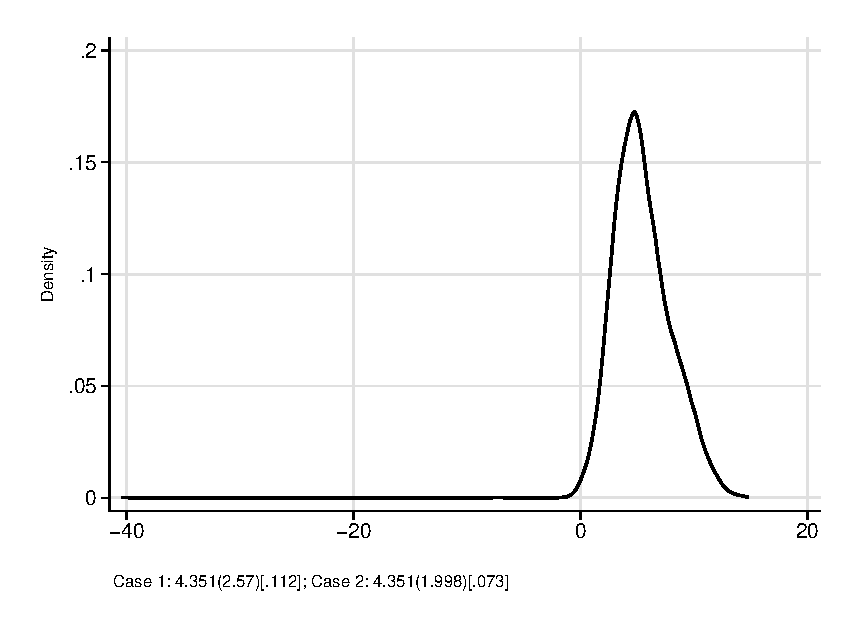
\includegraphics[width=\textwidth]{output/ratios_2_sexp.eps}
\end{subfigure}%
\begin{subfigure}[h]{0.25\textwidth}
	\centering
	\caption{Treatment vs. Next Best,\\ Females}
		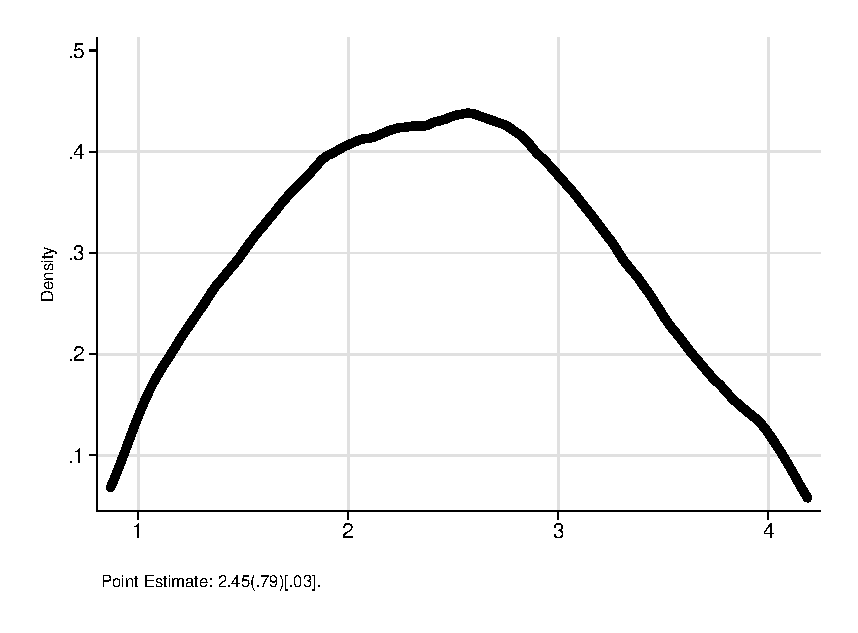
\includegraphics[width=\textwidth]{output/ratios_2_sexf.eps}
\end{subfigure}%
\begin{subfigure}[h]{0.25\textwidth}
		\centering
		\caption{Treatment vs. Next Best, Males}
		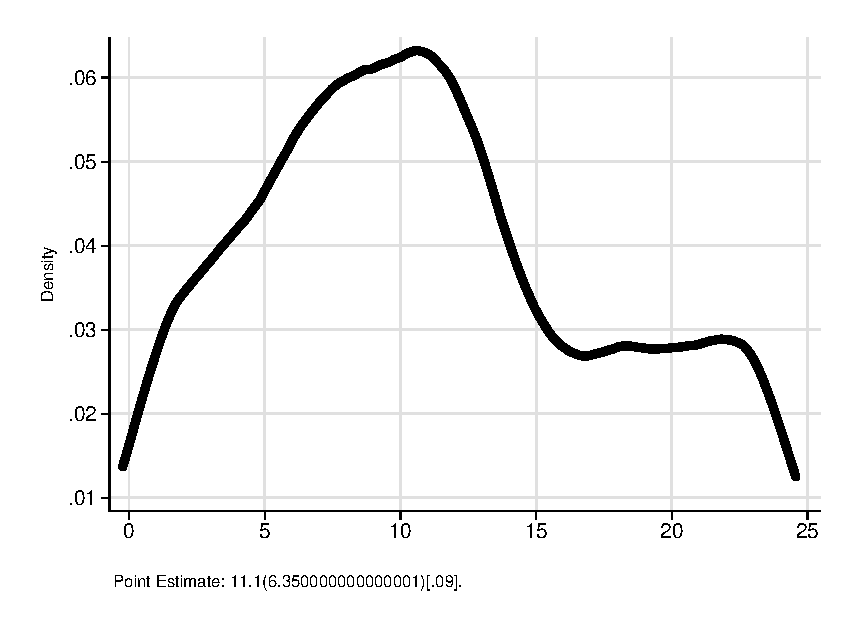
\includegraphics[width=\textwidth]{output/ratios_2_sexm.eps}
\end{subfigure}
\begin{subfigure}[h]{0.25\textwidth}
	\centering
	\caption{Treatment vs. Staying at Home, Pooled}
		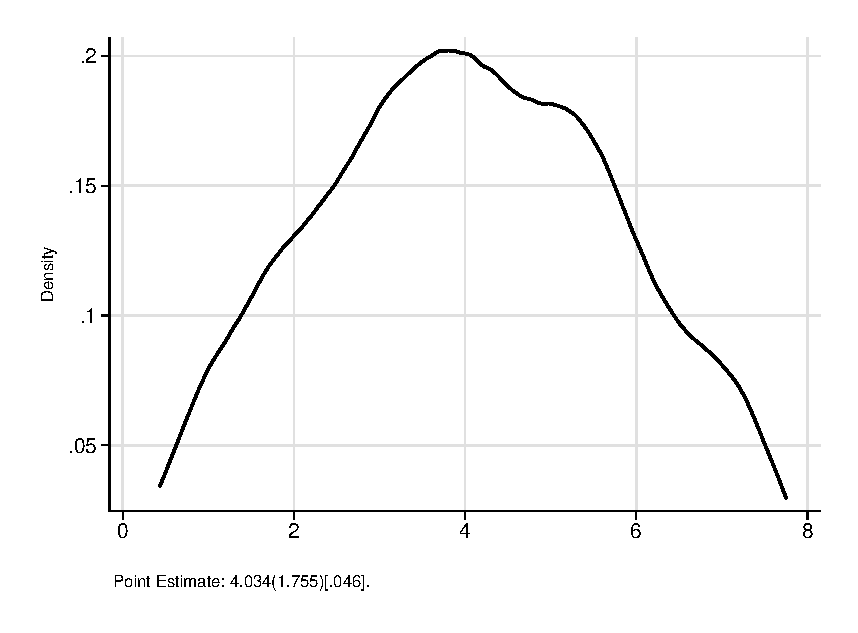
\includegraphics[width=\textwidth]{output/ratios_5_sexp.eps}
\end{subfigure}%
\begin{subfigure}[h]{0.25\textwidth}
	\centering
	\caption{Treatment vs. Staying at Home, Females}
		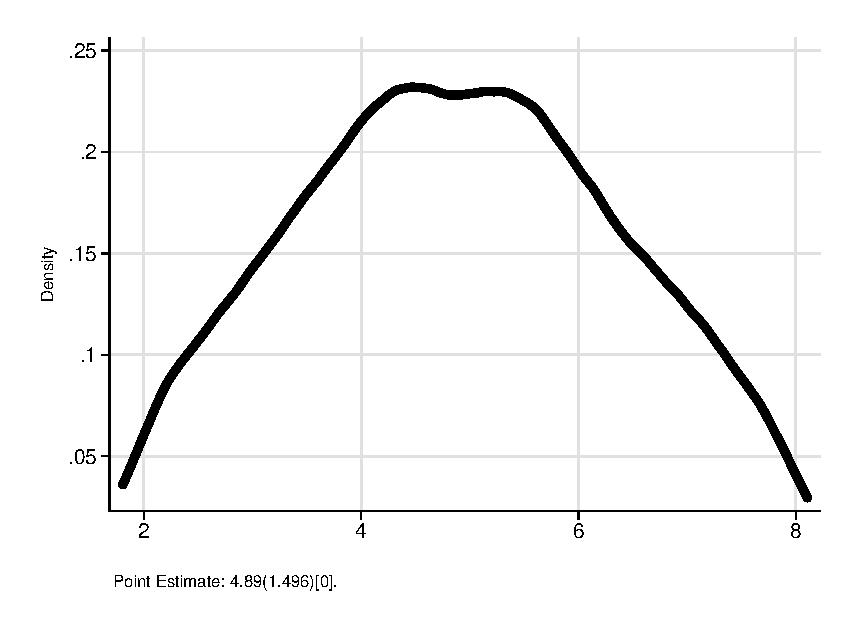
\includegraphics[width=\textwidth]{output/ratios_5_sexf.eps}
\end{subfigure}%
\begin{subfigure}[h]{0.25\textwidth}
	\centering
	\caption{Treatment vs. Staying at Home, Males}
		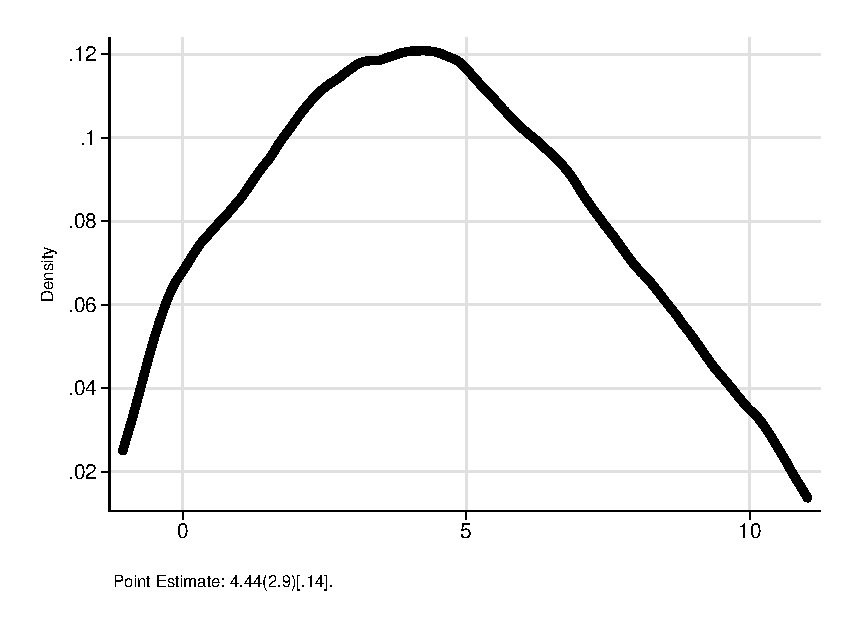
\includegraphics[width=\textwidth]{output/ratios_5_sexm.eps}
\end{subfigure}
\begin{subfigure}[h]{0.25\textwidth}
	\centering
	\caption{Treatment vs. Alternative Preschool, Pooled}
		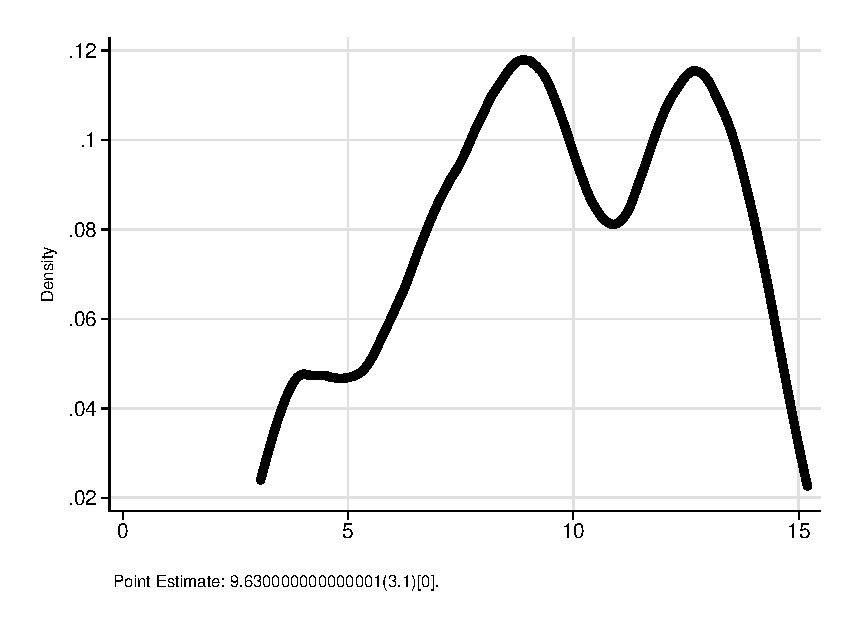
\includegraphics[width=\textwidth]{output/ratios_8_sexp.eps}
\end{subfigure}%
\begin{subfigure}[h]{0.25\textwidth}
	\centering
	\caption{Treatment vs. Alternative Preschool, Females}
		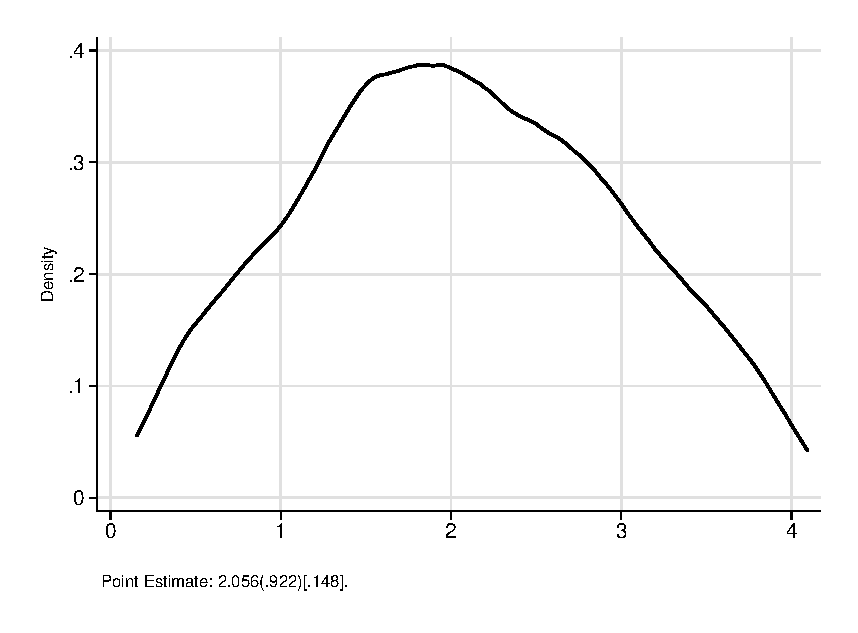
\includegraphics[width=\textwidth]{output/ratios_8_sexf.eps}
\end{subfigure}%
\begin{subfigure}[h]{0.25\textwidth}
	\centering
	\caption{Treatment vs. Alternative Preschool, Males}
		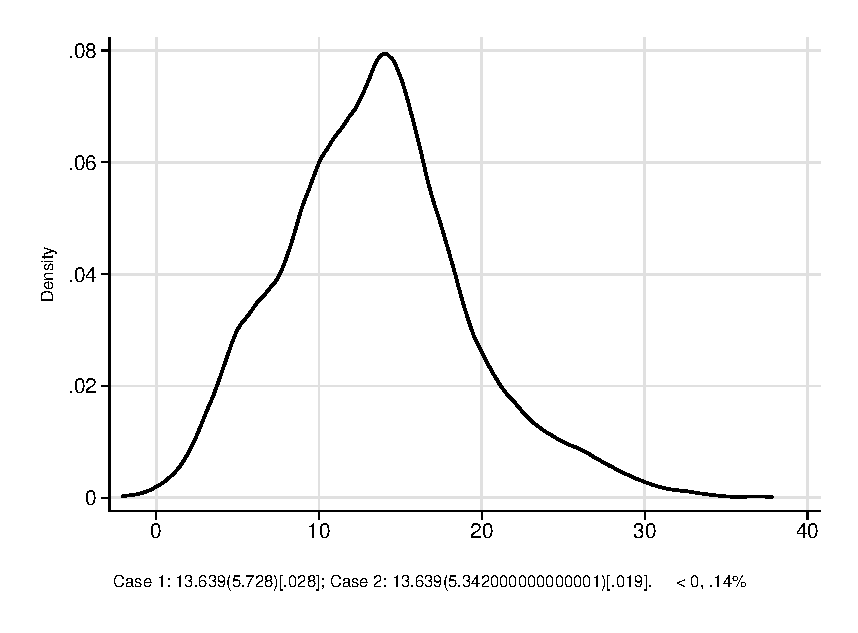
\includegraphics[width=\textwidth]{output/ratios_8_sexm.eps}
\end{subfigure}
\footnotesize \justify
Note: Panel (a) displays the empirical bootstrap distribution for the estimate of the treatment vs. next parameter in the pooled sample. The remaining panels show an analogous distribution varying the parameter and the gender. See Appendix~\ref{appendix:cbaresultscont} for the definition of the parameters. Each panel displays the point estimate with the standard error in parentheses and the $p$-value in brackets.
\end{sidewaysfigure}
\restoregeometry
\doublespacing

\subsection{Exploring the Impact of Other Forecasting Models} \label{appendix:predsensitivity}

Our analysis is based on a causal model for treatment ($d=1$) and control ($d=0$) outcomes for measure $j$ at age $a$ in sample $k \in \{e,n\}$. We explore a range of standard panel data specifications for the error terms:

\begin{eqnarray}
\varepsilon^d_{k,j,a} &=& f^d + \omega^d_{k,j,a} \nonumber \\
\omega^d_{k,j,a}      &=& \rho \omega^d_{k,j,a-1} + U^d_{k,j,a},
\end{eqnarray}

\noindent where $U^d_{k,j,a} \independent \bm{X}^d_{k,a}$.

Here, we present different structures for $\phi_{k,j,a}^d \left( \cdot, \cdot \right)$ and $\varepsilon_{k,j,a}^d$ and investigate the robustness of our estimates to different assumptions about the structure of both these elements. We do this exercise for labor income.\footnote{In Appendix~\ref{appendix:gmm}, we describe the precise steps that we follow to construct out-of-sample forecasts based on these different structures and frame our estimation strategy in a GMM framework \citep{Hansen_1982_Econometrica}.}

Note that Assumption~\ref{ass:summary} (Invariance) implies that $\phi_{k,j,a}^d \left (\cdot, \cdot \right) = \phi_{k,j,a}  \left (\cdot, \cdot \right) = \phi_{j,a}  \left (\cdot, \cdot \right)$. That is, invariance holds across the treatment and the control groups and invariance holds across the experimental and the auxiliary samples. It is important to note that invariance across the treatment and the control groups implies that the variables $\bm{X}_{k,a}^d$ summarize the effect of the treatment on the outcome. Given this and Assumption~\ref{ass:exog} (Exogeneity), the distribution of $\varepsilon_{k,j,a}^d$ is the same across the treatment and the control groups. We then drop the superscript in $\varepsilon_{k,j,a}^d$.

In Appendix~\ref{app:containsupport}, we also document that the support of $Y_{n,j,a}^d, \bm{X}_{n,a}^d, \bm{B}_{n}$ covers the support of $Y_{e,j,a}^d, \bm{X}_{e,a}, \bm{B}_{e}$ for $d \in \{0, 1\}$. This allows us to drop the $d$ superscript in $Y_{n,j,a}^d, \bm{X}_{n,a}^d$ given that we estimate an invariant model.

We use linear specifications of $\phi_{j,a}$. We explore different alternatives. The system of interest is:

\begin{eqnarray}
Y_{k,j,a}                   &=& \lambda_{0} + \lambda_{1} Y_{k,j,a-1} + \lambda_{2}  \bm{X}_{k,a} + \varepsilon_{k,j,a} \nonumber \\
\varepsilon_{k,j,a} &=& \underbrace{f}_{\text{Fixed Effect}} + \underbrace{\omega_{k,j,a}}_{\text{Potentially Serially Correlated Component}} \nonumber \\
\omega_{k,j,a}      &=& \rho \omega_{k,j,a-1} + \underbrace{U_{k,j,a}}_{\text{Independent Innovation}},
\end{eqnarray}

\noindent where $U_{k,j,a} \independent \bm{X}_{k,a}$.

Table~\ref{table:predsens} summarizes the results from our exploration through two statistics: (i) the predicted net present value of labor income under different assumptions; and (ii) the overall benefit/cost ratio when the forecasts are done based on the different proposed alternatives. Estimates from the model that we use in our baseline estimations are not sensitive to the departures from serial independence that we analyze here.

In the auxiliary samples, we observe outcomes $Y_{n,j,a}$ for $a \in [a^*, \ldots, A]$. In the experimental sample, we observe the outcome $Y_{e,j,a}$ for at most two ages, depending on the outcome. We initially assume that we observe the outcome at one age ($a = a^*$). We later relax this assumption. We thus use the information in the auxiliary sample at  $a \in [a^*, \ldots, A]$ to form extrapolations for the experimental sample, where we do not observe the outcome of interest during this age interval. We produce out-of-sample forecasts and calculate the net present value of labor income under different specifications that have different assumptions. Table~\ref{table:predsens} summarizes the five specifications that we implement.

\subsubsection{Specification 1: Lagged Component ($\lambda_{1} \neq 0$); No Serial Correlation ($\rho = 0$); and No Fixed Effect ($f = 0$)} \label{app:spec1}

Our baseline estimations are constructed using this framework for labor and transfer income, crime, and health. The realized values and forecasts are close, as displayed in Figure~\ref{fig:labor-income-profiles}, to the baseline specification. We test and fail to reject the nulls of invariance across the treatment and the control groups, invariance across the experimental and auxiliary samples, and exogeneity in both the experimental and the auxiliary samples.  The tests are conducted at $a = a^*$.

\subsubsection{Specification 2: No Lagged Component ($\lambda_{1} = 0$); Serial Correlation ($\rho \neq 0$); and No Fixed Effect ($f = 0$)} \label{app:spec2}

Given that $Y_{k,j,a-1}$ is not one of the elements in $\bm{X}_{k,a}$, it is plausible that Assumption~\ref{ass:exog} (Exogeneity) holds even when we do not restrict $\rho$. In this case, it is straightforward to account for serial correlation.\footnote{Serial correlation can be accounted for in a general way using the Newey-West approach \citep{Newey-West_1986_Simple-Pos}.}

The predictions reported in the baseline estimates are extremely similar to the ones generated in this case. That is, the lag does not help in generating predictions as much as one might think it would. This is more evidence in favor of $\bm{X}_{k,a}$ summarizing the treatment effects.

\subsubsection{Specification 3: Lagged Component ($\lambda_{1} \neq 0$); Serial Correlation ($\rho \neq 0$); and No Fixed Effect ($f = 0$)} \label{section:laggedserial}

These estimates indicate that serial correlation is present in the data. From ages 21 to 30, we estimate the model in the CNLSY. The estimate for $\rho$ is $0.7465$. From ages 30 to 67 (assumed retirement) we estimate the model on the NLSY79/PSID. The estimate for $\rho$ is $0.5426$. When we restrict the sample to people who earn \$30,000 (2014) at each of these ages, the analogous estimates of $\rho$ are $0.7370$ and $0.5316$. These estimates are statistically significant at the 1\% level.

We can $\rho$-transform the system of interest to obtain consistent estimates. Drop the $j$ index for simplicity and write:

\begin{equation}
Y_{k,a} = \lambda_{0} \left( 1 - \rho \right) + \left( \lambda_{1} + \rho \right) Y_{k,a-1} - \lambda_{1} \rho Y_{k,a-2} + \lambda_{2} \left( \bm{X}_{k,a} - \rho \bm{X}_{k,a-1}  \right) + U_{k,a}. \label{eq:rhotransform}
\end{equation}

OLS produces consistent estimates of the coefficients in Equation~\eqref{eq:rhotransform}. This enables us to construct forecasts, as explained in Appendix~\ref{appendix:gmm}. This model generates forecasts close to the baseline estimates.

\subsubsection{Specification 4: Permanent-Transitory Decomposition of Unobserved Components ($\lambda_{1} \neq 0$; $\rho = 0$; $f \neq 0$)} \label{app:permtrans}

This framework allows for serial dependence due to the lagged dependent variable but does not allow for serial correlation in $\eta_{a}$. We explain our estimation strategy for this specification in Appendix~\ref{appendix:gmm}. Estimates from it are very similar to those from the other procedures.

\subsubsection{Specification 5: Non-Parametric Predictions}

An alternative to any of these scenarios is to make forecasts using a non-parametric matching algorithm. Specifically, (i) for each individual $i$ in the experimental sample, $e$, find individual(s) $l(i)$ in the non-experimental sample, $n$, using Algorithm~\ref{alg:match} in Appendix~\ref{appendix:match}; (ii) we impute the post-$a^*$ trajectory of $Y_{k,j,a}$ of individual(s) $l(i)$ in the non-experimental sample, $n$, to individual $i$ in the experimental sample, $e$.

A sufficient condition for the validity of this procedure is Assumption~\ref{ass:exog} (Exogeneity). Without exogeneity, the joint distributions of $\bm{X}_{j,a*}, \varepsilon_{j,a^*}$ do not necessarily coincide across the experimental and the auxiliary samples. For example, in the experimental sample, individuals in the treatment group have relatively high levels of education due in part to the exogenous boost generated by randomization into treatment. In the auxiliary sample, the usual form of ability bias may be at work: individuals with relatively high levels of education might have better motivation, better parents, etc. Thus, the empirical relationships between education and labor income may differ across experimental and auxiliary samples. Exogeneity avoids this problem, but clearly only a weaker assumption is required.

\begin{sidewaystable}[H]
\resizebox{\columnwidth}{!}{%
\begin{threeparttable}
\caption{Net Present Value of Labor Income and Cost/Benefit Analysis Under Different Specifications for Labor Income Forecasts}
\label{table:predsens}
\centering
\footnotesize
\begin{tabular}{L{2cm} *7{C{1.5cm}}} \toprule
& \multicolumn{3}{c}{ \textbf{Specification 1:}} & & \multicolumn{3}{c}{ \textbf{Specification 2:}}\\
& \multicolumn{3}{c}{Lagged component in $\bm{\phi}_{j,a}$} & & \multicolumn{3}{c}{No lagged component in $\bm{\phi}_{j,a}$} \\
& \multicolumn{3}{c}{ set $\bm{\rho} = 0$} & & \multicolumn{3}{c}{Unrestricted $\bm{\rho}$} \\[10pt]

& NPV & IRR & B/C & & NPV & IRR & B/C \\

\hline \\
Pooled & 71,345 & 0.13 & 6.29 & & 154,547 & 0.26 & 12.39 \\ 
& (86,343) & (.05) & (2.11) & & (187,036) & (0.11) & (5.16) \\ \\

Males & 300,896 & 0.13 & 11.1 & & 200,509 & 0.09 & 7.62 \\ 
& (241,588) & (0.06) & (6.35) & & (160,988) & (0.04) & (3.73) \\ \\ 

Females & 59,390 & 0.10 & 2.45 & & 79,441 & 0.15 & 3.61 \\ 
& (63,060) & (0.07) & (0.79) & & (99,416) & (0.11) & (1.56) \\ \\ \\

\midrule
& \multicolumn{3}{c}{ \textbf{Specification 3:}} & & \multicolumn{3}{c}{ \textbf{Specification 4:}}\\
& \multicolumn{3}{c}{Lagged component in $\bm{\phi}_{j,a}$} & & \multicolumn{3}{c}{Lagged component in $\bm{\phi}_{j,a}$; Permanent} \\
& \multicolumn{3}{c}{Unrestricted $\bm{\rho}$} & & \multicolumn{3}{c}{Transitory unobserved components} \\[10pt]

& NPV & IRR & B/C & & NPV & IRR & B/C \\

\hline \\
Pooled & 268,179 & 0.49 & 23.64 & & 46,953 & 0.09 & 4.14 \\ 
& (211,089) & (0.12) & (5.16) & & (25,323) & (0.01) & (0.62) \\ \\

Males &456,078 & 0.2 & 16.82 & & 74,775 & 0.03 & 2.76 \\ 
& (358,534) & (0.09) & (9.42) & & (54,752) & (0.01) & (1.44)  \\ \\ 

Females & 31,303 & 0.05 & 1.29 & & 19,959 & 0.03 & 0.82 \\ 
& (168,160) & (0.19) & (2.11) & & (34,142) & (0.04) & (0.43) \\ \\ \\


\midrule
& & & \multicolumn{3}{c}{\textbf{Specification 5:}} \\
& & & \multicolumn{3}{c}{ Fully Non-Parametric} \\[10pt]
& & & NPV & IRR & B/C \\
\hline \\
& & Pooled & 62,080 & 0.10 & 4.98 \\ 
& & & (75,030) & (0.03) & (2.07) \\ \\ 
& & Males & 289,471 & 0.13 & 11.01 \\ 
& & & (232,471) & (0.06) & (5.39) \\ \\ 
& & Females & 59,163 & 0.11 & 2.69 \\ 
& & & (74,039) & (0.08) & (1.16) \\ \bottomrule
\end{tabular}
\begin{tablenotes}
\footnotesize
\item Note: This table displays the net present value of labor income in 2014 USD (treatment - control) using the five different specifications for forecasting that are explained below. Specification 1 is our baseline estimate. It also presents the calculation of the internal rate of return and the benefit/cost ratio of the program using these different net present values. Specification 1: forecast based on lagged outcome; no serial autocorrelation; and no fixed effect. Specification 2: forecast based on lagged outcome; arbitrary serial autocorrelation; and no fixed effect. Specification 3: forecast based on lagged outcome; first-order serial autocorrelation; and no fixed effects. Specification 4: forecast based on lagged outcome; no serial autocorrelation; and fixed effect.
\end{tablenotes}
\end{threeparttable}
}
\end{sidewaystable}

\subsection{Estimation Procedure and Data Combination Estimator in the GMM Framework} \label{appendix:gmm}

\noindent Our analysis is based on a causal model for treatment ($d=1$) and control ($d=0$) outcomes for measure $j$ at age $a$ in sample $k \in \{e,n\}$ where $e$ denotes membership in the experimental sample and $n$ denotes membership in the auxiliary sample:\\

\begin{equation}\label{eq:outcome}
Y^d_{k,j,a} = \phi^d_{k,j,a} (\bm{X}^d_{k,a}, \bm{B}_k) + \varepsilon^d_{k,j,a}, \quad k \in \{n,e\}, \quad j \in \mathcal{J}_a, \quad d \in \{0, 1\}.
\end{equation}

\noindent $\phi^d_{k,j,a}\left( \cdot, \cdot \right)$ is an invariant structural production relationship mapping inputs $\bm{X}^d_{k,a}, \bm{B}_k$ into output $Y^d_{k,j,a}$ (in this Appendix a scalar, for illustration purposes) holding error term $\varepsilon^d_{k,j,a}$ fixed. For simplicity, we initially assume \ref{ass:exog} (Exogeneity) holds. We relax this below.

\noindent In this section, we: (i) explain the procedure that we follow to form out-of-sample forecasts; and (ii) formulate the estimation procedure in a generalized method of moments (GMM) framework \citep{Hansen_1982_Econometrica}.

\noindent In the auxiliary sample, we observe the outcome $Y_{n,j,a}$ for $a \in [a^*, \ldots, A]$. In the experimental sample, we observe the outcome $Y_{e,j,a}$ for at most two ages, depending on the outcome. We initially assume that we observe the outcomes at one age ($a^*$). We relax this assumption below.

\noindent Before explaining our estimation procedure, note that Assumption~\ref{ass:summary} (Invariance) implies that $\phi_{k,j,a}^d \left (\cdot, \cdot \right) = \phi_{k,j,a}  \left (\cdot, \cdot \right) = \phi_{j,a}  \left (\cdot, \cdot \right)$. That is, invariance holds across the treatment and the control groups and invariance holds across the experimental and the auxiliary samples. Invariance across the treatment and the control groups implies that the variables $\bm{X}_{k,a}^d$ summarize the effect of the treatment on the outcome. Given Assumption~\ref{ass:summary} (Invariance)  and Assumption ~\ref{ass:exog} (Exogeneity), the distribution of $\varepsilon_{k,j,a}^d$ is the same across the treatment and the control groups. This allows us to drop the superscript in $\varepsilon_{k,j,a}^d$.

\noindent We test and do not reject invariance across the treatment and the control groups and invariance across the experimental and the auxiliary samples in the main paper.

\noindent In Appendix~\ref{app:containsupport}, we document that the support of $Y_{n,j,a}^d, \bm{X}_{n,a}^d, \bm{B}_{n}$ covers the support of $Y_{e,j,a}^d, \bm{X}_{e,a}, \bm{B}_{e}$ for $d \in \{0, 1\}$. So we drop the $d$ superscript in $Y_{n,j,a}^d, \bm{X}_{n,a}^d$ given that we estimate an invariant model. We write:

\begin{equation}\label{eq:routcome}
Y_{k,j,a} = \phi_{j,a} (\bm{X}_{k,a}, \bm{B}_k) + \varepsilon_{k,j,a}, \quad k \in \{n,e\}, \quad j \in \mathcal{J}_a.
\end{equation}

\noindent As we note in Appendix~\ref{appendix:predsensitivity}, we work with a linear specification of $\phi_{j,a}$ in our empirical analysis. We explain our estimation procedure and the GMM framework for a general specification of $\phi_{j,a}$.

\noindent First, we explain our estimation and forecasting procedure using \textbf{Specification 1} in Appendix~\ref{appendix:predsensitivity}. This is the specification that we follow in the main text. It is as follows.

\begin{enumerate}
\item Use the auxiliary sample ($n$) to estimate the the coefficients characterizing $\phi_{j,a} \left( \cdot , \cdot \right)$.\footnote{In practice, we use a weighted version of the auxiliary samples. The weights give relatively high importance to the individuals in the auxiliary sample whose characteristics $\bm{B}_k$ are close to the those of the individuals in the experimental sample. See Appendix~\ref{appendix:match}.}

We denote these coefficients by $\bm{\theta}_{j,a}$ and the estimate of this function as $\hat{\phi}_{j,a} \left( \cdot , \cdot \right)$. At each age, we are able to compute the residuals from this estimation procedure as follows:

\begin{equation}
Y_{n,j,a} -  \hat{\phi}_{j,a} (\bm{X}_{k,a}, \bm{B}_k) : = \hat{\varepsilon}_{n,j,a}.
\end{equation}

For outcome $j$, we form the vector of residuals $\hat{\mathcal{E}}_{n,j} : = \left[ \hat{\varepsilon}_{n,j,a^*+1}, \ldots, \hat{\varepsilon}_{n,j,A} \right]$.

\item At age $a^*+1$, we construct the forecasted outcome for the experimental sample (e) for each individual as follows:
\begin{equation}
\hat{Y}_{e,j,a^*+1} = \hat{\phi}_{j,a^*+1} \left( \bm{X}_{e,a^*+1}, \bm{B}_e \right).
\end{equation}

\noindent We are able to evaluate $\hat{\phi}_{j,a^*+1}$ at $ \bm{X}_{e,a^*+1}, \bm{B}_e $ even when $\bm{X}_{e,a^*+1}$ contains a one-period lag of $Y_{e,j,a^*+1}$ because we observe $Y_{e,j,a^*}$. This prediction does not account for estimation error. We discuss estimation error below.

\item At age $a^*+2$, we construct the forecasted outcome in the experimental sample (e) as follows:

\begin{equation}
\hat{Y}_{e,j,a^*+2} = \hat{\phi}_{j,a^*+1} \left( \bm{X}_{e,a^*+1}, \bm{B}_e \right).
\end{equation}

\noindent We are able to evaluate $\hat{\phi}_{j,a^*+2}$ at $ \bm{X}_{e,a^*+2}, \bm{B}_e $ even when $\bm{X}_{e,a^*+2}$ contains a one-period lag of $Y_{e,j,a^*+2}$ because we can forecast $Y_{e,j,a^*+1}$ from the previous step.

\item We iterate this procedure up to age $A$. For outcome $j$, we form the vector of forecasts $\hat{\mathcal{Y}}_{e,j} : = \left[ \hat{Y}_{e,j,a^*+1}, \ldots,  \hat{Y}_{e,j,A} \right]$.

\item Under Assumption~\ref{ass:summary} (Invariance), the distribution of $\hat{\mathcal{E}}_{n,j}$ is a consistent estimator of the distribution of $\hat{\mathcal{E}}_{e,j}$. We form a forecast that accounts for forecasting error as follows:

\begin{equation}
\tilde{\mathcal{Y}}_{e,j} = \hat{\mathcal{Y}}_{e,j} + \hat{\mathcal{E}}_{n,j}.
\end{equation}

\noindent We randomly sample a vector of residuals from an individual $j$ in the auxiliary sample ($n$) and pair it with the vector $\hat{\mathcal{Y}}_{e,j}$ of individual $i$ in the experimental sample ($e$) to form the forecast $\tilde{\mathcal{Y}}_{e,j}$ for individual $i$ in the experimental sample. That is, the pairing of individual $j$ in the auxiliary sample ($n$) with individual $i$ in the experimental sample ($e$) is random. Random pairing is valid under invariance and exogeneity, i.e. under this assumption the vector of residuals from any individual $j$ in the auxiliary sample is a valid estimate for the vector of residuals of any individual $i$ in the experimental sample. We form the pairing one time for the main point estimates, and then bootstrap this pairing when producing inference. See Appendix~\ref{appendix:bootstrap} for more details on our inference procedures.
\end{enumerate}

\noindent Second, we formulate our estimation strategy in terms of GMM \citep{Hansen_1982_Econometrica}. To this end, note that Assumption ~\ref{ass:exog} (Exogeneity) and Assumption~\ref{ass:summary} (Invariance) imply the following moment condition:

\begin{equation}
\mathbb{E} \left[ \bm{m}_{j,a} \left( \bm{X}_{n,a}^d, \bm{B}_{n}; \bm{\theta}_{j,a} \right) \right] = 0,  \quad k \in \{n,e\}, \quad j \in \mathcal{J}_a \label{eq:moment}
\end{equation}

\noindent where $\bm{m}_{j,a} \left( \bm{X}_{n,a}, \bm{B}_{n} ; \bm{\theta}_{j,a} \right) := {\bm{X_{n,a}}}^{'} \left( Y_{n,j,a}^d -   \phi_{j,a} \left( \bm{X}_{n,a}^d, \bm{B}_{n} \right) \right)$ for $a \in [0, \ldots A]$.

\noindent We use the auxiliary sample ($n$) to estimate the vector of coefficients. Let $\bm{m} \left ( \cdot, \bm{\theta} \right)$, stack the function $\bm{m}_{j,a} \left( \bm{X}_{n,a}, \bm{B}_{n} ; \bm{\theta}_{j,a} \right)$  for all $j \in \mathcal{J}_a$, all $a \in [0, \ldots A]$, and $k = n$.

\noindent Observing the outcomes at age $a^*$ provides us with additional moment conditions. To see this, note that, in our analysis,  $\bm{X}_{k,a^*+1}$ contains a lagged variable of the outcome to forecast and define the moment: $h_{j,a^*+1}  \left( \bm{X}_{e,a^*+1}, \bm{B}_{n} ; \bm{\theta}_{j,a^*+1} \right) =:  {\bm{X}_{e,a^*+1}}^{'} \left( \hat{Y}_{e,j,a^*+1} - \phi_{j,a^*+1} \left ( \bm{X}_{e,a^*+1}, \bm{B}_{e} \right) \right)$, where $\hat{Y}_{e,j,a^*+1}$ is defined as before. Although this moment uses information in the auxilliary sample (through the construction of $\hat{Y}_{e,j,a^*+1}$), it provides additional information (not in \eqref{eq:moment}) through $\bm{X}_{e,a^*+1}$. It is a key moment, because it initializes the out-of-sample forecasts.

\noindent For some outcomes, there are gaps in the experimental sample. For example, we observe labor and transfer income at ages 21 and 30. In this case, we have two additional moments, not only one. Stack these set of additional moments and denote them by $\bm{h} \left ( \cdot, \bm{\theta} \right)$ (and helps us initialize the out-of-sample forecasts). These additional set of moments overidentify the parameter vector of interest, $\bm{\theta}$. Standard procedures allow us to use these set of additional moments to improve efficiency.

\noindent Let $\bm{W}$ be a positive definite matrix. We estimate $\bm{\theta}$ by minimizing

\begin{equation}
Q :=  {\begin{bmatrix} {\bm{\bar{m}} \left( \cdot ; \bm{\theta} \right) }  \\ {\bm{\bar{h}} \left( \cdot ; \bm{\theta} \right) }  \end{bmatrix}}^{'}
\bm{W} ^{-1}{\begin{bmatrix} {\bm{\bar{m}} \left( \cdot ; \bm{\theta} \right) }  \\ {\bm{\bar{h}} \left( \cdot ; \bm{\theta} \right) }  \end{bmatrix}}, \label{eq:wloss}
\end{equation}\\

\noindent where $\bar{u}$ denotes the empirical counterpart of $u$.

\noindent $\bm{W}$ is not restricted to be diagonal so that these moments are allowed to correlate. Iterated, feasible procedures to obtain an estimate of $\bm{W}$ jointly with the parameters of interest guarantee efficiency and are straightforward to implement \citep{Hansen_1982_Econometrica,Amemiya_1985_advanced}.\footnote{\citet{Altonji_Segal_1996_JoBaES} show that GMM presents downwards bias in absolute value in small-sample size setting, which is a concern in our setting.}\\

\noindent We explain the samples used to construct each empirical counterpart and the procedure to obtain standard errors on the predictions in Appendix~\ref{app:method_noobs} and Appendix~\ref{appendix:bootstrap}, respectively.

\noindent We next adapt the procedure and the GMM framework to the rest of the specifications. \textbf{Specification 2} is simpler because it does not depend on lagged outcomes. The steps are the following:

\begin{enumerate}
\item Use the auxiliary sample ($n$) to estimate the the coefficients characterizing $\phi_{j,a} \left( \cdot , \cdot \right)$.\footnote{In practice, we use a weighted version of the auxiliary samples. The weights give relatively high importance to the individuals in the auxiliary sample whose characteristics $\bm{B}_k$ are close to the those of the individuals in the experimental sample. See Appendix~\ref{appendix:match}.}

We denote these coefficients by $\bm{\theta}_{j,a}$ and the estimate of this function as $\hat{\phi}_{j,a} \left( \cdot , \cdot \right)$. At each age, we are able to compute the residuals from this estimation procedure as follows:

\begin{equation}
Y_{n,j,a} -  \hat{\phi}_{j,a} (\bm{X}_{k,a}, \bm{B}_k) : = \hat{\varepsilon}_{n,j,a}.
\end{equation}

\noindent For outcome $j$, we form the vector of residuals $\hat{\mathcal{E}}_{n,j} : = \left[ \hat{\varepsilon}_{n,j,a^*+1}, \ldots, \hat{\varepsilon}_{n,j,A} \right]$.

\item At age $a \geq a^*+1$, we construct the forecasted outcome for the experimental sample (e) for each individual as follows:

\begin{equation}
\hat{Y}_{e,j,a} = \hat{\phi}_{j,a} \left( \bm{X}_{e,a}, \bm{B}_e \right).
\end{equation}

\noindent We are able to evaluate $\hat{\phi}_{j,a^*+1}$ at $ \bm{X}_{e,a^*+1}, \bm{B}_e $ because $\bm{X}_{e,a^*+1}$ is fully observed in the experimental data. We stack the forecasts across ages in the following vector $\hat{\mathcal{Y}}_{e,j} : = \left[ \hat{Y}_{e,j,a^*+1}, \ldots,  \hat{Y}_{e,j,A} \right]$. These forecasts do not account for estimation error. We discuss estimation error below.

\item Under Assumption~\ref{ass:summary} (Invariance), the distribution of $\hat{\mathcal{E}}_{n,j}$ is a consistent estimator of the distribution of $\hat{\mathcal{E}}_{e,j}$. We form a forecast that accounts for forecasting error as follows:

\begin{equation}
\tilde{\mathcal{Y}}_{e,j} = \hat{\mathcal{Y}}_{e,j} + \hat{\mathcal{E}}_{n,j}.
\end{equation}

\noindent In practice, we randomly sample a vector of residuals from an individual $j$ in the auxiliary sample ($n$) and pair it with the vector $\hat{\mathcal{Y}}_{e,j}$ of individual $i$ in the experimental sample ($e$) to form the forecast $\tilde{\mathcal{Y}}_{e,j}$ for individual $i$ in the experimental sample. That is, the pairing of individual $j$ in the auxiliary sample ($n$) with individual $i$ in the experimental sample ($e$) is random. Random pairing is valid under invariance and exogeneity, i.e. under this assumption the distribution of the residuals for individuals $j$ in the auxiliary sample is a valid estimate for the vector of residuals for individuals $i$ in the experimental sample. We form the pairing one time to obtain our estimates, and then bootstrap this pairing when producing inference. See Appendix~\ref{appendix:bootstrap} for more details on our inference procedures.
\end{enumerate}

\noindent In this specification, there is no ``initialization'' of the forecast out of sample. Thus, the GMM estimate consists of minimizing

\begin{equation}
Q :=  {\begin{bmatrix} {\bm{\bar{m}} \left( \cdot ; \bm{\theta} \right) }  \end{bmatrix}}^{'}
\bm{W} ^{-1}{\begin{bmatrix} {\bm{\bar{m}} \left( \cdot ; \bm{\theta} \right) }   \end{bmatrix}}, \label{eq:wlossspec2}
\end{equation}\\

\noindent where $\bm{m}_{j,a} \left( \bm{X}_{n,a}, \bm{B}_{n} ; \bm{\theta}_{j,a} \right) := {\bm{X_{n,a}}}^{'} \left( Y_{n,j,a}^d -   \phi_{j,a} \left( \bm{X}_{n,a}^d, \bm{B}_{n} \right) \right)$ for $a \in [0, \ldots A]$ and  $\bm{X}_{n,a}$ contains no lags of $Y_{n,j,a}^d$.

\noindent  To explain the forecasting steps for \textbf{Specification 3}, recall that we $\rho$-transform the model and write:

\begin{equation}
Y_{k,a} = \lambda_{0} \left( 1 - \rho \right) + \left( \lambda_{1} + \rho \right) Y_{k,a-1} - \lambda_{1} \rho Y_{k,a-2} + \lambda_{2} \left( \bm{X}_{k,a} - \rho \bm{X}_{k,a-1}  \right) + U_{k,a} \label{eq:rhotransform}
\end{equation}

\noindent This is a model with two lags and no serial correlation. The estimation procedure and the GMM framework are analogous to those of \textbf{Specification 1}. The two lags are not an issue for estimation in the auxiliary sample because we observe labor income for the full range of relevant ages, thus we estimate the prediction function. To initialize the procedure in the experimental sample, however, we face an issue: we do not observe labor income at $a^* - 1$. We assume that labor income at age $a^*$ is the same as at age $a^* - 1$ and then proceed in a similar way as in \textbf{Specification 1}, the estimation procedure and the GMM framework remain the same.

\noindent Now, we explore \textbf{Specification 4}. We drop the exogenous regressors for expostional simplicity, as they do not bring in interesting features to the problem. We write:

\begin{eqnarray}
Y_{k,a} &=& \lambda_{0} + \lambda_{1} Y_{k,a-1} + \varepsilon_{a} \label{eq:linear1bb} \\
\varepsilon_{k,a} &=& f + U_{k,a}, \label{eq:linear2bb}
\end{eqnarray}

\noindent where $\mathbb{E}[U_{a}] = \mathbb{E}[U_{a}, U_{a'}] = 0$. We follow \citet{Arellano_1991_Some-Tests} and note that two-lagged age values of $Y_{k,a}$ are valid instruments in the first-difference version of Equation~\eqref{eq:linear2bb}. This allows us to obtain consistent estimates of $\lambda_{0}, \lambda_{1}$ by minimizing a weighted function (as in the previous specifications) of the empirical counterparts of the following set of moments:

\begin{equation}
\mathbb{E} \left[ \left( \Delta Y_{k,a} -  \lambda_{1} \Delta Y_{k,a-1} \right)   Y_{k,a - j} \right] \quad j = 2, \ldots, a - 1; a = a^*+ 2, \ldots, A. \label{eq:abmoment}
\end{equation}

\noindent Using estimates from this procedure, we form the forecast in the following steps:

\begin{enumerate}
\item Use the auxiliary sample (n) to estimate the coefficients in Equation~\eqref{eq:linear1bb} based on the set of moments in \eqref{eq:abmoment}.
\item At age $a^*+1$, use these coefficients to form the (out-of-sample) forecast in the experimental sample (e):

\begin{equation}
\hat{Y}_{e,a^* + 1} = \hat{\lambda}_{0} + \hat{\lambda}_{1} Y_{e,a^*},
\end{equation}

\noindent noting that we observe $Y_{k,a^*}$.

\item At age $a^*+2$, use the same coefficients to form the (out-of-sample) forecast, based on the $a^*+1$ forecast. That is:

\begin{equation}
\hat{Y}_{e,a^* + 2} = \hat{\lambda}_{0} + \hat{\lambda}_{1} \hat{Y}_{e,a^*+1}.
\end{equation}

\item Iterate this procedure of to age $A$ and stack the vector of forecasts (without accounting for forecasting error) as $\hat{\mathcal{Y}}_{e} : = \left[ \hat{Y}_{e,a^*+1}, \ldots,  \hat{Y}_{e,A} \right]$.

\item To account for forecasting error we need an individual level estimate of $f + u_{a}$. We proceed as follows: (i) we observe labor income at two ages, 21 and 30. We use the estimates of the coefficients characterizing Equation~\eqref{eq:linear1bb} from the auxiliary sample (n) to forecast labor income from ages 22 to 29. Then, we estimate the coefficients in Equation~\eqref{eq:linear1bb} in the experimental sample (e). This allows us to recover an estimate for $f + u_{a}$. In fact, we recover one estimate of $f + u_{a}$ for each $a \in \left[22, \ldots, 30 \right]$. Each of these estimates is a valid estimate for $f + u_{a}$ because $u_{a}$ is i.i.d. To form our forecasting error, at each age, we take the average of these available estimates. We add it to  $\hat{Y}_{e,a}$ for $a \geq a^* + 1$ to form a prediction that accounts for error.
\end{enumerate}


\subsection{Inference} \label{appendix:bootstrap}

\noindent This section provides the precise steps for constructing the bootstrap distribution and for computing the standard errors for the main estimates in our paper.

\subsubsection{Forecasts} \label{appendix:bootstrapspreds}

\noindent We execute the following steps to compute the empirical bootstrap distribution and the standard error when forecasting outcomes out of sample by combing experimental and auxiliary datasets.

\begin{enumerate}
\item Resample the experimental sample with replacement at the individual level. This gives us a new (re-sampled) panel dataset. Information on the entire history of each individual is obtained in each re-sample.\footnote{We re-sample individuals independently of their treatment status.} Call this resampled sample $(e,s)$. Separate this sample by treatment and control group into $(e,s,1)$ and $(e,s,0)$, respectively.

\item Perform the same resampling procedure on the auxiliary sample. Call this sample $(n,s')$.

\item Form synthetic treatment and control groups by using Algorithm~\ref{alg:match} to weight the individuals in sample $(n,s')$. We do not do this by age due to problems of data availability. We use the algorithm once to match $(e,s)$ to the CNLSY and once to match $(e,s)$ to the PSID and NLSY79. We use the synthetic groups obtained from each of these samples to form predictions at different ages, as we explain in Appendix~\ref{app:datasets}. We identify synthetic control and treatment groups $(n,s',0)$ and $(n,s',1)$, respectively. That is, $(n,s',d)$ for $d = {0,1}$.

\item Fit the dynamic relationship in Equation~\eqref{eq:outcome}, using predictors as detailed in Appendix~\ref{appendix:pred}. We fit two parameterizations of the dynamic relationships. One for the synthetic treatment, and one for the synthetic control. When providing estimates by gender, we also produce different predictions by gender.

\item Use the parameterization in Step 4 to fit out of sample in $(e,s,1)$ and $(e,s,0)$, respectively. This gives us an age-by-age forecast \textit{without forecasting error} for our treatment and control groups. Store the predictions at all ages for individual $i$ in this sample in a vector $\mathcal{Y}_{i,e,s}^d$, where $\mathcal{Y}_{i,e,s}^d$ is the vector of forecasts for individual $i$ in the experimental bootstrap sample $s$, experimental group $d$.

\item In Step 4, we compute an individual-level vector of residuals in each of the samples $(n,s',0)$ and $(n,s',1)$. That is, each individual has a vector containing the residuals of each of her predicted variable (for example, labor income). Call this vector of residuals $\bm{\mathcal{E}}_{i',n,s'}^d$: the vector of residuals for individual $i'$ in the auxiliary bootstrap sample $s'$, in the synthetic group $d$.

\item Randomly pair individual $i'$ in $s'$ with individual $i$ in $s$. The forecast accounting for forecasting error is $\bm{Y}_{i,e,s}^d + \bm{\mathcal{E}}_{i',e,s'}^d$. As described in Appendix~\ref{appendix:gmm}, this step changes. We estimate the forecasting error from the experimental sample (and we account for this when bootstrapping as well).

\item Repeat this for all pairs of samples $(n,s'), (e,s)$. We resample the experimental sample and auxiliary sample 100 times each. This gives us the empirical bootstrap distribution, with 100*100 points.

\item Compute the standard error as the sample standard deviation of the 100*100 re-samples. Compute the $p$-value's as the proportion of times that we reject the null hypothesis, after centering the empirical bootstrap distribution according to the null hypothesis.

\end{enumerate}

\subsubsection{Benefit/cost Ratio or Internal Rate of Return}

\begin{enumerate}

\item Use the same sampling procedure as when computing the standard error for the forecasts. In this case, compute the predictions for all outcomes.
\item Discount the forecasts to the age of birth.
\item Compute benefit/cost ratios and internal rates of return.
\item Discard internal rate of returns not satisfying the single crossing property (see Appendix~\ref{app:method_irr}).
\item Compute standard errors and $p$-value's as before.

\end{enumerate}


\subsection{Procedures for Selecting Background Variables} \label{appendix:results}

\noindent In this appendix we first explain our method for selecting the background variables that we control for when estimating treatment effects.\footnote{This is a separate discussion from the selection of variables to forecast life-cycle profiles of labor income and other outcomes. For that discussion see Appendix~\ref{appendix:pred}.}

\paragraph{Background Variables} \label{appendix:bvariables}

\noindent We select three out of fourteen potential variables that best predict the relevant outcomes of interest, i.e. the outcomes we test treatment effects for. We list the fourteen variables in Table~\ref{tab:pselectvars} and bold the three we choose. In addition to these three variables, we account for a male indicator when computing estimates pooling males and females and a ABC/CARE indicator, to account for any difference in the programs---although we extensively document throughout the paper the similarities between them.

\singlespacing
\begin{table}[H]
\centering
\begin{threeparttable}
\caption{Background Variables}
\label{tab:pselectvars}
\begin{tabular}{C{5cm} C{5cm} C{5cm}}
\toprule
\textbf{Maternal IQ}			& \textbf{Maternal education}		& Mother's age at birth \\
High Risk Index		& Parent income			& Premature birth \\
1 minute Apgar score	& 5 minute Apgar score	& Mother married \\
Teen pregnancy		& \textbf{Father at home}			& Number of siblings \\
Cohort 				& Mother is employed		& \\
\bottomrule
\end{tabular}
\begin{tablenotes}
\footnotesize
\item Note: This table lists the variables we permute over when selecting the background variables we control for in our estimations. We bold the variables we choose based on the procedure explained in this section.
\end{tablenotes}
\end{threeparttable}
\end{table}
\doublespacing

\noindent We briefly formalize the choice of the control sets based on most predictive models in the next lines.

\noindent Let $\mathcal{M}$ be the set of all the models we consider. In our application, $\mathcal{M}$ consists of all linear regressions of an outcome of interest on the different combinations of background variables. $m \in \mathcal{M}$ is one of such models. We choose the model minimizing the Bayesian Information Criterion (BIC) by ranking them according to their likelihood. That is, according to their posterior probability given the data. The data, in this case, are the dependent variable being predicted together with the background variables in each combination. We denote this by $\Pr( m | \text{Data} )$.

\pagebreak
\noindent Using Bayes Rule and the law of total probability,

\begin{eqnarray}
\Pr( m | \text{Data} ) &=& \frac{\Pr(\text{Data} | m)\times \Pr(m)}{ \Pr(\text{Data})}\\ \nonumber
&=& \frac{\Pr(\text{Data} | m)\times \Pr(m)}{\sum \limits _{m' \in M} \Pr (\text{Data} | m') \Pr(m')} \\ \nonumber
&\propto& \Pr (\text{Data} | m) \times \Pr(m),
\end{eqnarray}

\noindent where $\Pr(m)$ is the prior probability of model $m$ and $\Pr(\text{Data} | m)$ is the probability of observing $\text{Data}$ under model $m$.

\noindent There are various approaches to rank the the likelihood of each model. Examples include rankings based on Bayesian Information Criterion (Schwarz), the Hannan-Quinn Information Criterion (HWIC), and the Akaike Information Criterion (AIC). We use the first approach because it has appealing consistency properties \citep{Diebold_2007_Forecasting}. This criterion minimizes the following loss function: $2 \log [\Pr( \text{Data} | m)]$. We follow an specific approximation developed by \citet{Claeskens-Hjort_2008_Model-Selection}, which assumes uniform priors and simplifies the computation of the loss function.

\noindent This procedure allows us to choose one control set per outcomes of interest. To gain consistency across all specifications, we sum the BIC across all outcomes and choose the background variables with lower average across models. These background variables form our control set across all estimations and appear bold in Table~\ref{tab:pselectvars}.

\subsubsection{Matching Variables}\label{app:matching-is-fun}

\noindent We use matching estimators for different versions of the ``treatment vs. stay at home'' and ``treatment vs. alternative preschools'' parameters. For treatment vs. stay at home, we construct the Mahalanobis distance between the individuals in the treatment group and the control group who stay at home and use an Epanechnikov metric to construct an individual-level weight---giving a relatively high weight to individuals in the treatment group who would have been likely to stay at home if randomized to the control group. We proceed analogously when estimating the treatment vs. alternative preschool parameters. We use the same variables to ``match'' and to ``control''.

\noindent Other forms of matching estimates such as propensity score matching and nearest neighbor(s) give very similar results and are available upon request. We analyze sensitivity to the choice of controls and matching variables next.

\subsubsection{Sensitivity Analysis} \label{app:senscontrols}

\noindent An immediate route of inquiry has to do with the sensitivity of our estimates to the choice of background variables. Especially in the context of our small sample, in which estimates can vary to different model specifications. To investigate this, we estimate treatment effects for the three counterfactuals we consider using all possible control sets for the three variables we can form with the background variables in Table~\ref{tab:pselectvars}. We also consider all possible control sets of one and two variables in Table~\ref{tab:pselectvars}. For brevity, we present this exercise for two outcomes, employment and education. Similar exercises for the 95 main outcomes we consider are available upon request.

\noindent Figure~\ref{fig:senstnb} to Figure~\ref{fig:senstap} display the results from this exercise. In any case, the support of the distributions is very compressed leading us to conclude that there is little sensitivity to the choice of controls sets. This is especially true for the comparisons of treatment vs. staying at home and vs. alternative preschool.

\begin{sidewaysfigure}[!htbp]
\centering
\caption{Sensitiviy to Choice of Control Set, Treatment vs. Next Best}\label{fig:senstnb}
\begin{subfigure}[h]{0.4\textwidth}
		\centering
		\caption{Years of Education, Males}
		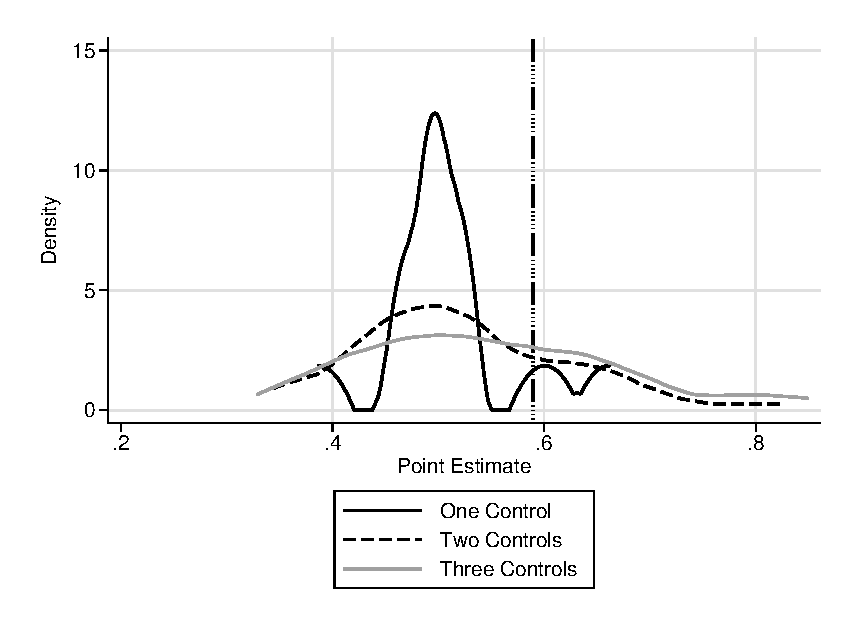
\includegraphics[width=\textwidth]{output/sencontrols_male_years_30y_itt_wctrl.eps}
\end{subfigure}%
\begin{subfigure}[h]{0.4\textwidth}
	\centering
	\caption{Employment, Males}
		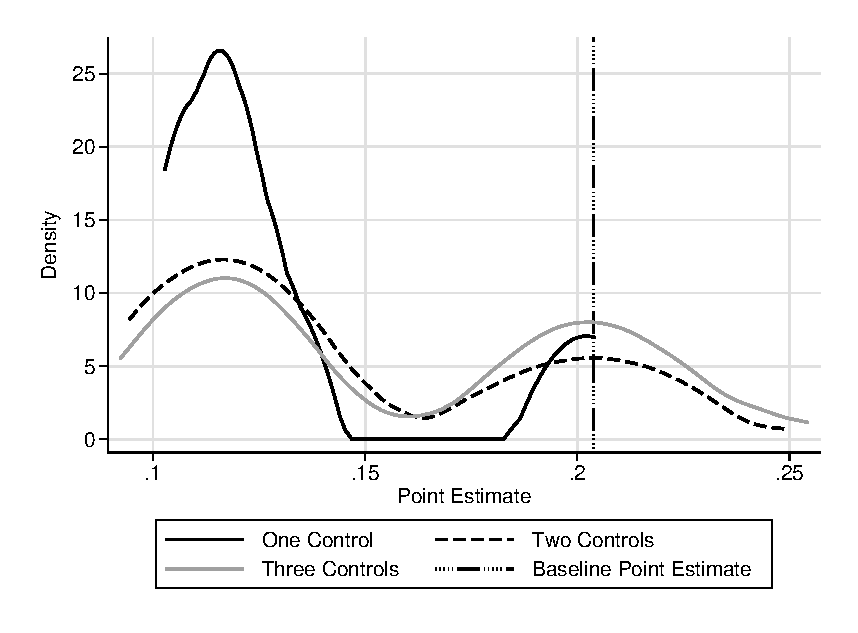
\includegraphics[width=\textwidth]{output/sencontrols_male_si30y_works_itt_wctrl.eps}
\end{subfigure}
\begin{subfigure}[h]{0.4\textwidth}
		\centering
		\caption{Years of Education, Females}
		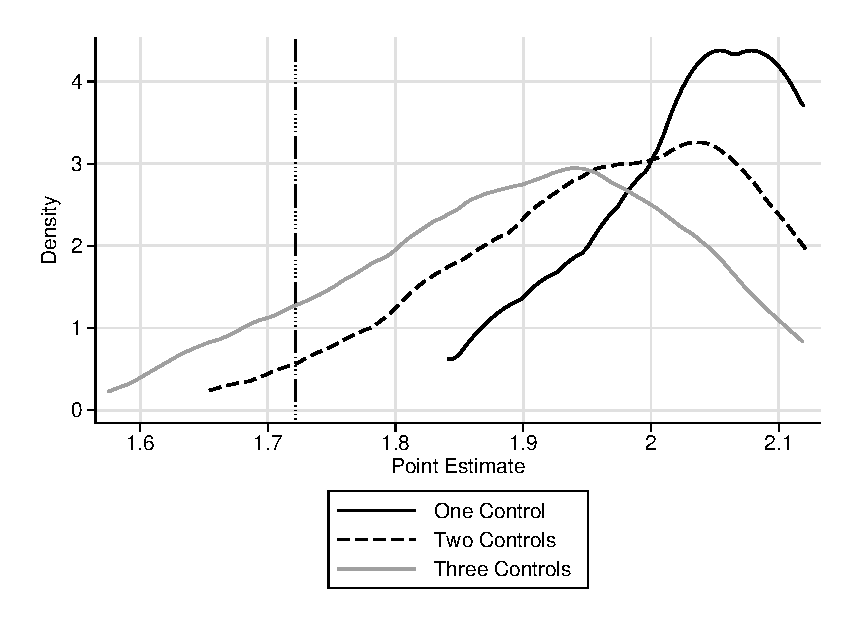
\includegraphics[width=\textwidth]{output/sencontrols_female_years_30y_itt_wctrl.eps}
\end{subfigure}%
\begin{subfigure}[h]{0.4\textwidth}
	\centering
	\caption{Employment, Females}
		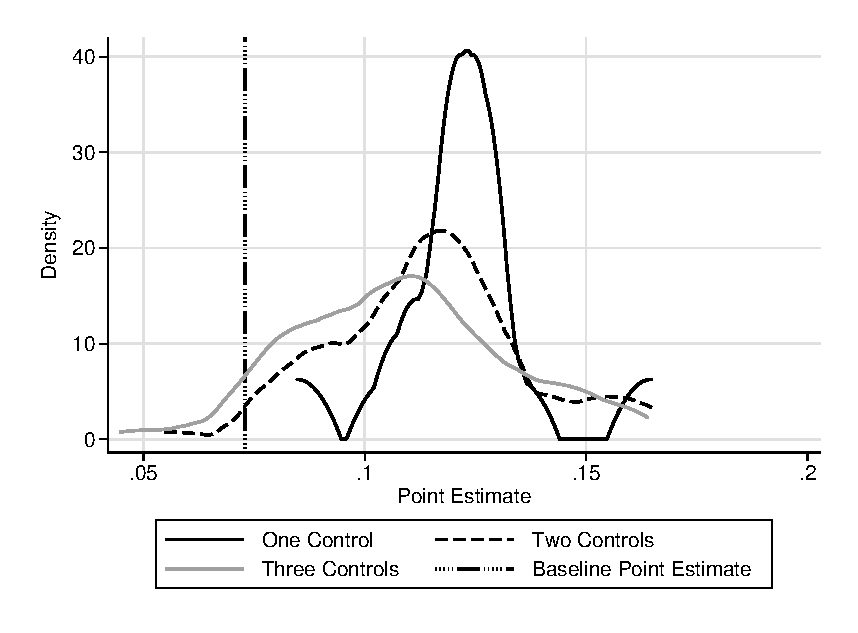
\includegraphics[width=\textwidth]{output/sencontrols_female_si30y_works_itt_wctrl.eps}
\end{subfigure}
\footnotesize \justify
Note: Panel (a) displays the distribution of the treatment effect estimate of the treatment compared to next best counterfactual for males years of education. The distribution is obtained by using all possible combinations of one, two, and three background variables listed in Table~\ref{tab:pselectvars}. In addition to these three variables, we account for a male indicator when computing estimates pooling males and females and a ABC/CARE indicator, to account for any difference in the programs---although we extensively document throughout the paper the similarities between them. The horizontal line marks the baseline estimate we use. The remaining panels present analogous distributions for the outcomes and genders indicated in the title.\\
\end{sidewaysfigure}

\begin{sidewaysfigure}[!htbp]
\centering
\caption{Sensitiviy to Choice of Control Set, Treatment vs. Stay at Home}
\begin{subfigure}[h]{0.4\textwidth}
		\centering
		\caption{Years of Education, Males}
		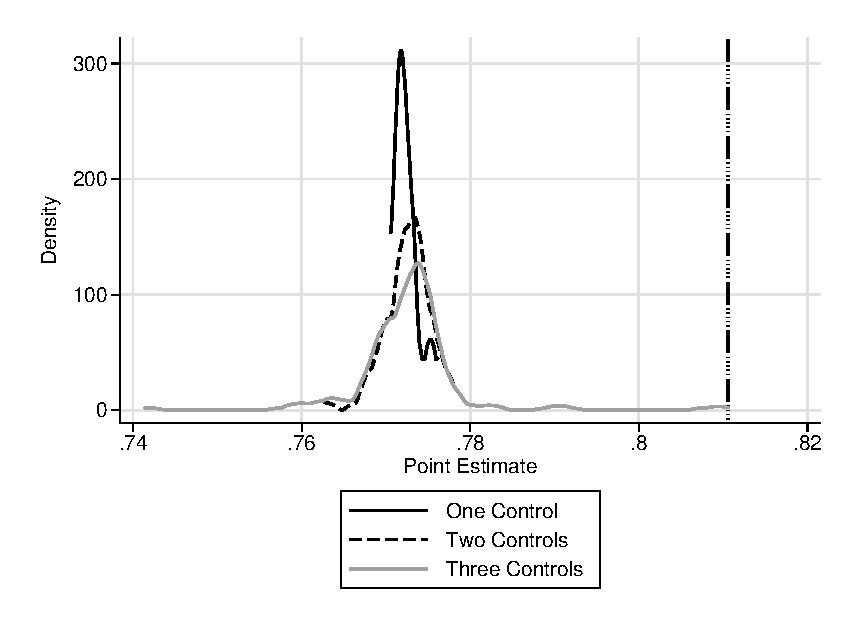
\includegraphics[width=\textwidth]{output/sencontrols_male_years_30y_epan_ipw_P0.eps}
\end{subfigure}%
\begin{subfigure}[h]{0.4\textwidth}
	\centering
	\caption{Employment, Males}
		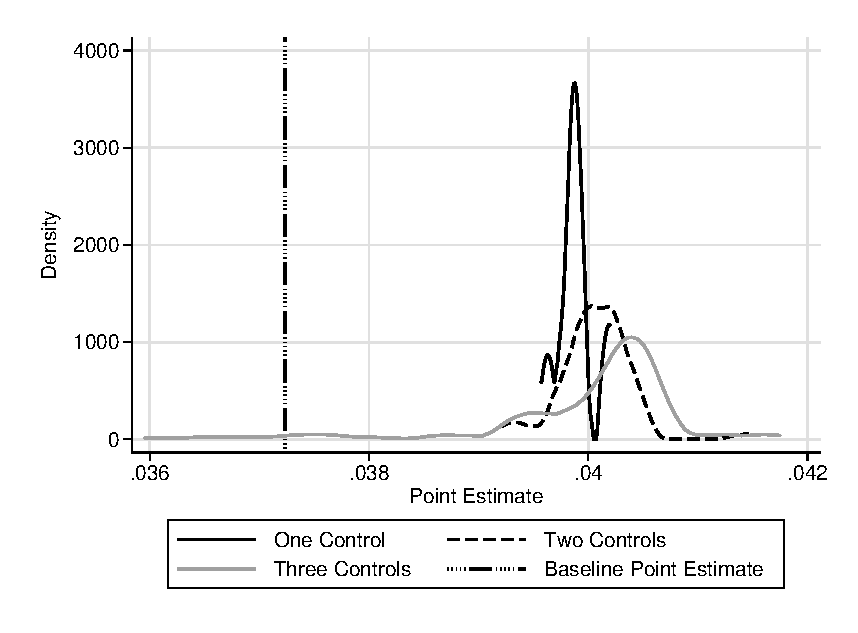
\includegraphics[width=\textwidth]{output/sencontrols_male_si30y_works_epan_ipw_P0.eps}
\end{subfigure}
\begin{subfigure}[h]{0.4\textwidth}
		\centering
		\caption{Years of Education, Females}
		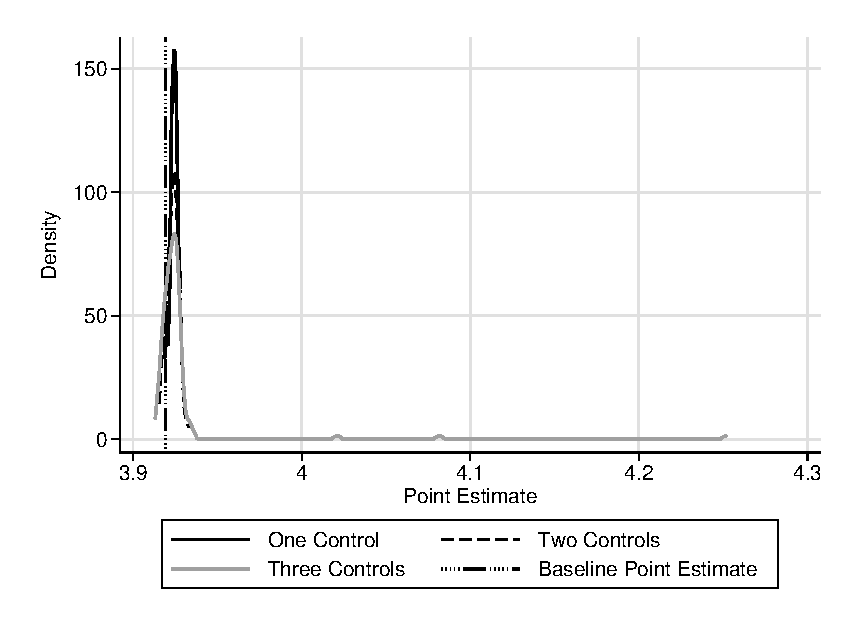
\includegraphics[width=\textwidth]{output/sencontrols_female_years_30y_epan_ipw_P0.eps}
\end{subfigure}%
\begin{subfigure}[h]{0.4\textwidth}
	\centering
	\caption{Employment, Females}
		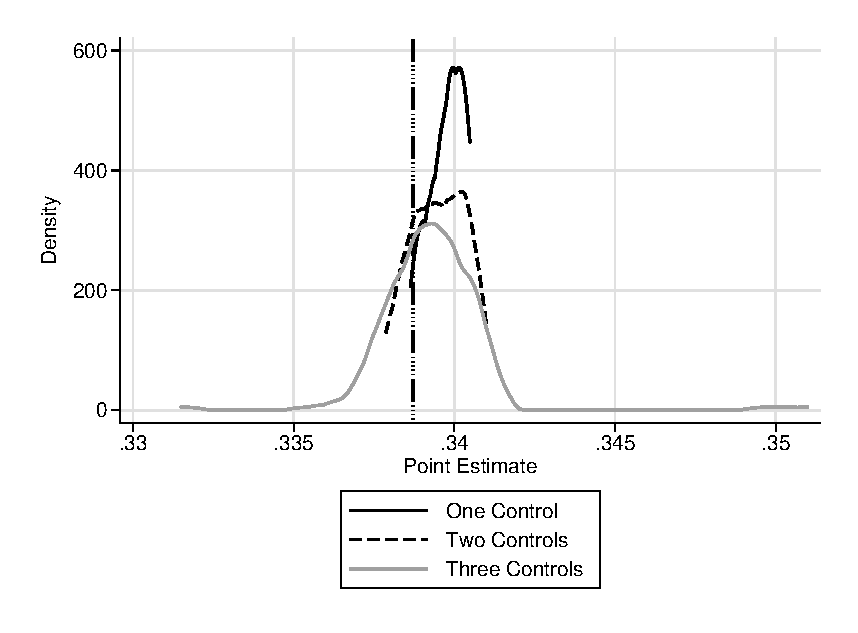
\includegraphics[width=\textwidth]{output/sencontrols_female_si30y_works_epan_ipw_P0.eps}
\end{subfigure}
\footnotesize \justify
Note: Panel (a) displays the distribution of the treatment effect estimate of the treatment compared to stay at home counterfactual for males years of education. The distribution is obtained by using all possible combinations of one, two, and three background variables listed in Table~\ref{tab:pselectvars}. In addition to these three variables, we account for a male indicator when computing estimates pooling males and females and a ABC/CARE indicator, to account for any difference in the programs---although we extensively document throughout the paper the similarities between them. We ``match'' and ``control'' using the same set of variables. The horizontal line marks the baseline estimate we use. The remaining panels present analogous distributions for the outcomes and genders indicated in the title.\\
\end{sidewaysfigure}

\begin{sidewaysfigure}[!htbp]
\centering
\caption{Sensitiviy to Choice of Control Set, Treatment vs. Alternative Preschool}\label{fig:senstap}
\begin{subfigure}[h]{0.4\textwidth}
		\centering
		\caption{Years of Education, Males}
		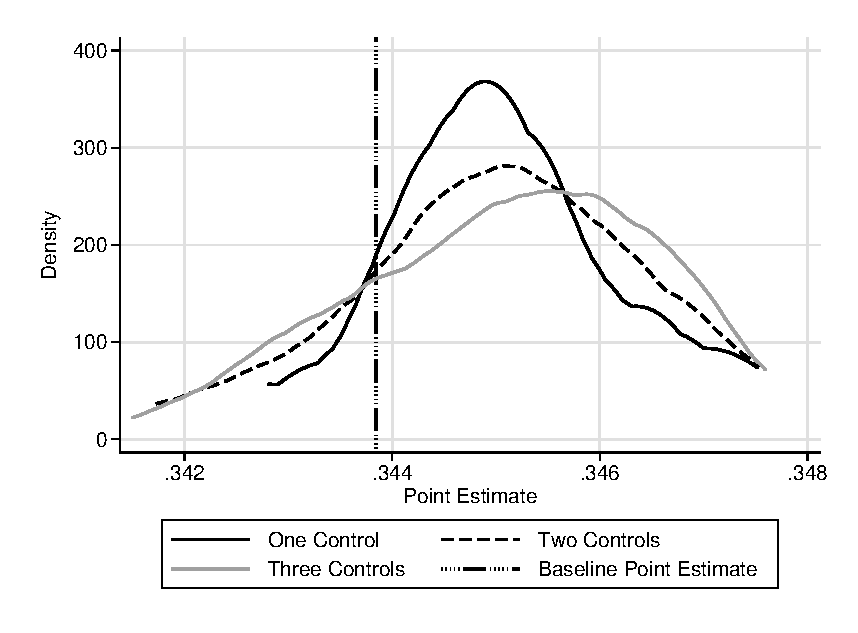
\includegraphics[width=\textwidth]{output/sencontrols_male_years_30y_epan_ipw_P1.eps}
\end{subfigure}%
\begin{subfigure}[h]{0.4\textwidth}
	\centering
	\caption{Employment, Males}
		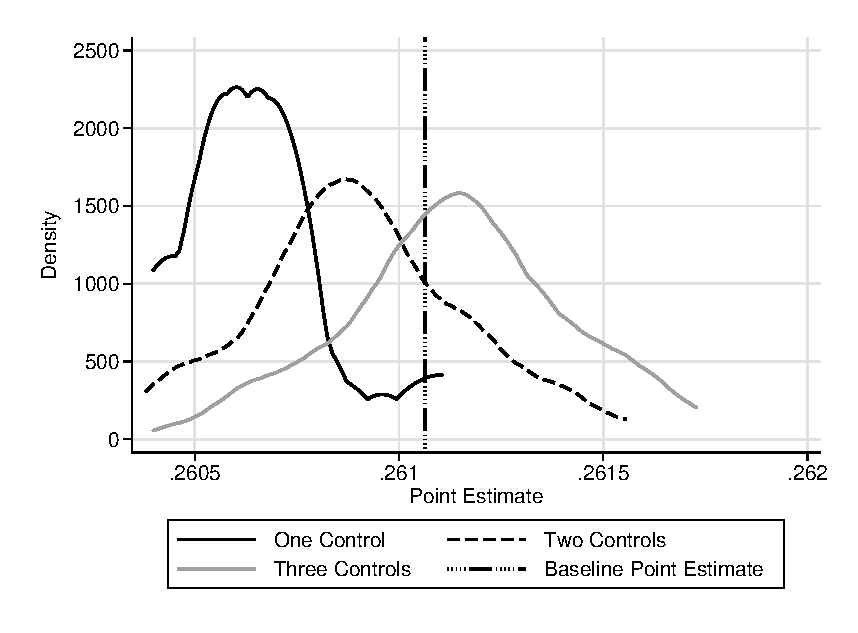
\includegraphics[width=\textwidth]{output/sencontrols_male_si30y_works_epan_ipw_P1.eps}
\end{subfigure}
\begin{subfigure}[h]{0.4\textwidth}
		\centering
		\caption{Years of Education, Females}
		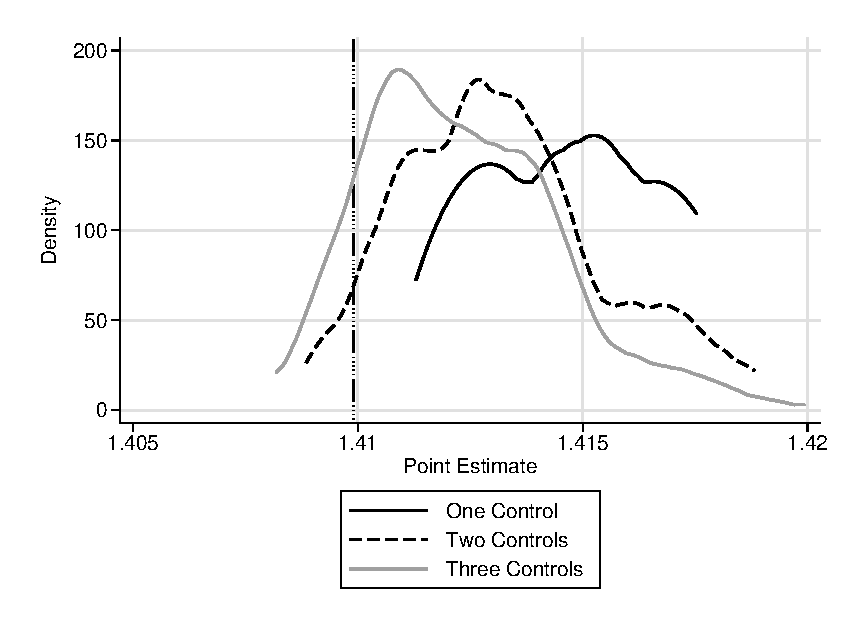
\includegraphics[width=\textwidth]{output/sencontrols_female_years_30y_epan_ipw_P1.eps}
\end{subfigure}%
\begin{subfigure}[h]{0.4\textwidth}
	\centering
	\caption{Employment, Females}
		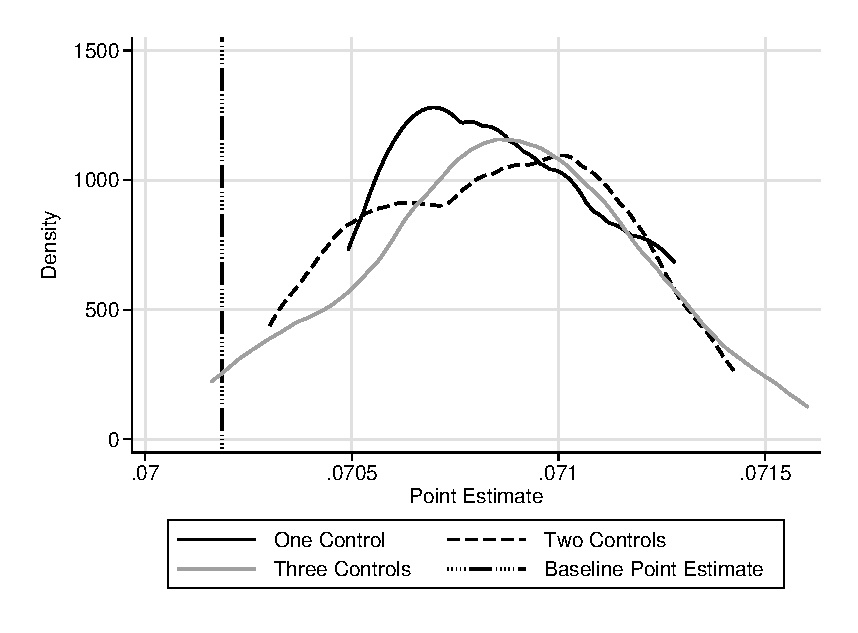
\includegraphics[width=\textwidth]{output/sencontrols_female_si30y_works_epan_ipw_P1.eps}
\end{subfigure}
\footnotesize \justify
Note: Panel (a) displays the distribution of the treatment effect estimate of the treatment compared to alternative preschool counterfactual for males years of education. The distribution is obtained by using all possible combinations of one, two, and three background variables listed in Table~\ref{tab:pselectvars}. In addition to these three variables, we account for a male indicator when computing estimates pooling males and females and a ABC/CARE indicator, to account for any difference in the programs---although we extensively document throughout the paper the similarities between them. We ``match'' and ``control'' using the same set of variables. The horizontal line marks the baseline estimate we use. The remaining panels present analogous distributions for the outcomes and genders indicated in the title.\\
\end{sidewaysfigure}



